\chapter{Discrétisation, algorithmes et exemples}
\label{chap:alorithme}
\minitoc

\[\]

Dans le précédent chapitre, la méthode a été élaborée dans un cadre continu, supposant un accès direct au domaine de calcul et à son champ de croix correspondant. Toutefois, dans la réalité, cette accessibilité directe n'est pas toujours envisageable. Ainsi, pour rendre cette méthode plus praticable, nous abordons dans ce chapitre une approche discrète, adaptant les différents algorithmes pour opérer sur des maillages triangulaires.

\'Etant donné un tel maillage représentant un domaine donné, le but de ce chapitre est de démontrer qu'à partir d'un champ de croix donné, il est possible de construire sur le maillage triangulaire un maillage quadrilatéral, et d'expliquer dans quelle mesure ce maillage représente fidèlement le domaine initial.

\section{Représentation discrète}

Soit $\Omega$ un domaine compact et connexe de $\mathbb{R}^2$ dont le bord $\partial\Omega$ est lisse par morceau. On désigne par $\bar{u}$ un champ de croix presque-$\mathcal{C}^1$ défini sur $\Omega$.

\subsection{Maillage triangulaire}

Considérons maintenant un maillage triangulaire $\Omega_h$ de $\Omega$. Par là, nous entendons que $\Omega_h$ est une surface polygonale compacte de $\mathbb{R}^2$ représentant une triangulation conforme de $\Omega$. Autrement dit, $\Omega_h$ formé par l'union de $N_t$ triangles fermés non vide: $\Omega_h=\cup_{k=1}^{N_t}T_k$ tel que tout intersection entre deux triangles est soit vide, soit un sommet, soit une arête. De plus, tous les sommets de $\Omega_h$ appartiennent à $\Omega$. Nous noterons $\mathcal{T}_h$ l'ensemble des triangles formant $\Omega_h$, l'indice $h$ faisant référence à la finesse du maillage, que l’on définit par le diamètre maximal des triangles constituant $\Omega_h$.
$$
h:=\max_{T\in\mathcal{T}_h} diam(T)
$$
Le diamètre d’un triangle est la distance maximale entre deux points du triangle. Nous notons de plus $\mathcal{A}_h$ et $\mathcal{S}_h$ les ensembles respectivement des sommets et des arêtes de $\Omega_h$. Pour tout $p\in\Omega_h$, Nous désignons par $T_p$ la partie du plan formé par l'ensemble des triangles de $\Omega_h$ contenant $p$: $T_p=\displaystyle\cup_{T\in\mathcal{T}_h\atop~p\in T~}T$.

\subsection{Champ de croix}

Nous cherchons maintenant à construire une représentation du champ de croix $\bar{u}$ sur le maillage triangulaire $\Omega_h$. Pour se faire, nous commençons par définir la notion d'angle signé entre deux croix.

\begin{definition}
Soient deux croix $\mathbf{c}_1,\mathbf{c}_2$ non nulles. L'angle signé entre $\mathbf{c}_1$ et $\mathbf{c}_2$ noté $\delta\theta(\mathbf{c}_1,\mathbf{c}_2$) est l'unique élément de l'ensemble:
$$
\{\delta\theta(\mathbf{c}_1,\mathbf{c}_2)\}:=\left\{\theta_{\mathbf{c}_2}-\theta_{\mathbf{c}_1}+k\frac{\pi}{2},~k\in\mathbb{Z}\right\}\cap\left]-\frac{\pi}{4}, \frac{\pi}{4}\right[.
$$
\end{definition}
Nous dirons que $\delta\theta(\mathbf{c}_1,\mathbf{c}_2$) n'est pas défini lorsque $|\theta_{\mathbf{c}_2}-\theta_{\mathbf{c}_1}|=\pi/4$. Cette fonction mesure la variation angulaire entre $\mathbf{c}_1$ et $\mathbf{c}_2$ de $\mathbf{c}_1$ vers $\mathbf{c}_2$. Autrement dit, on a:
$$
\theta_{\mathbf{c}_2}=\theta_{\mathbf{c}_1}+\delta\theta(\mathbf{c}_1,\mathbf{c}_2).
$$
Dans toute la suite, nous imposons les contraintes suivantes sur le maillage $\Omega_h$ :\\[-0.2cm]
\begin{itemize}
 \item pour chaque arête $a\in\mathcal{A}_h$ délimitée par les sommets $s_1$ et $s_2$, il est requis que $\bar{u}(s_1)\neq 0$ ou $\bar{u}(s_2)\neq 0$.\\[-0.2cm]
 \item De plus, dans le cas où $\bar{u}(s_1)\neq 0$ et $\bar{u}(s_2)\neq 0$, la quantité $\delta\theta(\bar{u}(s_1), \bar{u}(s_2))$ doit être définie.\\[-0.2cm]
\end{itemize}
Dans la pratique, il sera donc impératif d'affiner ou de modifier localement un maillage qui ne satisfait pas ces contraintes. La pertinence de ces contraintes prend tout son sens par la suite, avec l'approche de construction que nous proposons pour représenter $\bar{u}$ sur $\Omega_h$. Nous introduisons à présent le concept de triangle singulier avec la définition suivante :

\begin{definition}
\label{def:triangle_singulier}
 Un triangle $T$ de $\mathcal{T}_h$ et de sommets $s_1$, $s_2$ et $s_3$ est dit singulier si l'une des assertions suivantes est vérifiée:\\[-0.2cm]
 \begin{itemize}
  \item[i.)] il existe $i\in\llbracket 1, 3\rrbracket$ tel que $\bar{u}(s_i)=0$,\\[-0.2cm]
  \item[ii.)] $\sum_{i=1}^3\delta\theta(\bar{u}(s_i),\bar{u}(s_{i+1}))\neq 0$.
 \end{itemize}

\end{definition}

Avec ces concepts en main, nous décrivons à présent la représentation du champ de croix $\bar{u}$ sur $\Omega_h$ par un champ de croix $\bar{u}_h$. Ce dernier est défini pour tout $p\in\Omega_h$ par :\\
\begin{itemize}
\item[$\bullet$] si $p\in\mathcal{S}_h$, alors $\bar{u}_h(p)=\bar{u}(p)$,\\[-0.2cm]
\item[$\bullet$] si $p\in a$, où $a\in\mathcal{A}_h$ est une arête de sommets $s_1$ et $s_2$, alors on a:
$$
\left\{
\begin{array}{l}
\bar{u}_h(p)=\displaystyle\left\{\mathbf{R}\left(\theta_p+m\frac{\pi}{2}\right)(1,0)^t,~m\in\mathbb{Z}\right\},\\\\
\theta_p=\theta_{\bar{u}_h}(s_1)+\displaystyle\frac{\|\overrightarrow{s_1p}\|}{\|\overrightarrow{s_1s_2}\|}\delta\theta(\bar{u}_h(s_1),\bar{u}_h(s_2)).
\end{array}
\right.
$$
%\\[-0.2cm]
\item[$\bullet$] si $p\in T$ où $T\in\mathcal{T}_h$ est un triangle non-singulier, alors on pose :%\\[-0.3cm]
$$
\left\{
\begin{array}{l}
\theta_1 = \theta_{\bar{u}_h}(s_1)\\\\
\theta_2 = \theta_1 + \delta\theta(\bar{u}_h(s_1),\bar{u}_h(s_2))\\\\
\theta_3 = \theta_2 + \delta\theta(\bar{u}_h(s_2),\bar{u}_h(s_3))
\end{array}
\right.
$$
où $s_1$, $s_2$ et $s_3$ sont les sommets du triangle $T$. La croix $\bar{u}_h(p)$ est alors donnée par :
$$
\left\{
\begin{array}{l}
\bar{u}_h(p)=\displaystyle\left\{\mathbf{R}\left(\theta_p+m\frac{\pi}{2}\right)(1,0)^t,~m\in\mathbb{Z}\right\},\\\\
\theta_p=\displaystyle\sum_{i\in\llbracket1, 3\rrbracket}\lambda_i\theta_i,
\end{array}
\right.
$$
avec $(\lambda_i)_{i\in\llbracket 1, 3\rrbracket}$ les coordonnées barycentriques de $p$ dans le triangle $T$. Autrement dit, ils vérifient $p=\sum_{i=1}^3\lambda_i s_i$ et $\sum_{i=1}^3\lambda_i=1$.
\\[-0.2cm]
\item[$\bullet$] si $p\in T$ avec $T\in\mathcal{T}_h$ un triangle singulier  et $p$ barycentre de $T$ (c'est à dire $p=1/3(s_1+s_2+s_3)$ avec $s_1$, $s_2$ et $s_3$ les sommets de $T$) alors on pose $\bar{u}_h(p)=0$.\\[-0.2cm]
\item[$\bullet$] sinon $p$ appartient à un triangle singulier $T$ tel qu'il existe $q\in T$ avec $\bar{u}_h(q)=0$. La croix $\bar{u}_h(p)$ est alors donnée par:
$$
\left\{
\begin{array}{l}
\bar{u}_h(p)=\bar{u}_h(\widetilde{p}),\\\\
\{\widetilde{p}\}=[qp)\cap\partial T_q.
\end{array}
\right.
$$
Noter que l'ensemble $[qp)\cap\partial T_q$ est bien réduit à un singleton puisque $T_q$ est une réunion de simplexes donc convexe.
\end{itemize}

\begin{remark}
La variation angulaire du champ de croix le long des arêtes du maillage constitue le fondement de la représentation mentionnée précédemment. Il est donc essentiel de pouvoir définir les croix en chaque point le long de chaque arête, d'où la pertinence des contraintes imposées au maillage précédemment évoquées.
\end{remark}


\begin{comment}
\subsection*{Maillage triangulaire et représentation des  champs de croix}

Considérons maintenant une triangulation h de la surface Ω. Par là, nous entendons que h est une surface polyédrique orientable compacte de dimension deux, de classe C0, et en notant Th l'ensemble des triangles fermés non vides tels que $∪T \in Th T = Ω$, nous supposons que tous les sommets appartiennent à Ω, et que toute intersection entre deux triangles est soit vide, soit un sommet, soit un côté. Soit $h_T = diam(T) et h = max{h_T : T \in Th}$

Considérons $\Omega$ comme un domaine borné et fermé dans $\mathbb{R}^2$. Pour le représenter, nous utilisons un maillage triangulaire noté $\Omega_h=(V, E, F)$, où $h$ est la taille des éléments du maillage. Ici, $V$ désigne l'ensemble des sommets de $\Omega_h$, $E$ représente l'ensemble des arêtes, et $F$ correspond à l'ensemble des triangles qui composent $\Omega_h$. Si $\bar{u}$ est un champ de croix défini sur $\Omega$, on se donne un ensemble de valeurs de $\bar{u}$ défini sur les sommets de $\Omega_h$. Une représentation $\bar{u}_h$ de $\bar{u}$ est alors construite pour tout $p\in\Omega_h$ de la manière suivante:

\begin{equation}
    \bar{u}_h(p) =
\left\{ 
    \begin{array}{lc}
        \displaystyle\left\{\mathbf{R}\left(\frac{m\pi}{2}\right)
        \begin{pmatrix} 
          cos(\arg{g(p)}/4)\\\\
          sin(\arg{g(p)}/4)
        \end{pmatrix},
        ~ m\in \mathbb{Z}\right\} &\text{ si }g(p)\neq (0, 0)\\\\
        0& \text{sinon}
    \end{array} 
\right.
\label{eqn:def_u_h}
\end{equation}
où $g$ est définie pour tout $p\in\Omega_h$ par:
\begin{equation}
    g(p)=\sum_{i=1}^3\lambda_i
    \begin{pmatrix} 
      cos(4\theta_{\bar{u}_h}(s_i))\\\\
      sin(4\theta_{\bar{u}_h}(s_i))
    \end{pmatrix},
\end{equation}
avec $(s_i)_{i\in\llbracket 1, 3\rrbracket}$ les sommets d'un triangle de $\Omega_h$ contenant $p$ et $(\lambda_i)_{i\in\llbracket 1, 3\rrbracket}$ les coordonnées barycentriques de $p$ dans ce triangle. Remarquons que le champ de croix $\bar{u}_h$ ainsi défini est presque-$\mathcal{C}^1$ sur chaque triangle puisque $g$ est linéaire sur chaque triangle.
\end{comment}

\subsection{Points singuliers, indice et ligne de champs}

L'ensemble $\mathcal{S}_{\bar{u}_h}$, défini comme l'ensemble des points singuliers de $\bar{u}_h$, est constitué des points $p \in \Omega_h$ tels que $\bar{u}_h(p) = 0$.
\begin{lemma}
    Les points singuliers de $\bar{u}_h$ sont isolés.
\end{lemma}
\begin{proof}
    Soit $q$ un point singulier de $\bar{u}_h$. Le point $q$ est isolé puisque par construction, on a $T_q\cap\mathcal{S}_{\bar{u}_h}=\{q\}$. En effet, pour tout $p\in T_q\backslash\{q\}$ on a $\bar{u}_h(p)=\bar{u}_h(\widetilde{p})$ où $\widetilde{p}$ est le point d'intersection entre la demi-droite $[qp)$ et le bord $\partial T_q$ de $F_q$. Il existe donc une arête $a\in\mathcal{A}_h$ vérifiant $a\subset\partial T_q$ et contenant le point $\widetilde{p}$. Par ailleurs pour tout $r\in a$, on a $\bar{u}_h(r)\neq 0$ par construction puisque $\bar{u}_h(s_1)\neq 0$ et $\bar{u}_h(s_2)\neq 0$ (avec $s_1$ et $s_2$ les sommets de $a$). Il vient alors que $\bar{u}_h(\widetilde{p})\neq 0$ et par conséquent $p\notin \mathcal{S}_{\bar{u}_h}$. Autrement dit, $T_q\cap\mathcal{S}_{\bar{u}_h}=\{q\}$.
\end{proof}

Examinons à présent l'indice des points singuliers de $\bar{u}_h$. Soit $p$ un point singulier de $\bar{u}_h$ avec $p\in\Omega_h\backslash\partial\Omega_h$. L'indice de $p$ est donné par:
$$
id_{\bar{u}_h}(p)=\frac{1}{2\pi}\int_0^1 d\theta^\gamma_{\bar{u}_h}=\frac{1}{2\pi}\sum_{\gamma_T\in\{\gamma\cap T,~T\in\mathcal{T}_h\}}\int_0^1 d\theta^{\gamma_T}_{\bar{u}_h}.
$$
où $\gamma$ est un chemin fermé paramétré sur $[0, 1]$ englobant $p$ et ne contenant aucun autre point singulier de $\bar{u}_h$. En pratique, nous calculerons l'indice d'un point $p$ en utilisant une paramétrisation $\gamma$ du bord $\partial F_p$ de $F_p$. De ce fait, l'indice du point $p$ s'écrit:
\begin{equation}
    \label{eqn:ind_int}
    id_{\bar{u}_h}(p)=\displaystyle\frac{1}{2\pi}\displaystyle\sum_{i=1}^{n_s}\left(\theta^\gamma_{\bar{u}_h}(s_{i+1})-\theta^\gamma_{\bar{u}_h}(s_i)\right)=\displaystyle\frac{1}{2\pi}\sum_{i=1}^{n_s}\delta\theta(\bar{u}_h(s_i),\bar{u}_h(s_{i+1})),
\end{equation}
où $(s_i)_{i\in\llbracket 1, n_s\rrbracket}=\mathcal{S}_h\cap\partial T_p$ désigne l'ensemble des sommets des triangles formant $T_p$, privés du point $p$, et numérotés dans le sens positif avec $s_{n_s+1}:=s_1$.
Si $p\in\partial\Omega_h$ alors l'indice de $p$ est donné par:
\begin{equation}
    \label{eqn:ind_bord}
    id_{\bar{u}_h}(p)=\displaystyle\frac{1}{2\pi}\left[\pi-\widehat{p}+\displaystyle\sum_{i=1}^{n_s}\left(\theta^\gamma_{\bar{u}_h}(s_{i+1})-\theta^\gamma_{\bar{u}_h}(s_i)\right)\right]=\displaystyle\frac{1}{2\pi}\left[\pi-\widehat{p}+\displaystyle\sum_{i=1}^{n_s}\left(\theta^\gamma_{\bar{u}_h}(s_{i+1})-\theta^\gamma_{\bar{u}_h}(s_i)\right)\right],
\end{equation}
où $\gamma$ dans ce cas est la paramétrisation de $\partial T_p\backslash\partial\Omega_h$ (c'est à dire la partie de $\partial T_p$ se trouvant à l'intérieur de $\Omega_h$) et $(s_i)_{i\in\llbracket 1, n_s\rrbracket}$ l'ensemble des sommets de $\Omega_h$ appartenant à $\partial T_p\backslash\partial\Omega_h$.

\begin{proposition}
    Pour tout $p\in\Omega_h\backslash\partial\Omega_h$, on a $4id_{\bar{u}_h}(p)\in\rrbracket -n_a/4, n_a/4\llbracket$ où $n_a$ est le nombre d'arête inclut dans $\partial T_p$.
\end{proposition}

\begin{proof}
Soit $p\in\Omega_h$. On sait que:
$$
id_{\bar{u}_h}(p)=\displaystyle\frac{1}{2\pi}\sum_{i=1}^{n_s}\delta\theta(\bar{u}_h(s_i),\bar{u}_h(s_{i+1})).
$$
Or pour tout $i\in\llbracket 1, n_s\rrbracket$, on a $\delta\theta(\bar{u}_h(s_i),\bar{u}_h(s_{i+1}))\in]-\frac{\pi}{4}, \frac{\pi}{4}[$. Autrement dit,
$$
\displaystyle\frac{1}{2\pi}\sum_{i=1}^{n_s}\delta\theta(\bar{u}_h(s_i),\bar{u}_h(s_{i+1}))\in\left]-\frac{n_s}{8}, \frac{n_s}{8}\right[.
$$
Or on sait que $4id_{\bar{u}_h}\in\mathbb{Z}$ et $n_s=n_a$. Par conséquent,
$$
4id_{\bar{u}_h}(p)\in\left\rrbracket-\frac{n_a}{4}, \frac{n_a}{4}\right\llbracket.
$$
\end{proof}
Un corollaire direct de la proposition précédente est que si un point singulier est localiser à l'intérieur d'un triangle alors les seuls indices possible pour ce point sont $-1/4, 0$ et $1/4$.

Nous abordons à présent la représentation des lignes de champs de $\bar{u}_h$ dans $\Omega_h$. Rappelons que étant donné un point $p_0\in\Omega_h$ et un vecteur $\overrightarrow{u_0}\in\mathbb{R}^2$, la ligne de champ $SL_{\bar{u}_h}(p_0, \overrightarrow{u_0})$ d'origine $p_0$ est la courbe $S$ telle que :

\begin{enumerate}
\item il existe $\pi_{\bar{u}_h}^S:\Omega_h\longrightarrow\mathbb{R}^2$ une application telle que $\pi_{\bar{u}_h}^S(p_0)=\overrightarrow{u_0}$ et pour tout $p\in Im S$ il existe un voisinnage $V_p$ de $p$ tel que:
\begin{equation}
\pi_{\bar{u}_h}^S\in\mathcal{C}^1(V_p) \mbox{ et }  \forall q\in V_p, \pi_{\bar{u}_h}^S(q)\in \bar{u}_h(q),
\end{equation}
\item $S$ est une solution maximale dans $\Omega$ de l'équation différentielle
\begin{equation}
\frac{dS(t)}{dt}=\pi_{\bar{u}_h}^S(S(t)),t\in \mathbb{R} \text{ et }  S(0)=p_0.
\end{equation}
\end{enumerate}
Pour représenter cette ligne de champ, nous procédons à la construction d'une approximation $SL^h_{\bar{u}_h}(p_0, \overrightarrow{u_0})$ de $SL_{\bar{u}_h}(p_0, \overrightarrow{u_0})$ sur $\Omega_h$ sous la forme d'une succession de segments. Le premier segment est représenté par $[p_0p_1]$ où $p_1$ est le point d'intersection entre $\partial T_{p_0}$ et la demi-droite d'origine $p_0$ et de vecteur directeur $\overrightarrow{u_0}$. Ensuite, pour tout $i\geq 1$, on construit le segment  $[p_ip_{i+1}]$ en cherchant le point $p_{i+1}$ comme le point d'intersection entre $\partial T_{p_i}$ et la demi-droite d'origine $p_i$ et dirigée par le vecteur
$$
\overrightarrow{u_i}=\mathbf{P}(\bar{u}_h(p_i), \overrightarrow{p_{i-1}p_i})+\mathbf{P}(\bar{u}_h(p'_{i+1}), \overrightarrow{p_{i-1}p_i}).
$$
Dans cette formule, $p'_{i+1}$ est le point d'intersection entre $\partial T_{p_i}$ et la demi-droite d'origine $p_i$ et dirigé par le vecteur $\mathbf{P}(\bar{u}_h(p_i), \overrightarrow{p_{i-1}p_i})$ et pour tout $(\mathbf{c},d)\in\mathbf{C}\backslash\{0\}\times\mathbb{R}^2$, $\mathbf{P}(\mathbf{c}, d)$ désigne le vecteur $\mathbf{c}$ qui s'aligne le mieux avec la direction $d$. Autrement dit, il s'agit de l'unique élément de l'ensemble
$$
\{\mathbf{P}(\mathbf{c}, d)\}=\underset{c_k\in\mathbf{c},~k\in\llbracket1, 4\rrbracket}{\mathrm{argmin}}|c_k.d.\|d\|^{-1}-1|.
$$
Une illustration de ce processus est donné sur la figure \ref{fig:draw_streams_1}.  Une alternative plus pratique et plus rapide pour la construction des segments $[p_ip_{i+1}]$ pour $i\geq 1$ consiste à exploiter la\\
Soit $S\cap T$

\begin{figure}[!h]
     \centering
     \begin{subfigure}[b]{0.7\textwidth}
         \centering
         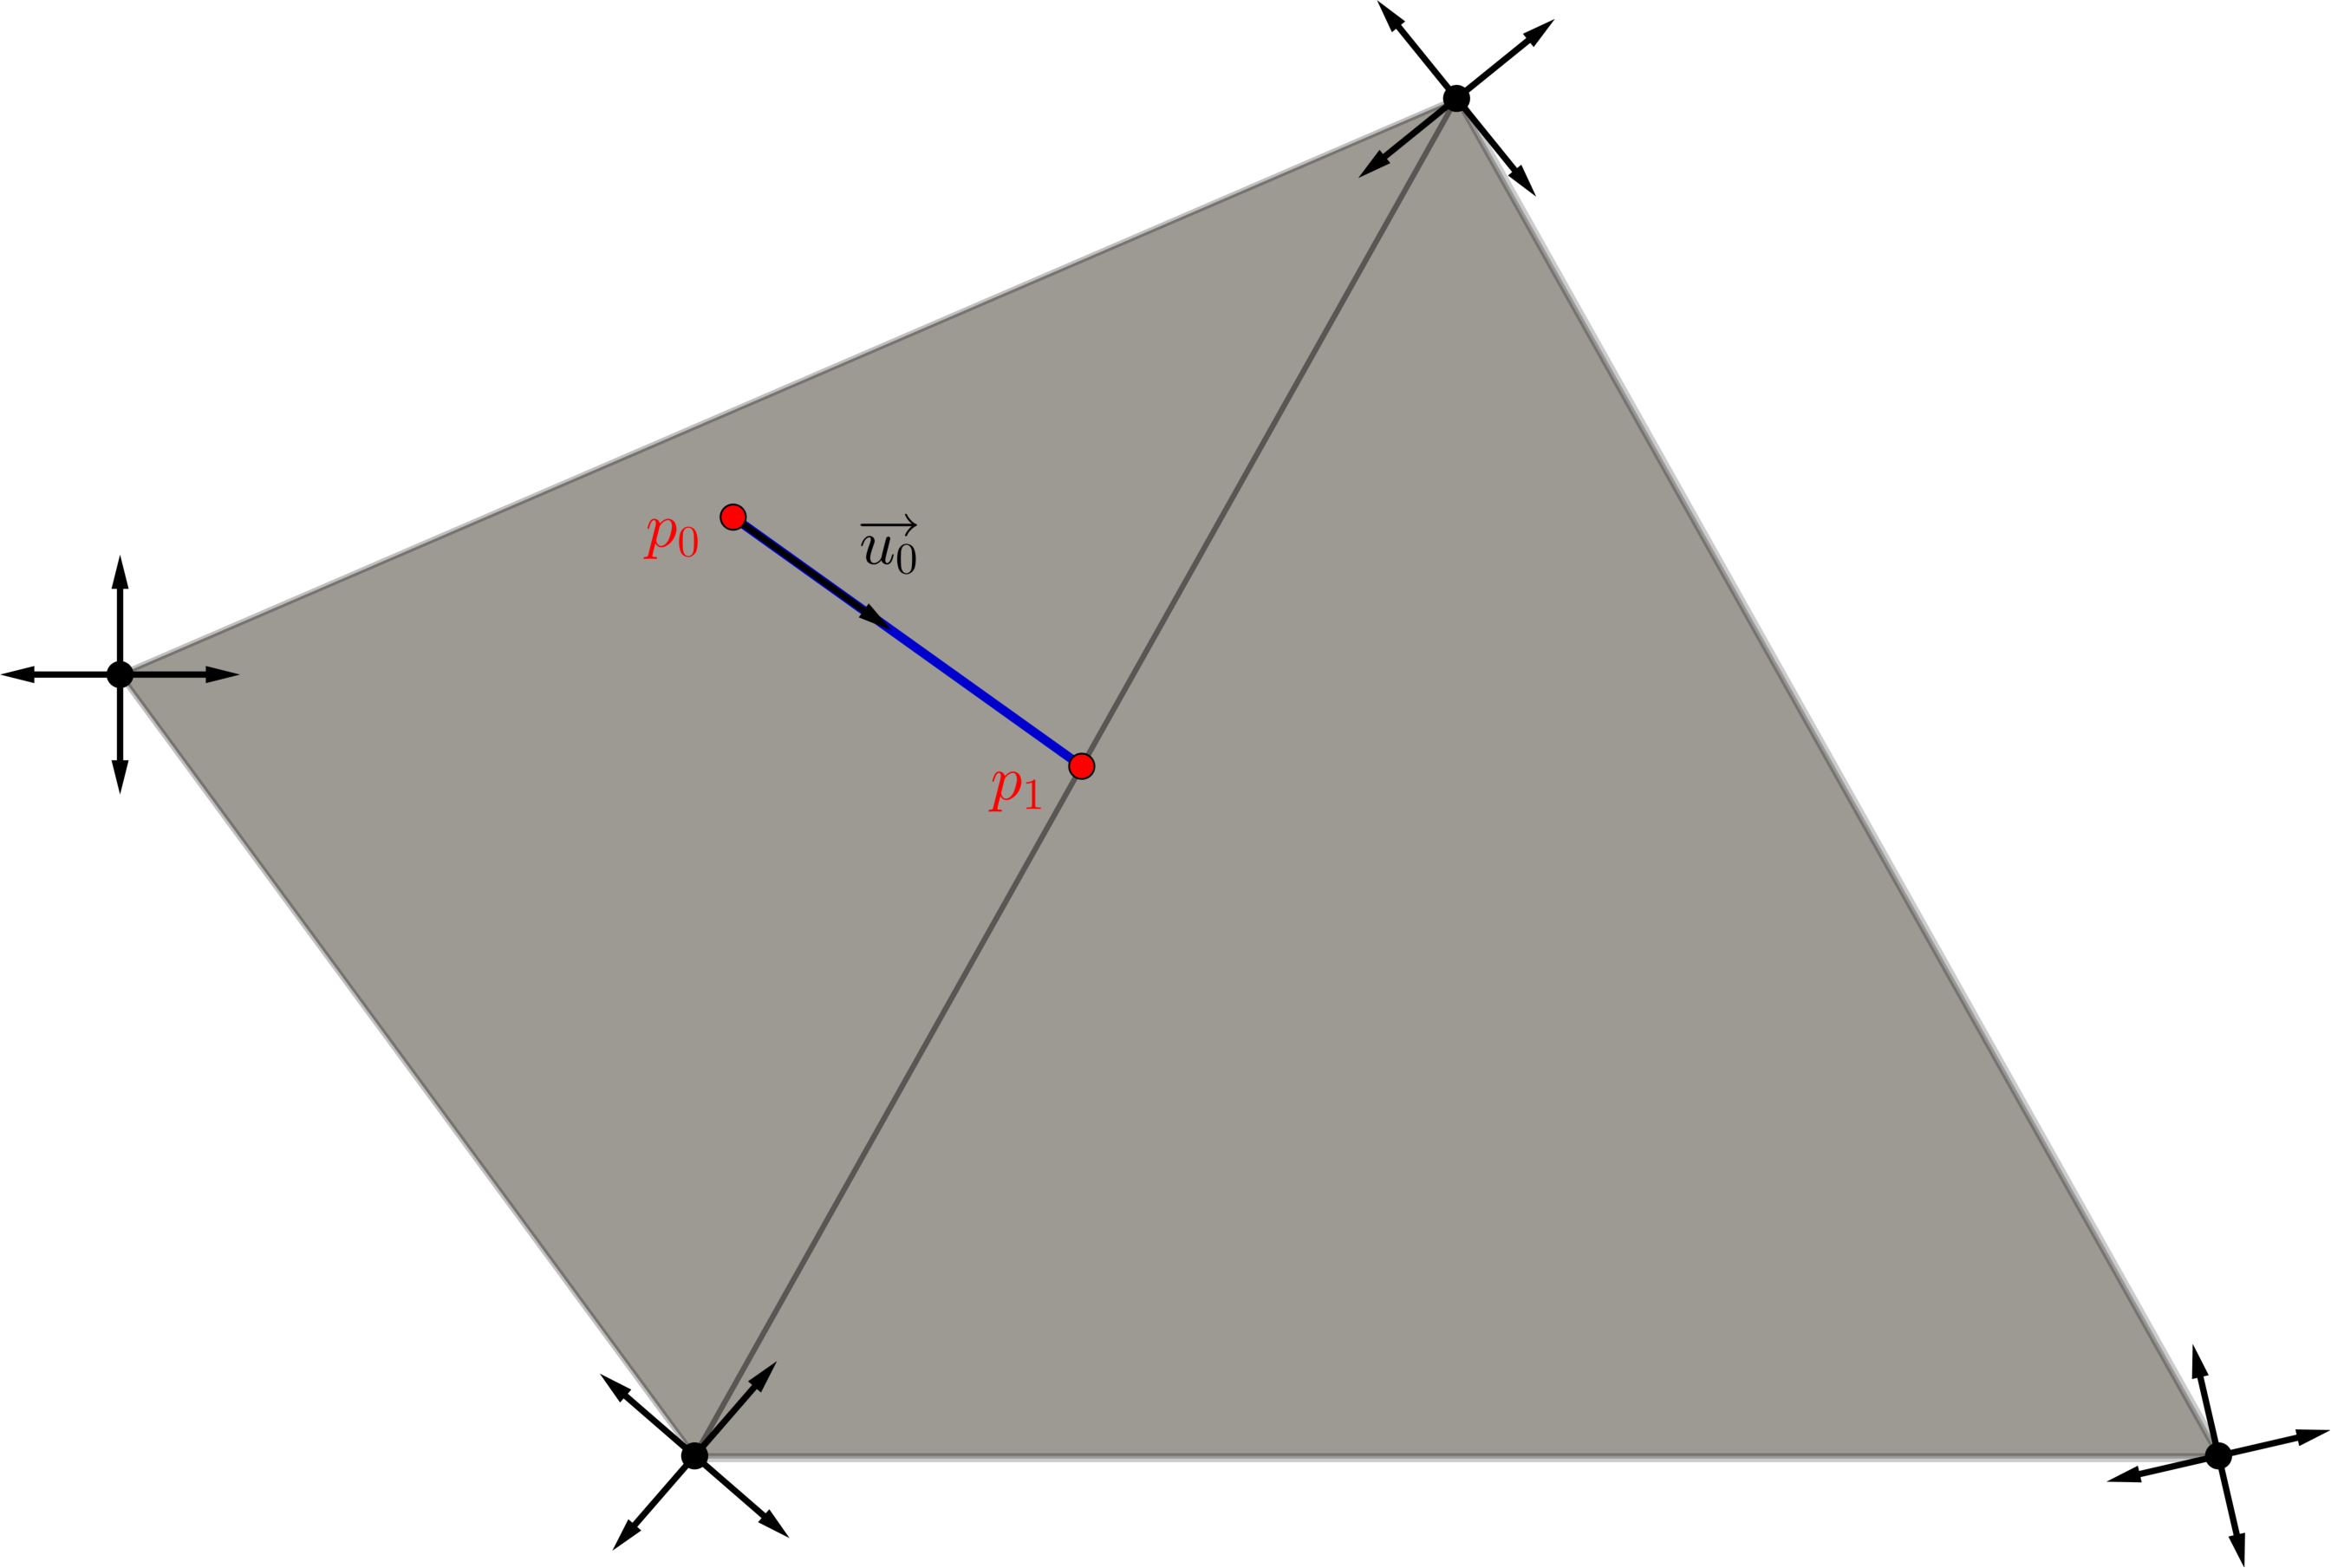
\includegraphics[width=\textwidth]{images/draw_streams_11.pdf}
         \caption{$y=x$}
         \label{fig:y equals x}
     \end{subfigure}
     \begin{subfigure}[b]{0.7\textwidth}
         \centering
         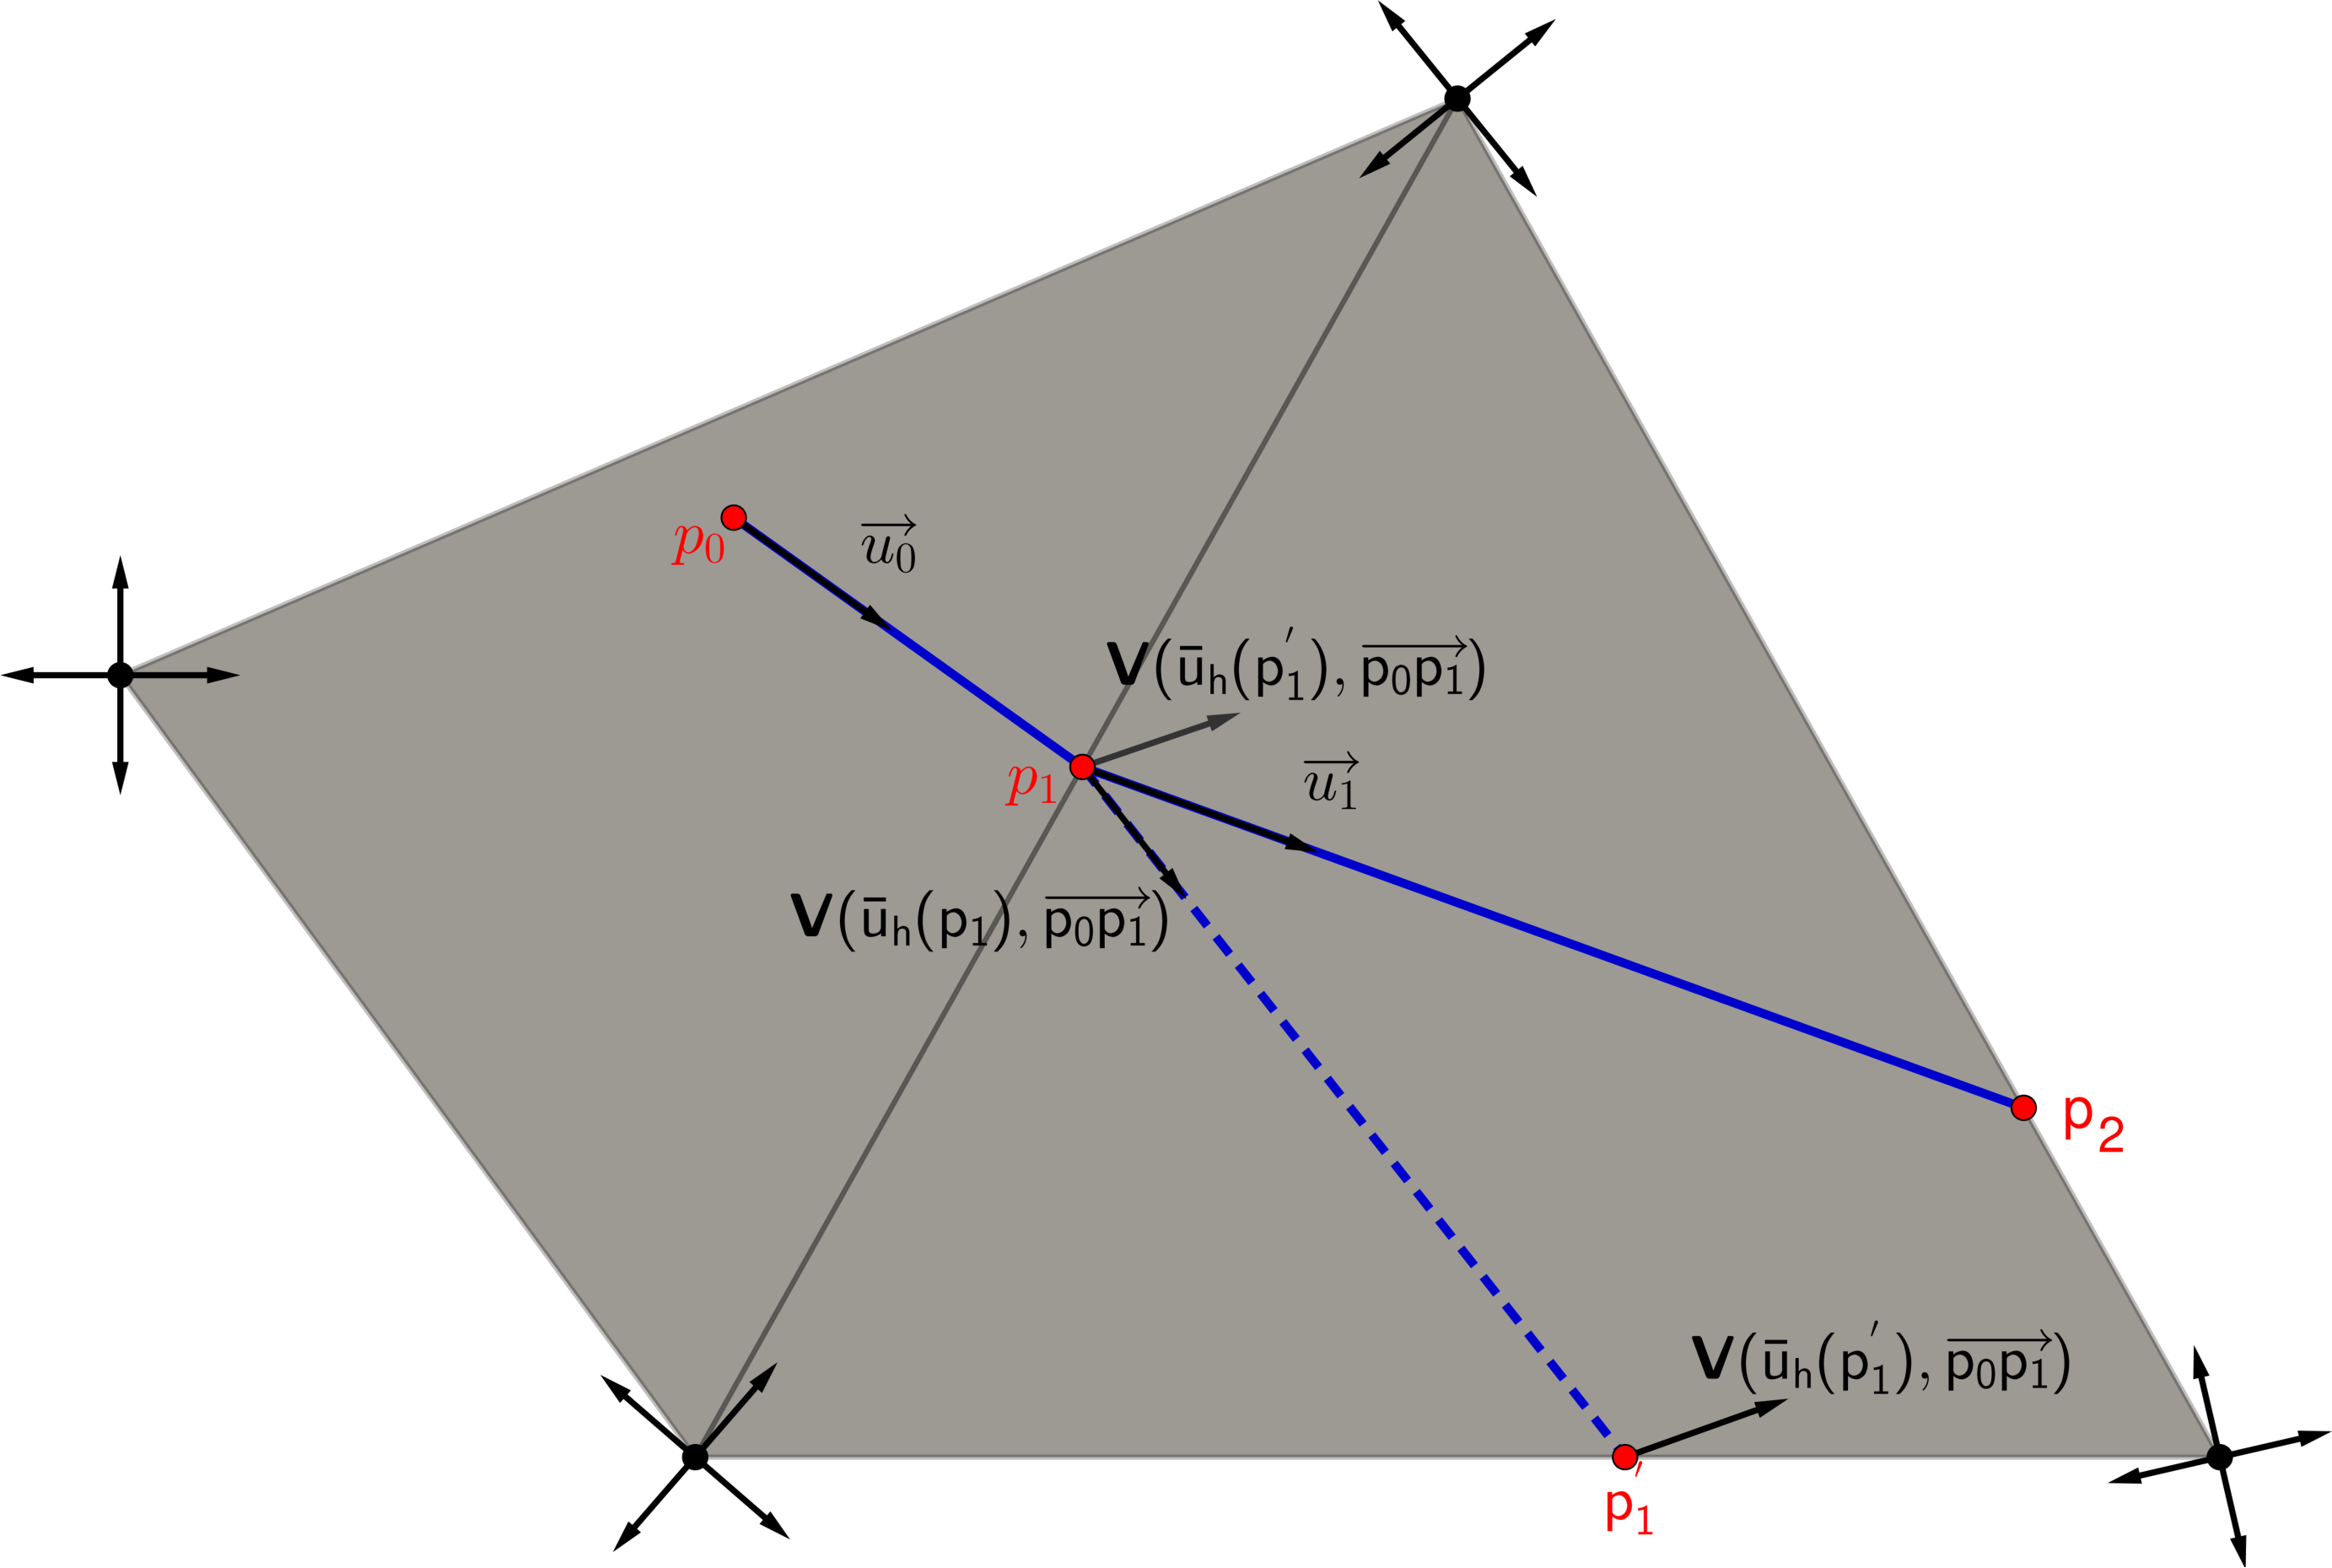
\includegraphics[width=\textwidth]{images/draw_streams_12.pdf}
         \caption{$y=3\sin x$}
         \label{fig:three sin x}
     \end{subfigure}
        \caption{Three simple graphs}
        \label{fig:draw_streams_1}
\end{figure}

\begin{figure}[!h]
     \centering
     \begin{subfigure}[b]{0.7\textwidth}
         \centering
         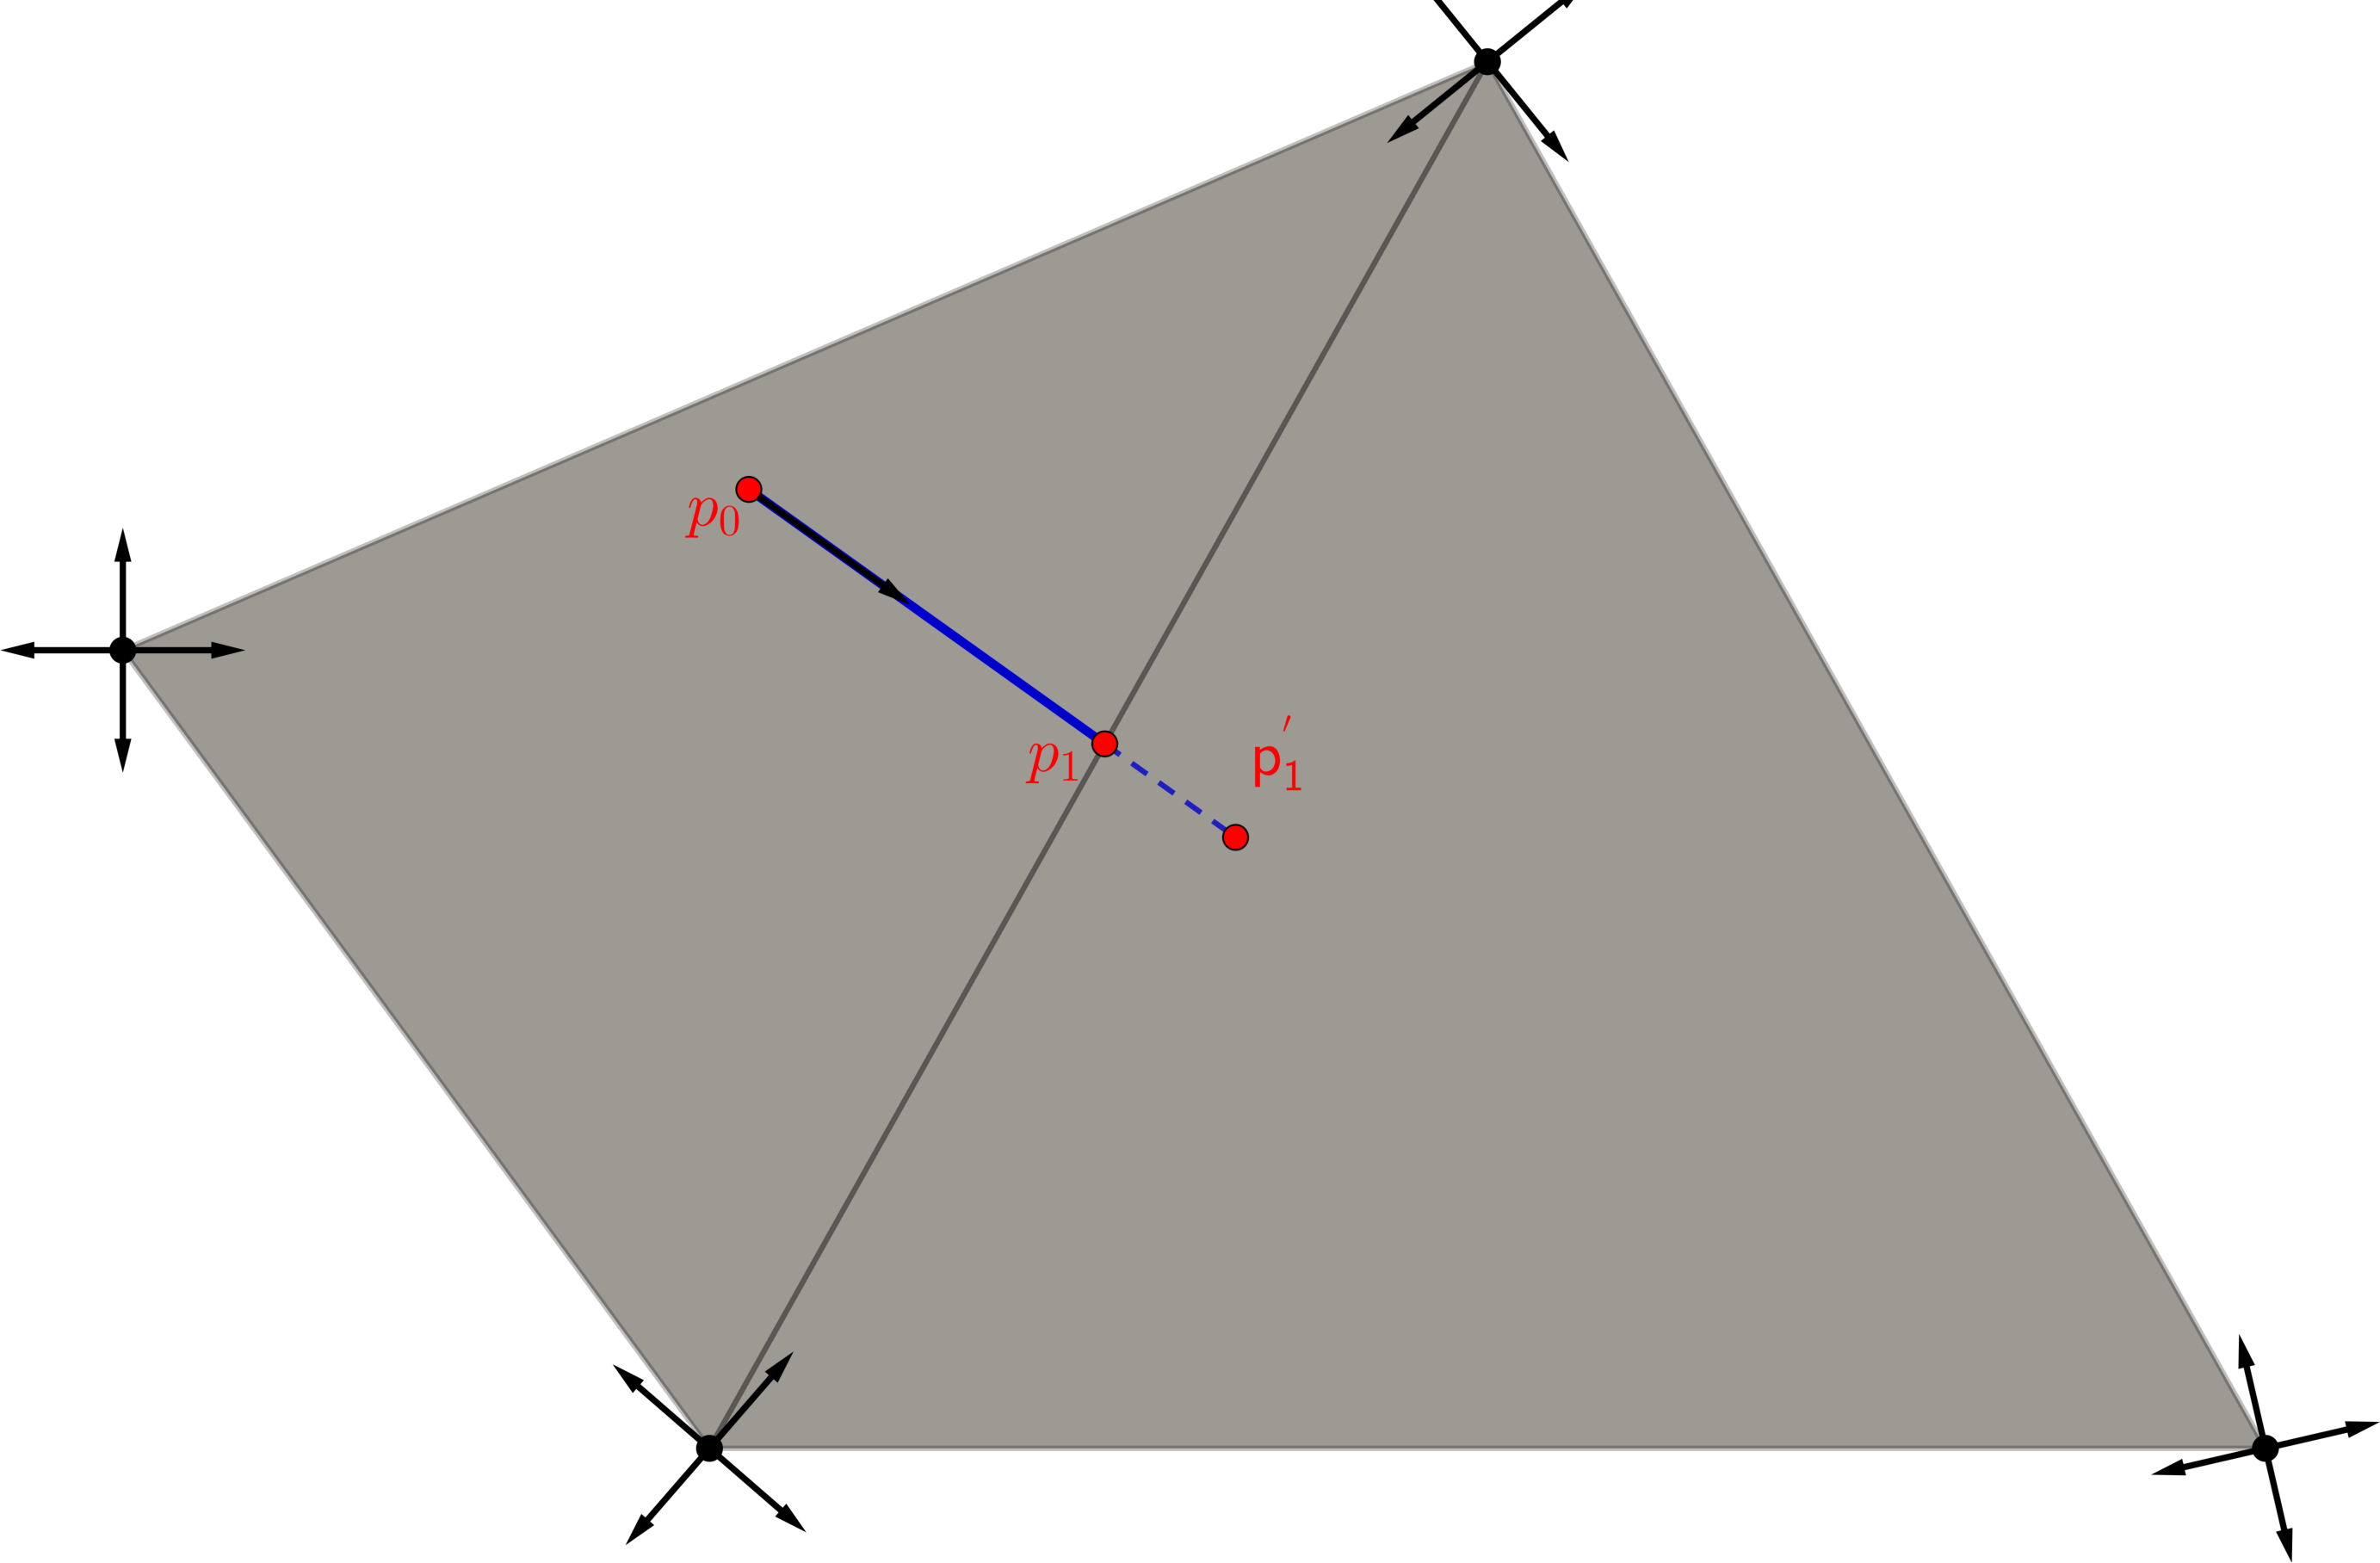
\includegraphics[width=\textwidth]{images/draw_streams_21.pdf}
         \caption{$y=x$}
         \label{fig:y equals x}
     \end{subfigure}
     \begin{subfigure}[b]{0.7\textwidth}
         \centering
         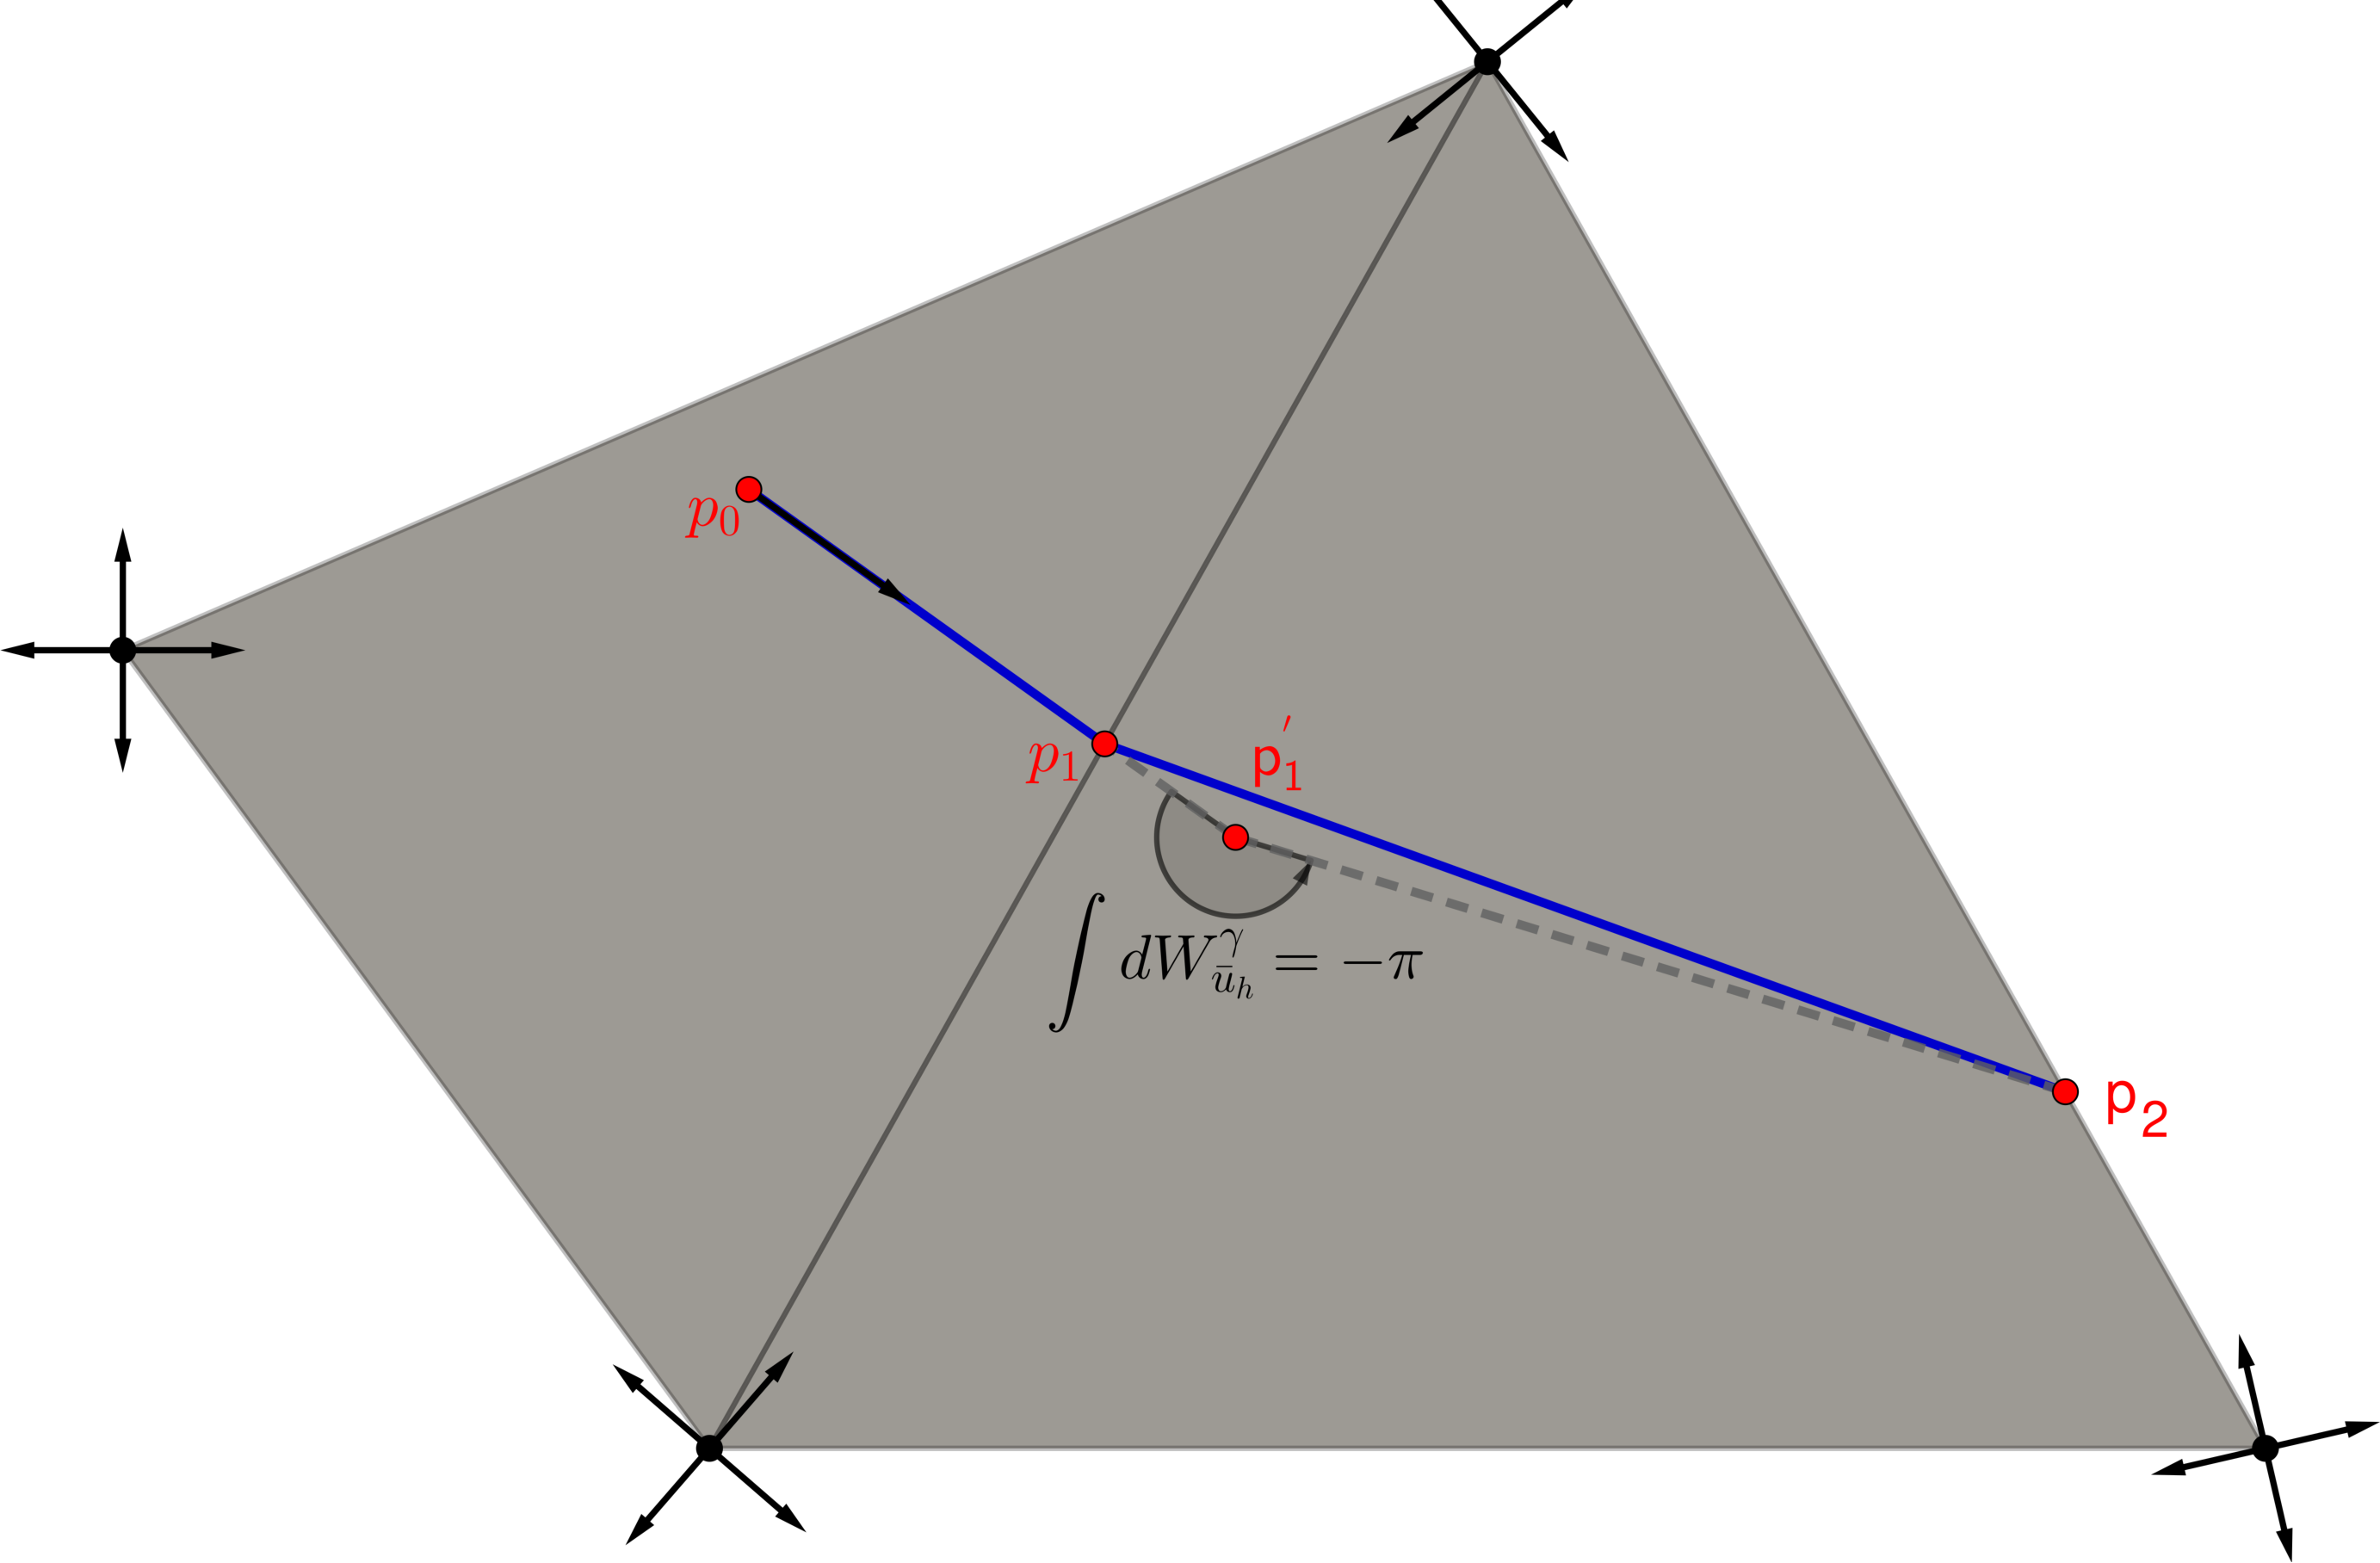
\includegraphics[width=\textwidth]{images/draw_streams_22.pdf}
         \caption{$y=3\sin x$}
         \label{fig:three sin x}
     \end{subfigure}
        \caption{Three simple graphs}
        \label{fig:draw_streams_1}
\end{figure}


\subsection{Lien entre $\bar{u}$ et $\bar{u}_h$}

\begin{lemma}
    $\mathcal{S}_{\bar{u}}=\mathcal{S}_{\bar{u}_h}$
\end{lemma}

Lorsque h tend vers 0, uh tend vers u\\z


Illustrer les singularité se démultipliant  en coloriant juste les triangles et en disant qu'on a pas besoin de la localisation spécifique.\\

\begin{figure}[!h]
  \centering
  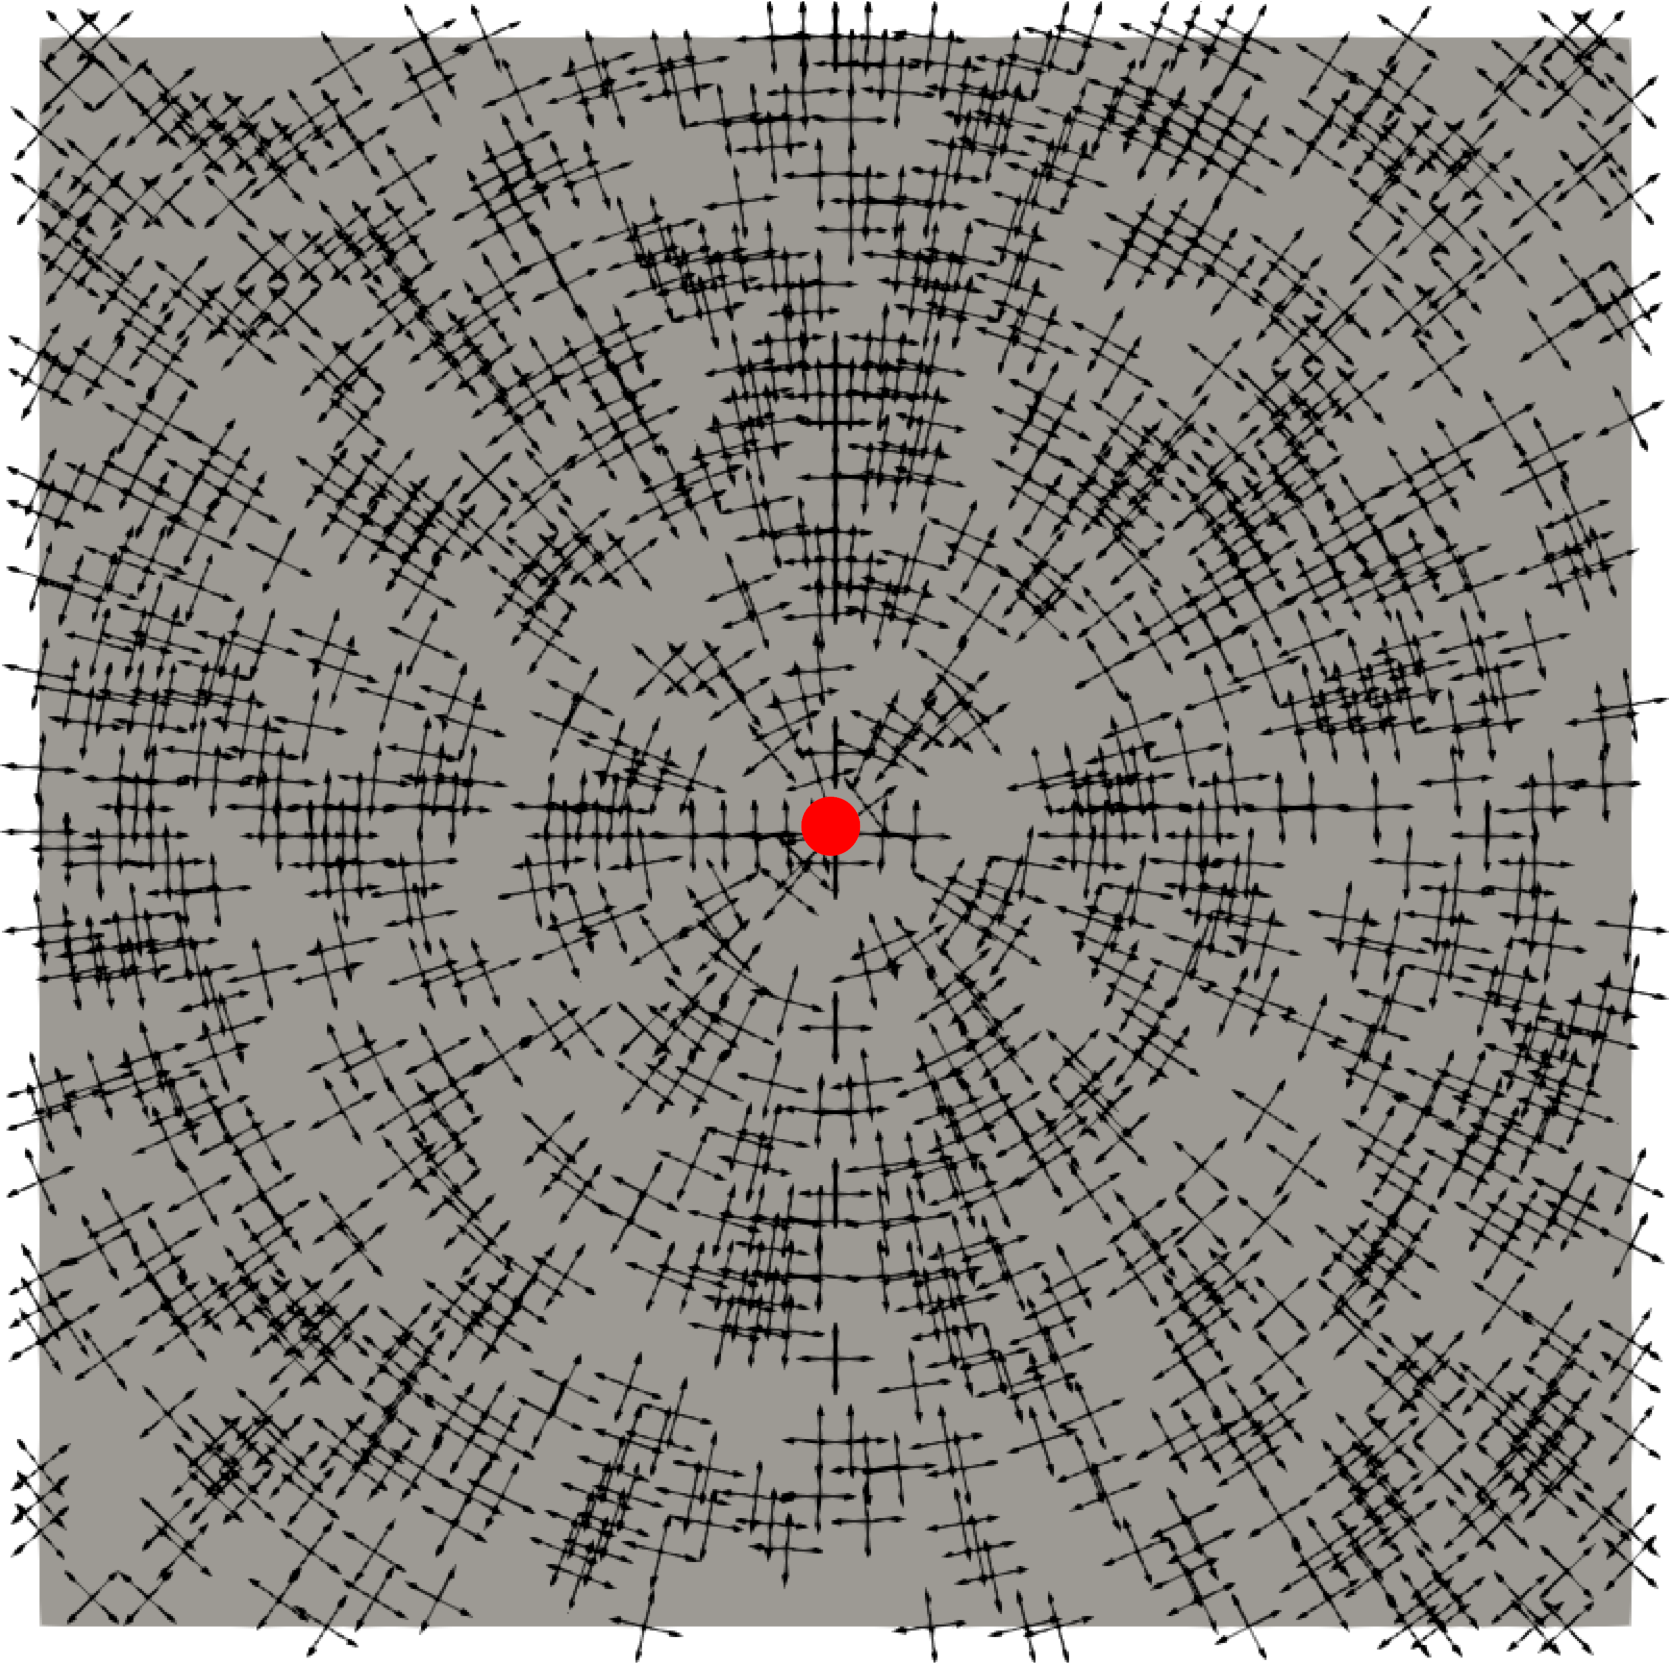
\includegraphics[scale=0.27]{images/u_sing.pdf}\hspace{0.2cm}
  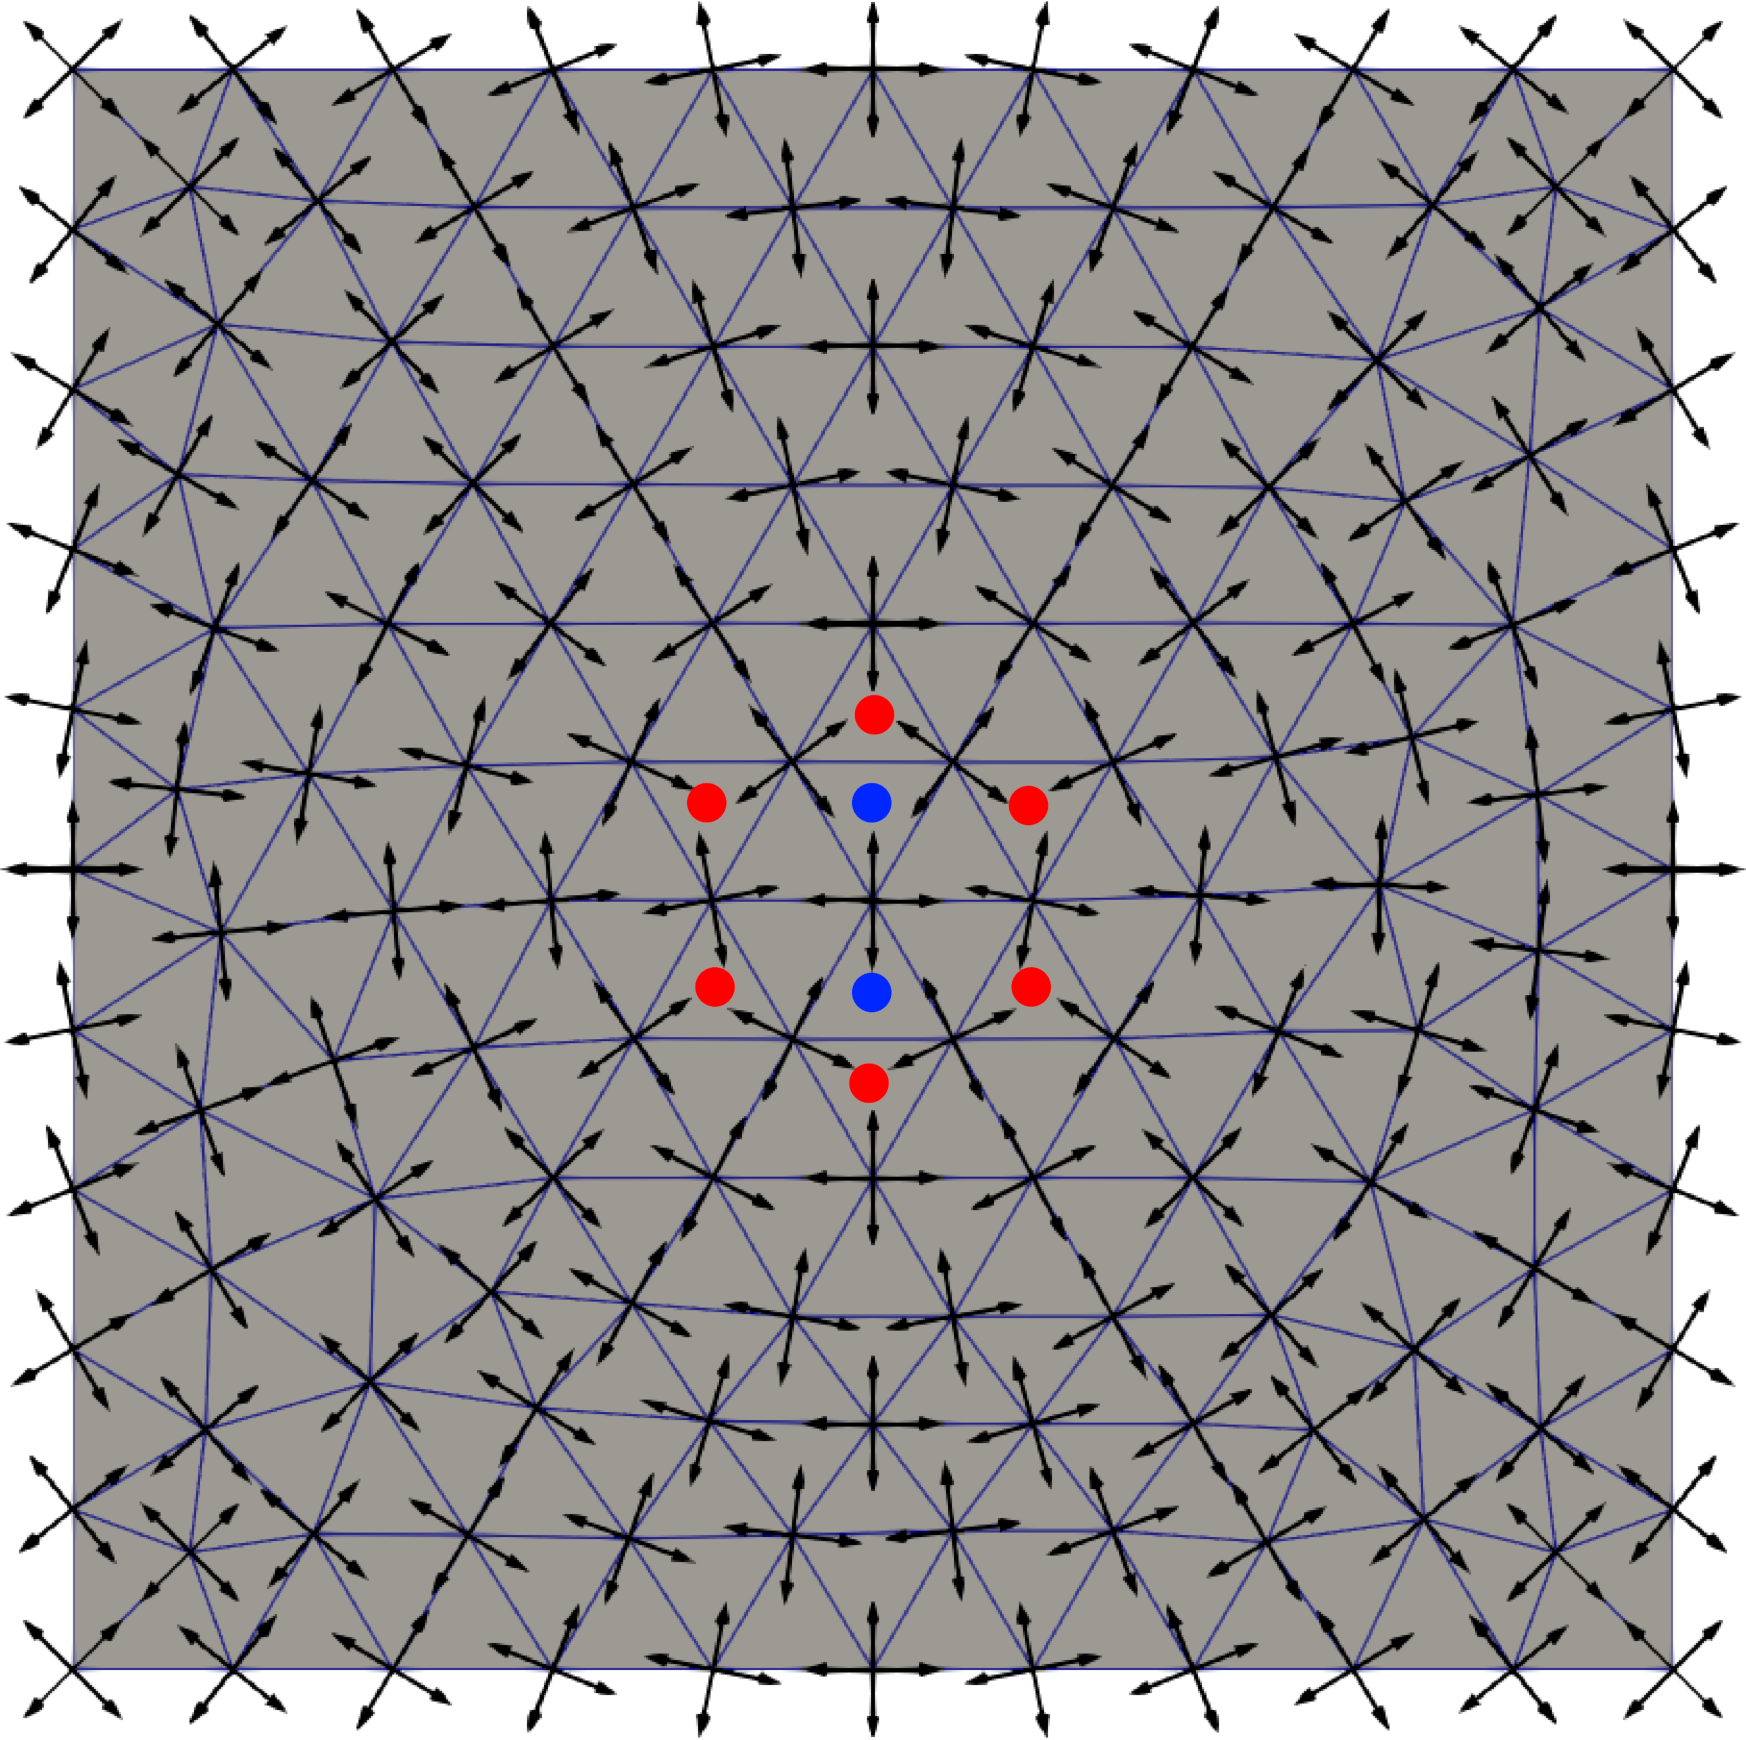
\includegraphics[scale=0.26]{images/u_h_sing.pdf}
  \caption{Gauche: Illustration des séparatrices émanant de points singuliers d'indice $-1/4$ (à gauche) et d'indice $1/4$ (à droite).}
  \label{fig:separatrice_illustration}
\end{figure}

\section{Partitionnement de $\partial\Omega_h$}

L'adaptation de l'algorithme de partitionnement \ref{alg:algo_main} au maillage $\Omega_h$ est donné par:\\

\begin{algorithm}[H]
\label{alg:discr_algo_main}
\SetKwInOut{Input}{Entrée}
\SetKwInOut{Output}{Sortie}
\Input{$\Omega_h$ un maillage triangulaire, champ de croix $\bar{u}_h$ linéaire par morceau sur chaque triangle de $\Omega_h$.}
\Output{Partition de $\Omega_h$ en ensembles de régions.}
\vspace{0.2cm}
1.) Identification des points singuliers du champ de croix,\\\vspace{0.2cm}
2.) Détermination du nombre de séparatrices pour chaque point singulier,\\\vspace{0.2cm}
3.) Intégration des séparatrices,\\\vspace{0.2cm}
4.) Identification des régions.\\\vspace{0.2cm}
\caption{Algorithme de partitionnement $\Omega_h$}
\end{algorithm}
\vspace{0.5cm}
On considère que l'algorithme a convergé si les séparatrices ne convergent pas vers un cycle limite. Examinons maintenant en détail certaines étapes de cet algorithme:

\subsection{Recherche de points singuliers}

Par construction, les points singuliers du champ de croix $\bar{u}_h$ se situent soit aux sommets du maillage $\Omega_h$, soit à l'intérieur des triangles qui le constituent.En pratique, la recherche de ces points peut être effectuée localement sur chaque triangle. Cela implique de tester le caractère singulier ou non de chaque triangle (voir la définition \ref{def:triangle_singulier}). Considérons $T\in\mathcal{T}_h$ comme un triangle singulier de $\Omega_h$. Par conception, il contient nécessairement un point singulier. Nous distinguons alors deux cas :\\
\begin{itemize}
 \item le point singulier correspond à l'un des sommets du triangle $T$.\\
 \item sinon, le point singulier se trouve à l'intérieur du triangle. Conformément à notre représentation de $\bar{u}_h$, dans ce cas précis, il s'agit du barycentre du triangle. Cependant rien empêche de choisir un autre point à l'intérieur du triangle tout en modifiant le calcul des valeurs du champ dans le triangle. Remarquons que tous les points singuliers de bord sont sur des sommets.\\
\end{itemize}

Une fois la localisation des points singulier identifié, on peut facilement calculé leur index grâce aux formules \ref{eqn:ind_int} ou \ref{eqn:ind_bord} en fonction de leur localisation.

\begin{remark}
    Grace à la proposition on peut chosir l'emplacement du point singulier dans $T_p$. en l'occurence, pour ne pas avoir à en faire la recherche on peut choisir le barycentre du triangle.\\
\end{remark}


On peut rasssembler plusieurs singularité voisine en une.. permet d'éviter les problématiques de point trop proche par exemple.
Illustrer tout ça 


\subsection{Construction des séparatrices}

Une fois les points singuliers de $\bar{u}_h$ identifiés, nous procédons à la création des séparatrices sur $\Omega_h$. Cette étape comprend le calcul du nombre de séparatrices à assigner à chaque point singulier, la détermination des directions initiales pour chaque séparatrice, ainsi que l'intégration de ces séparatrices.

\paragraph{Nombre de séparatrices:} Si $p$ est un point singulier de $\bar{u}_h$, alors le nombre de séparatrices $N_s(p)$ associées à $p$ est donné par:
\begin{equation}
    N_s(p) = 
    \left\{
    \begin{array}{ll}
    4-4id_{\bar{u}_h}(p) & \mbox{ si } p\in\Omega_h\backslash\partial\Omega_h\\[0.3cm]
    2-4id_{\bar{u}_h}(p) & \mbox{ si } p\in\partial\Omega_h
    \end{array}
    \right.
\end{equation}

\paragraph{Directions initiales et intégration:}

Soit $p_0\in\mathcal{S}_{\bar{u}_h}\backslash\partial\Omega_h$. Étant donné que $\bar{u}_h$ s'annule en $p_0$, notre première étape consiste à déterminer les orientations initiales des séparatrices. Les directions initiales des séparatrices émanant de $p_0$ sont données par les vecteurs $\overrightarrow{p_0q_i}$, $i\in\llbracket 1, N_s(p_0) \rrbracket$ où la suite de points $(q_i)_{i\in\llbracket 1, N_s(p_0)\rrbracket}\subset\partial T_{p_0}$ est construite de la manière suivante (voir figure \ref{fig:init_streams_int}):\\
\begin{itemize}
    \item[$\bullet$] le premier point $q_1$ est tout point de $\partial T_{p_0}$ tel que $\overrightarrow{p_0q_1}.\|\overrightarrow{p_0q_1}\|^{-1}\in\bar{u}_h(q_1)$\\
    \item[$\bullet$] soit $t_1\in[0, 1]$ tel que $\gamma(t_1)=q_1$. Pour tout $i\in\llbracket 2, N_s(p_0)\rrbracket$, on a:
    $$
    q_i=\gamma(t_i)\mbox{ avec }\int_{t_{i-1}}^{t_i}dW_{p_0}^\gamma=-\frac{\pi}{2},
    $$
    où $\gamma$ est une paramétrisation de $\partial T_{p_0}$ sur $[0, 1]$ dans le sens positif et la fonction $W^\gamma_{p_0}$ est donné pour tout $t\in[0, 1]$ par:
    $$
    W_{p_0}^\gamma(t)=\theta^\gamma_{\bar{u}_h}(t)-\arg \overrightarrow{p_0\gamma(t)}.
    $$

    \begin{figure}[!h]
    \centering
    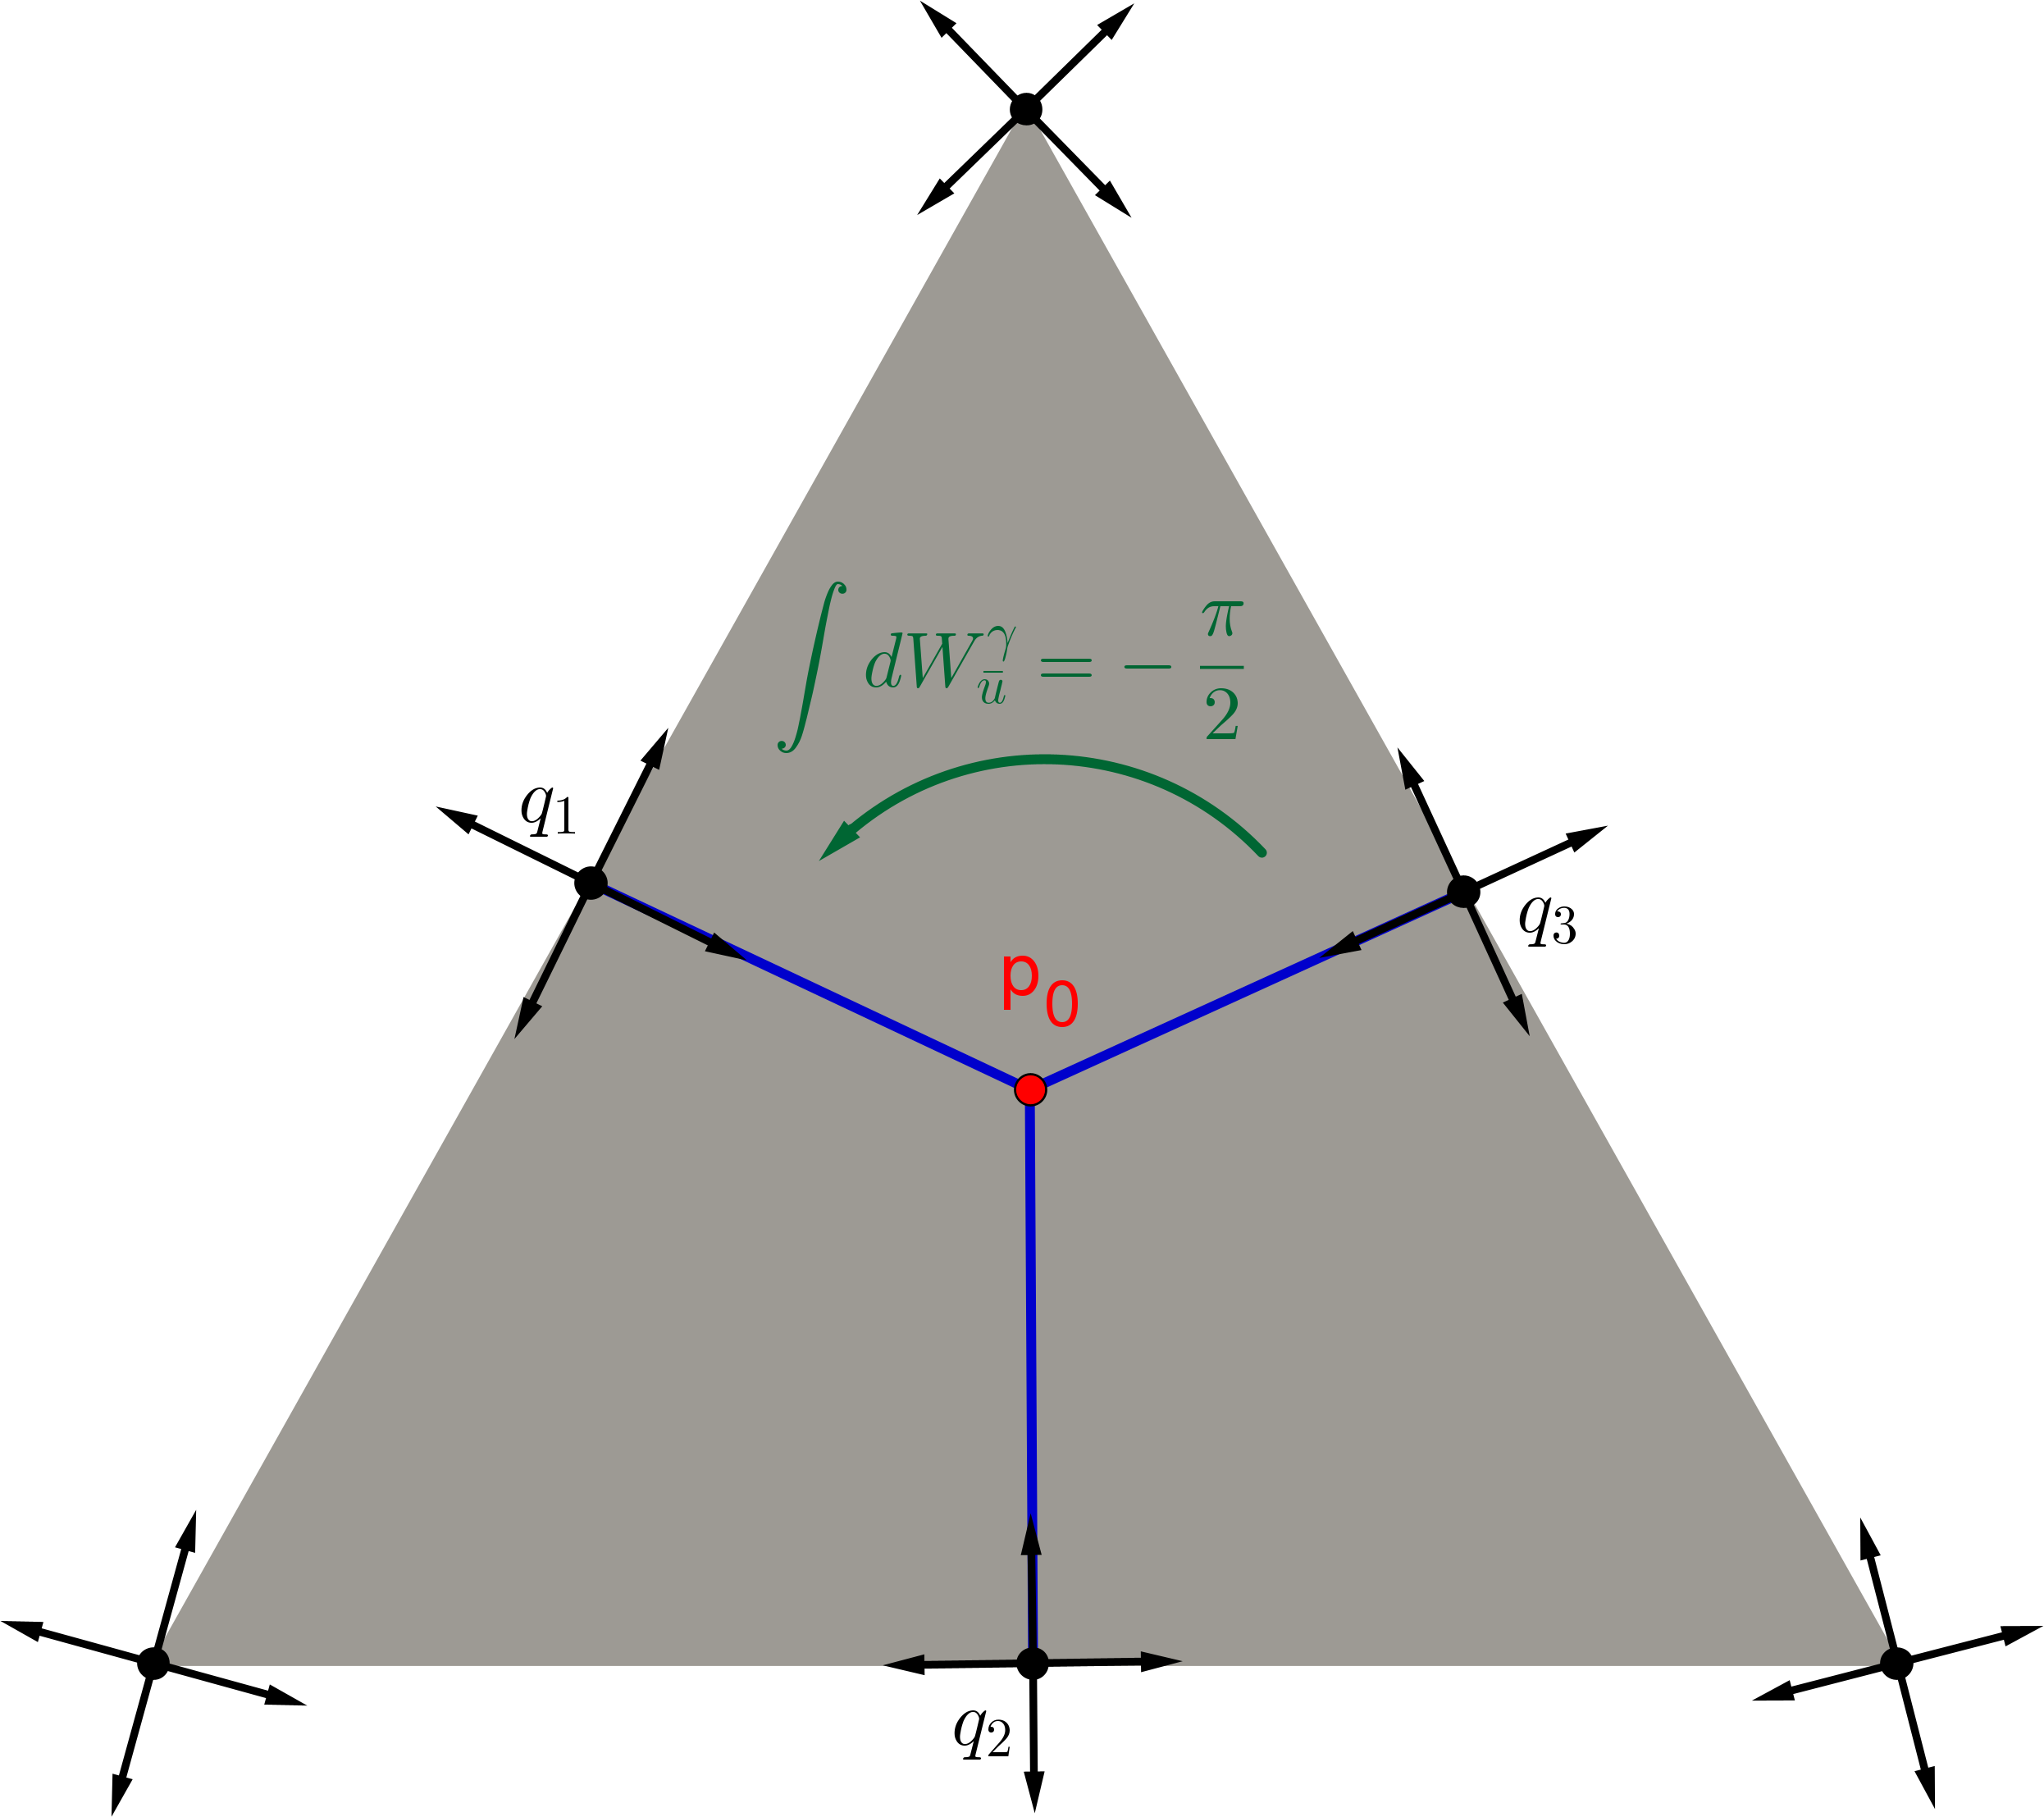
\includegraphics[scale=0.755]{images/triangle separatrices 3.png}
    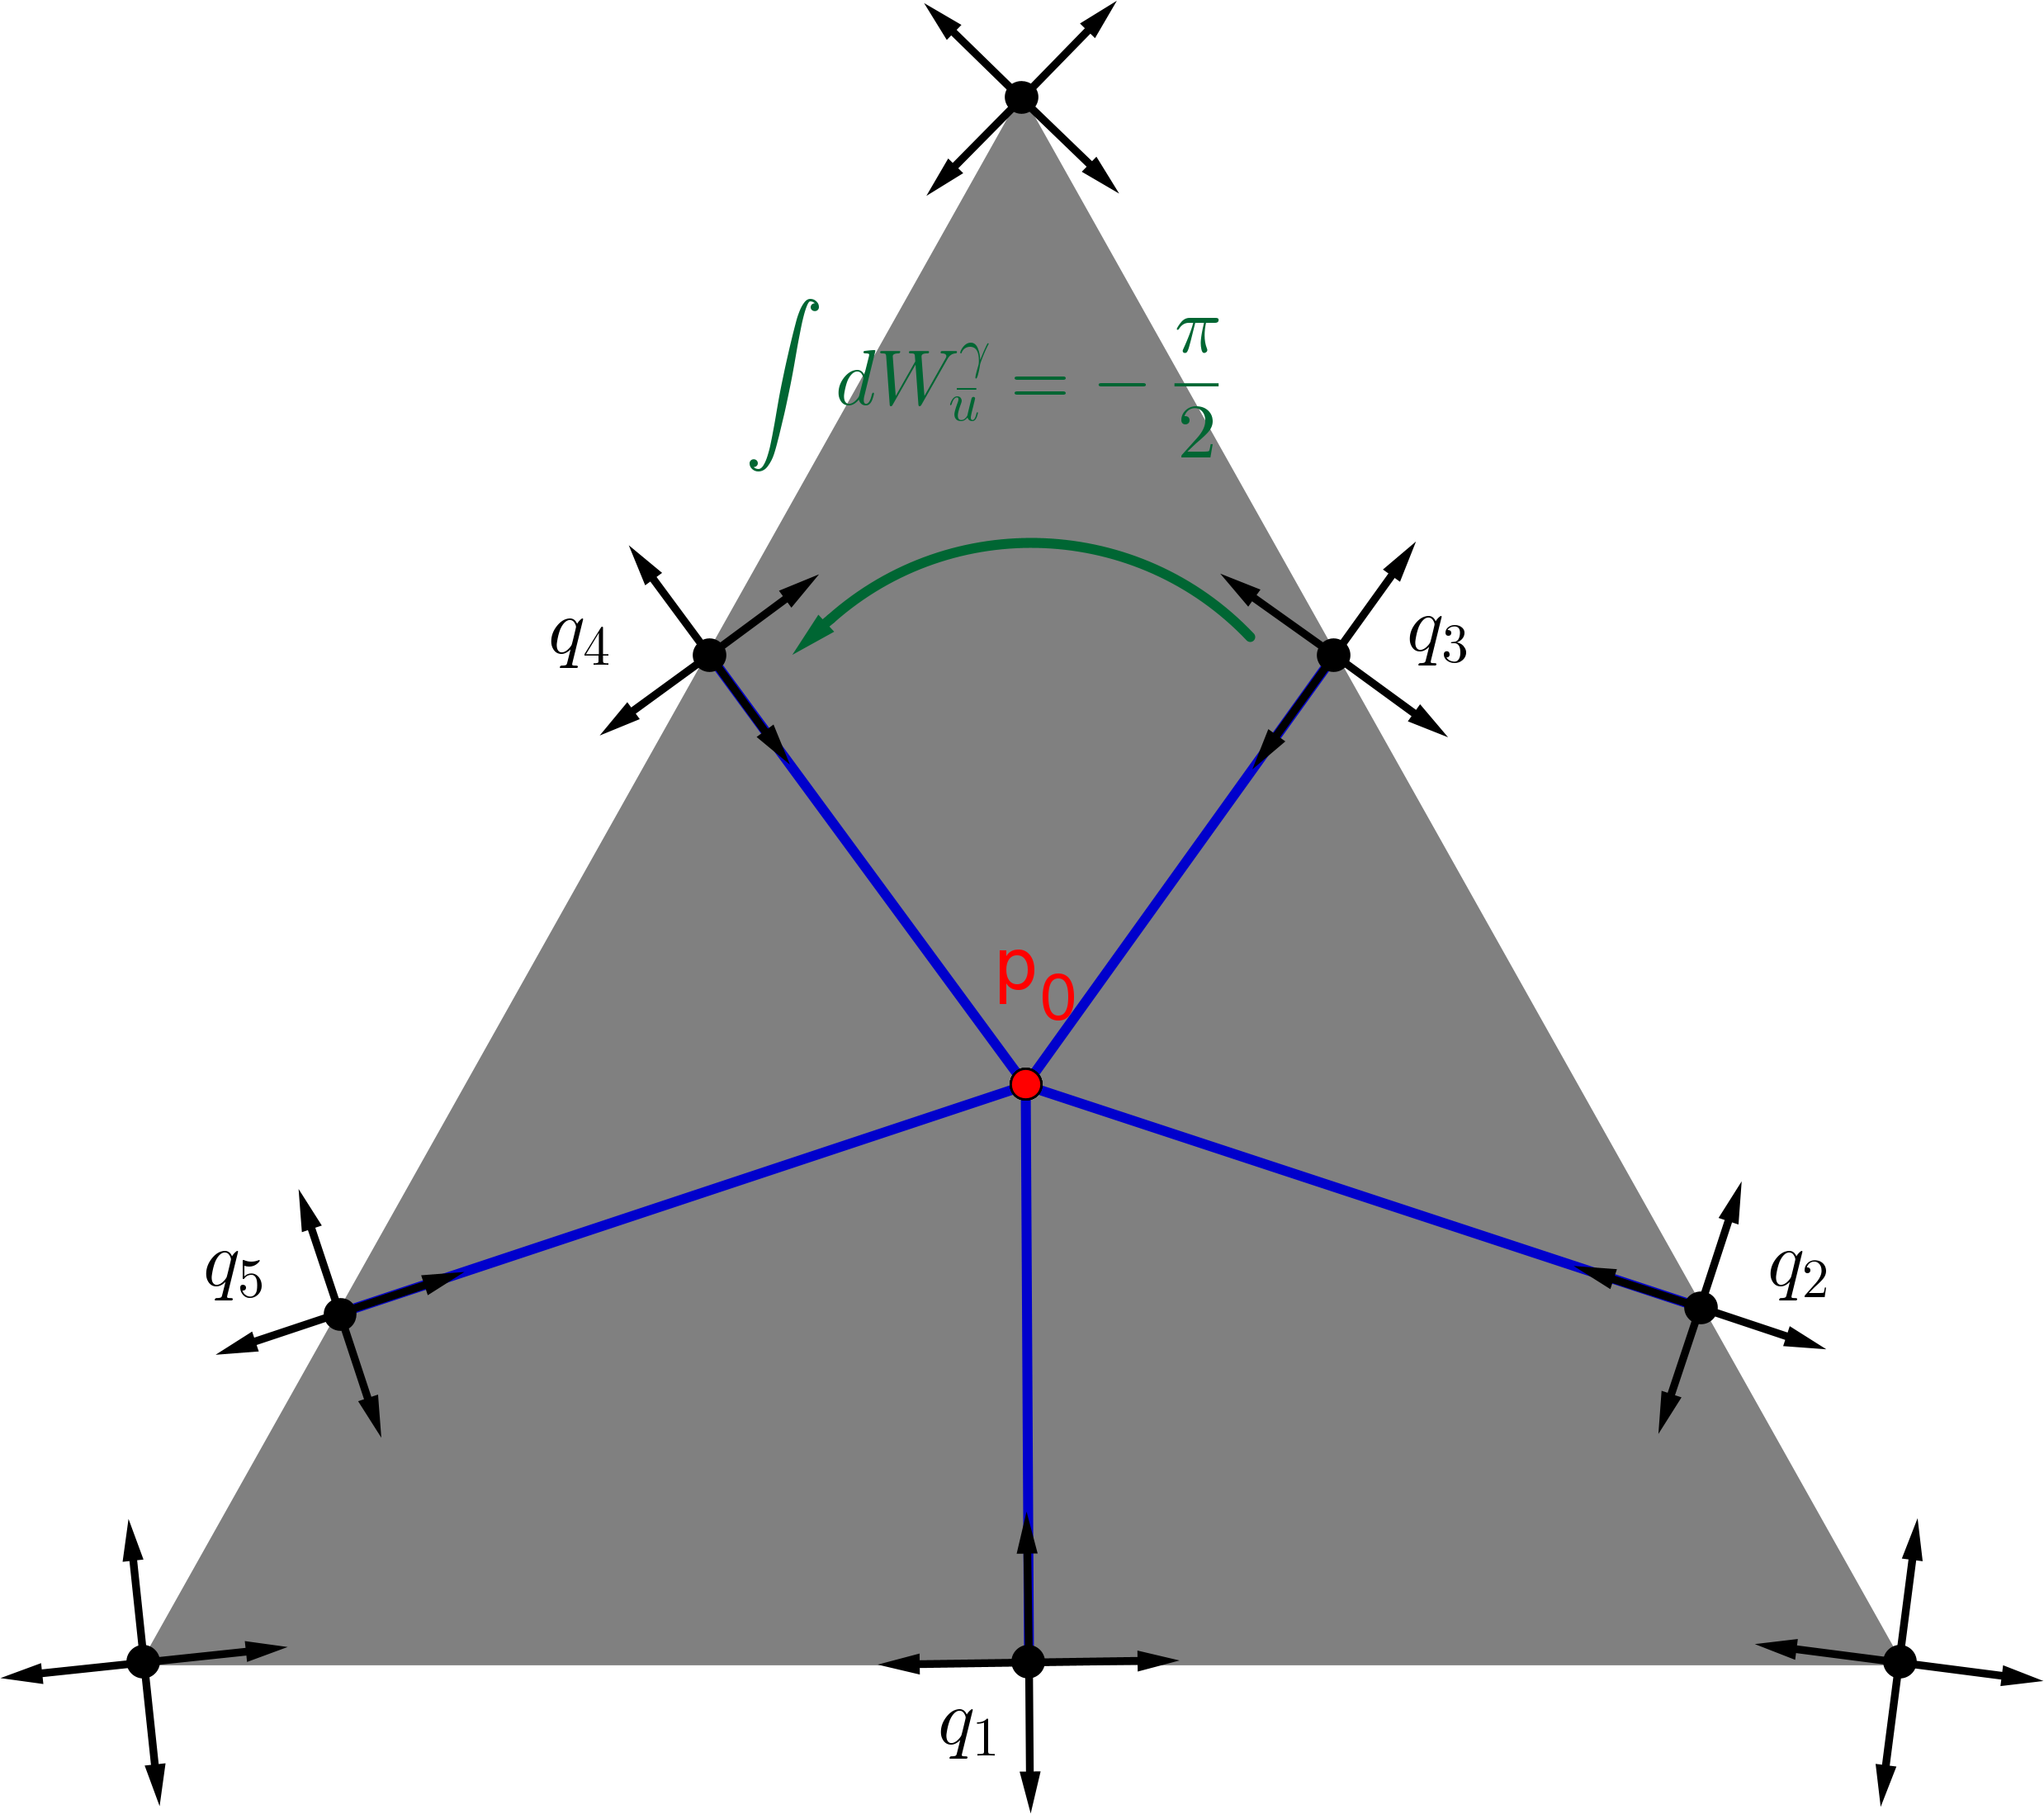
\includegraphics[scale=0.755]{images/triangle separatrices 5.png}
    \caption{Illustration du maillage quadrilatéral d'un anneau à partir d'un champ de croix radial.}
    \label{fig:init_streams_int}
    \end{figure}
\end{itemize}

Si $p_0\in\mathcal{S}_{\bar{u}_h}\cap\partial\Omega_h$ alors

\begin{figure}[!h]
\centering
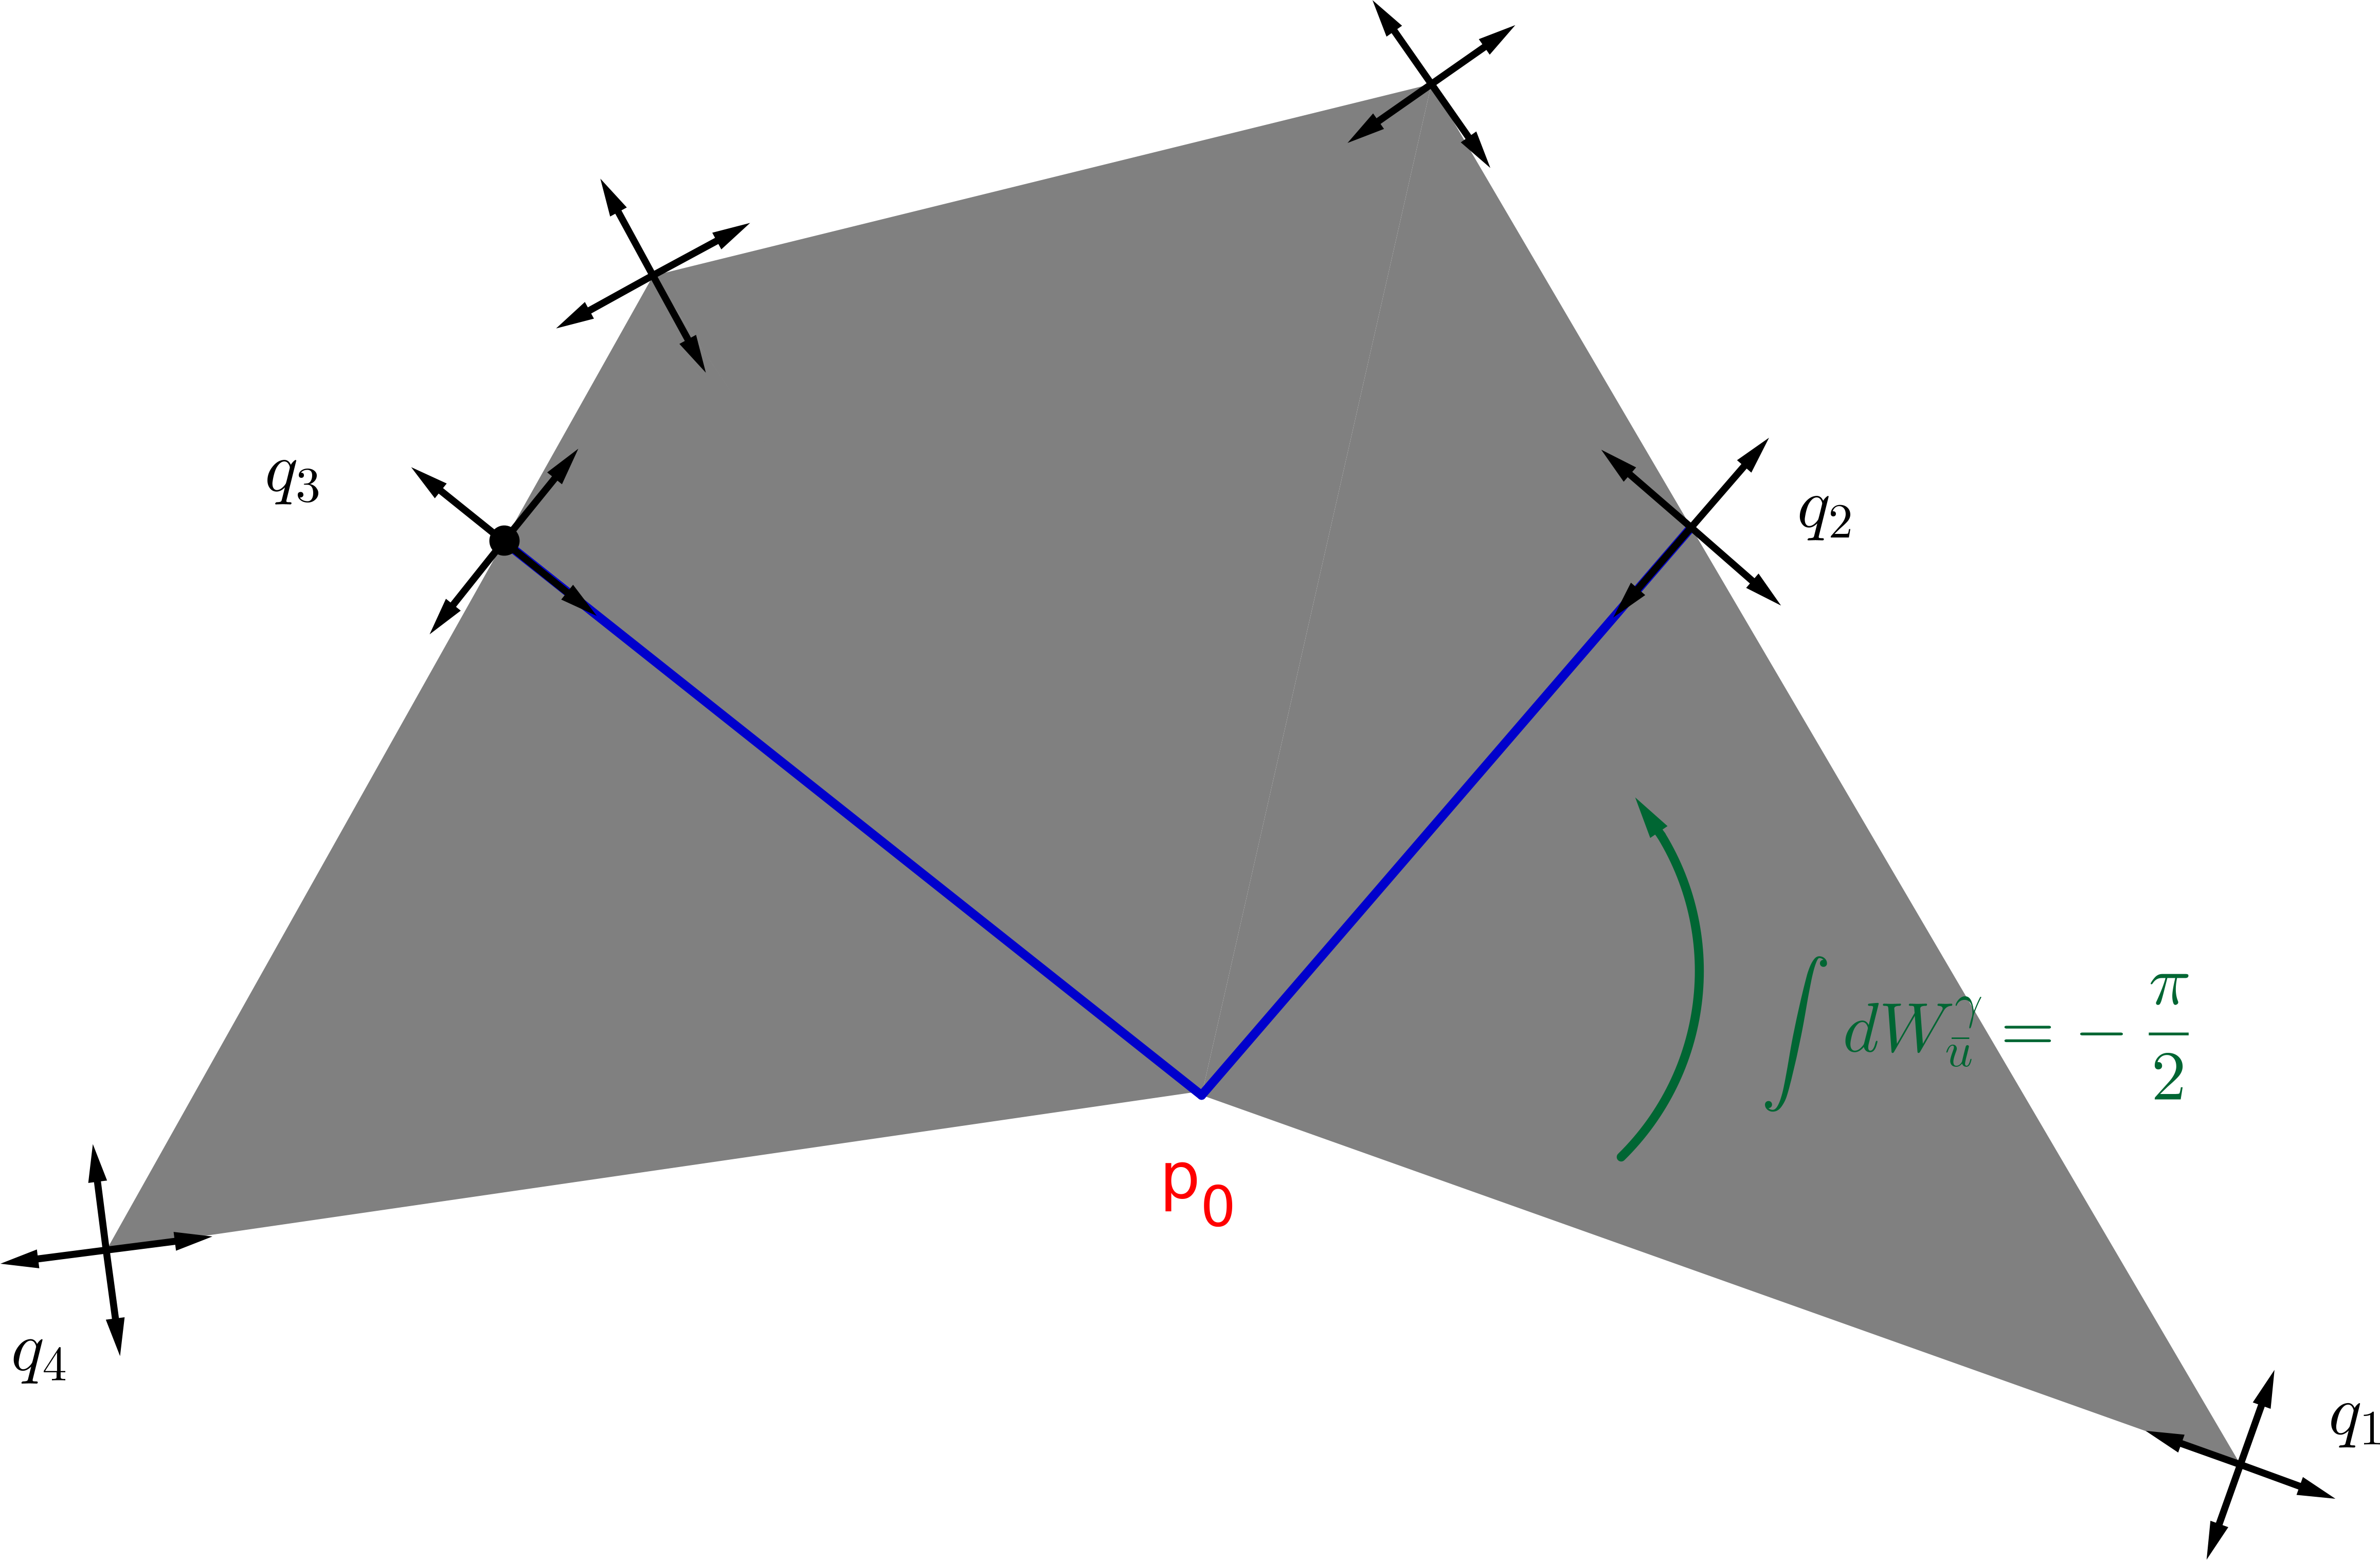
\includegraphics[scale=0.755]{images/triangle separatrices bord.png}
\caption{Illustration du maillage quadrilatéral d'un anneau à partir d'un champ de croix radial.}
\label{fig:init_streams_bord}
\end{figure}

\[\]

direction de sortie mieux chez moi que chez les autres

\begin{figure}[!h]
\centering
\begin{subfigure}{0.65\textwidth}
    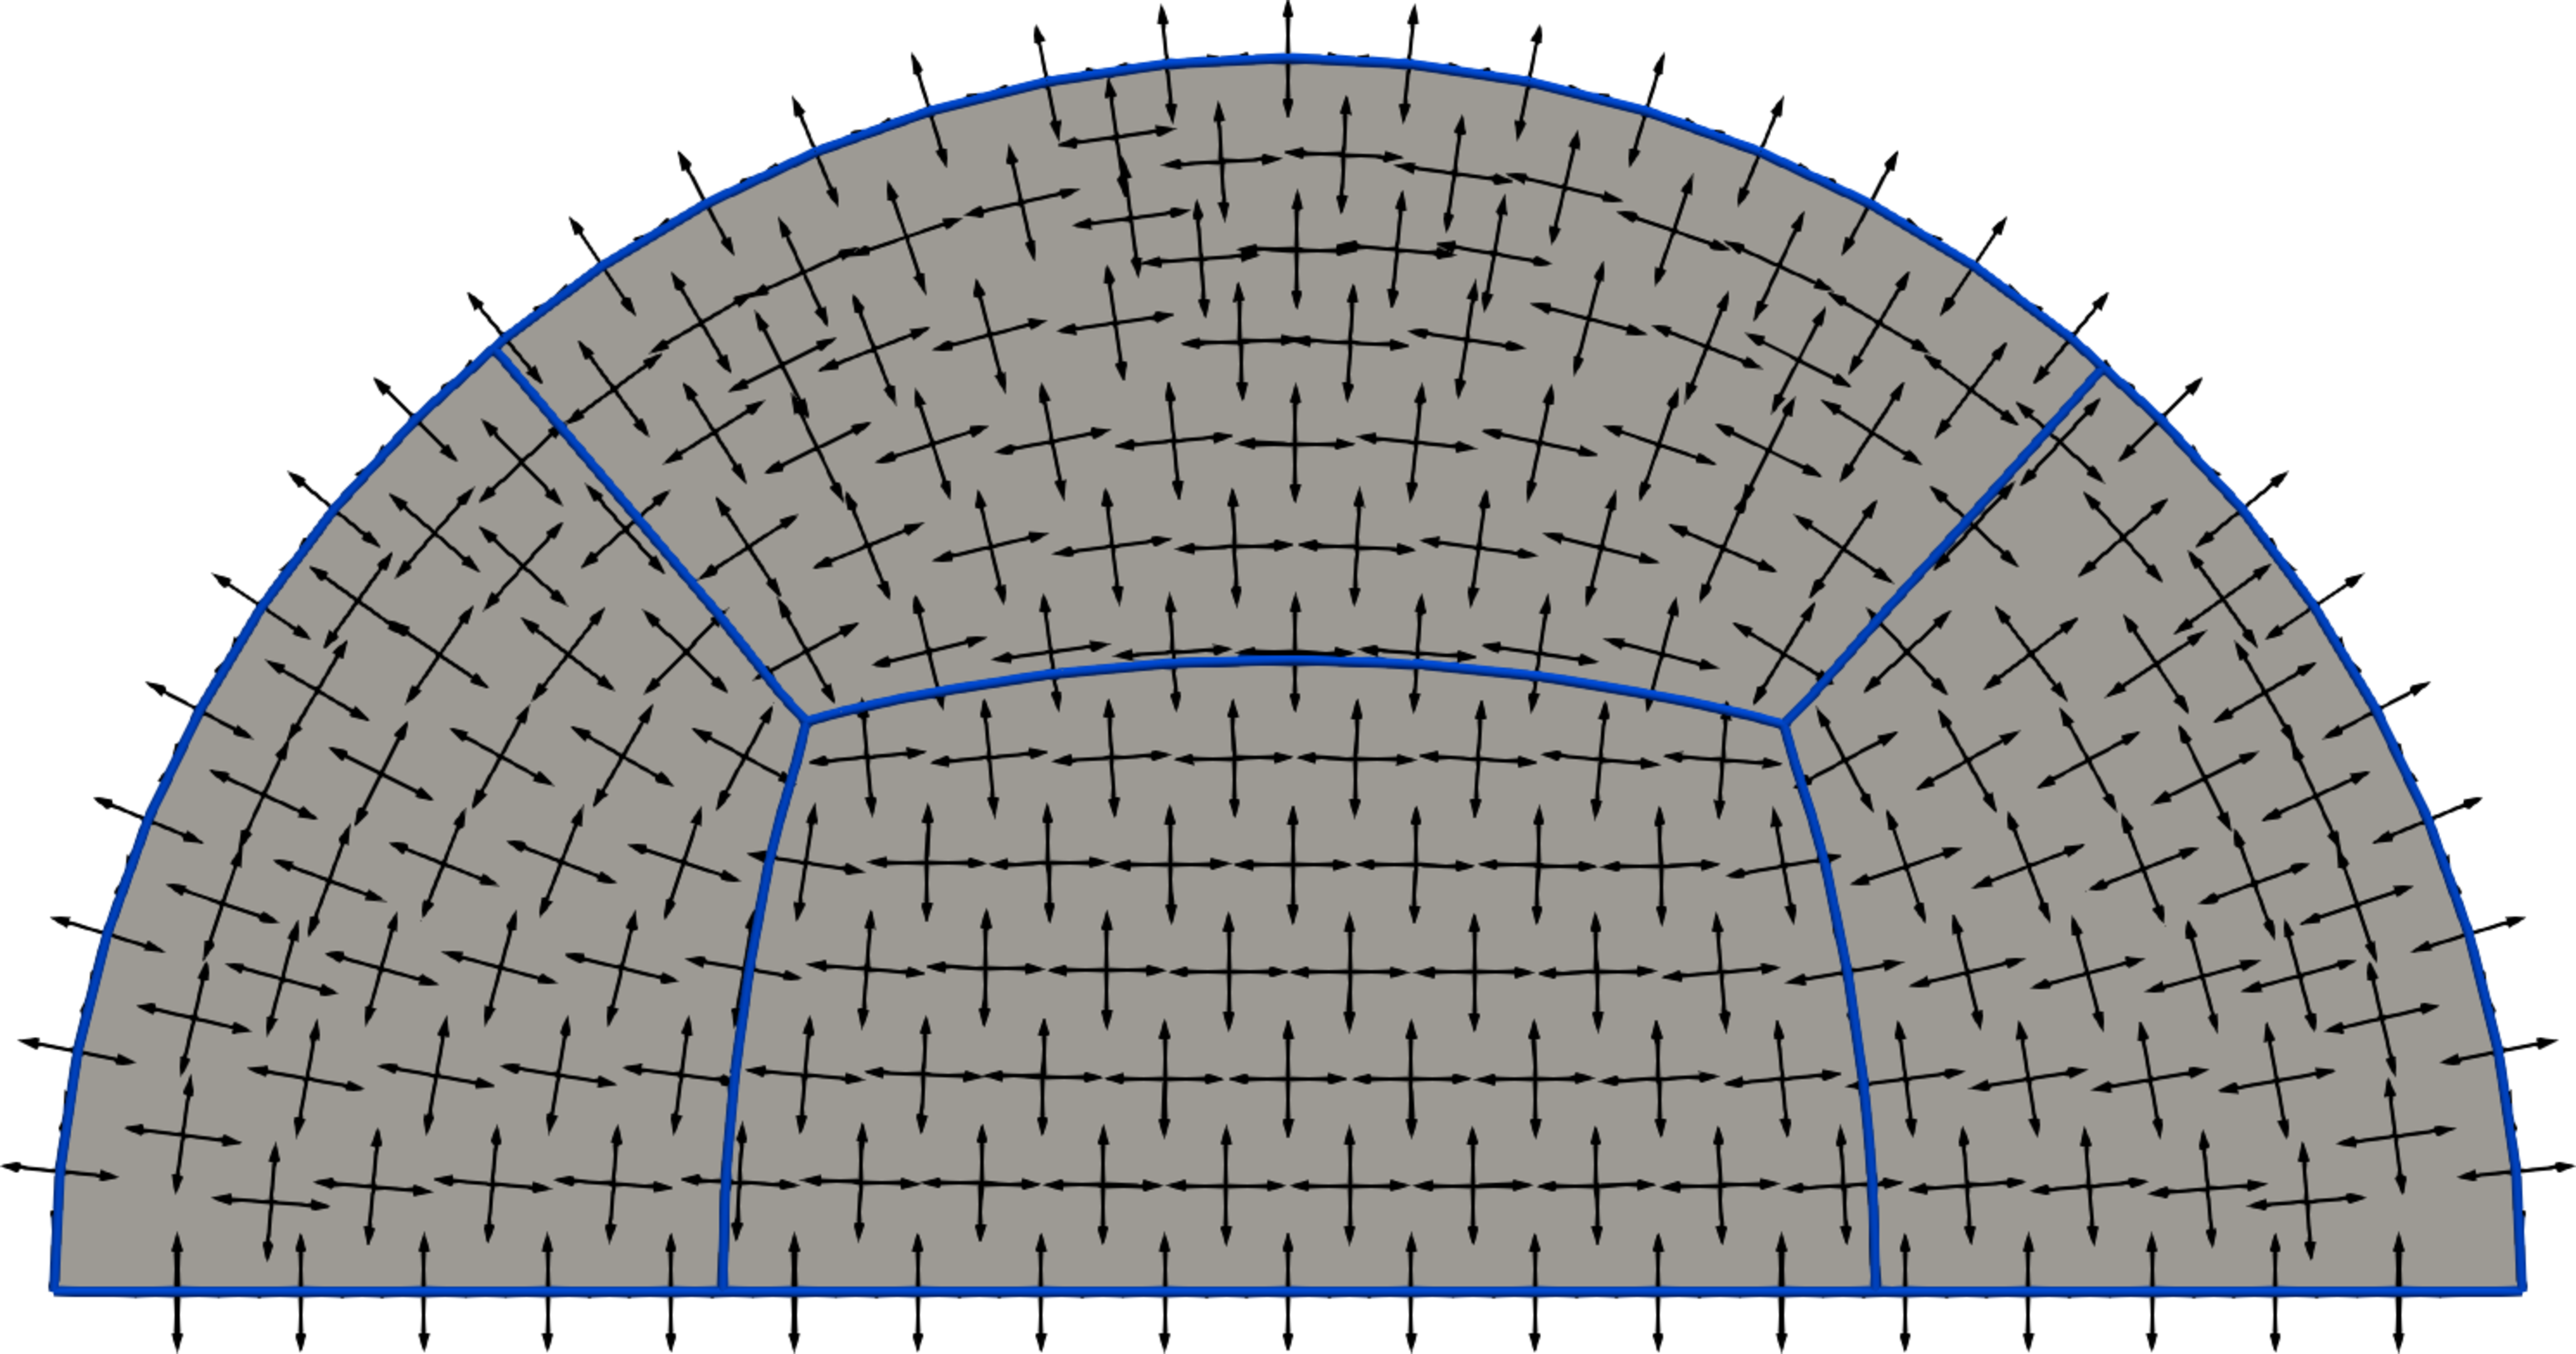
\includegraphics[width=\textwidth]{images/demi_disc_second_phi_first.pdf}
    \caption{Alignement du champ de croix présenté sur la figure \ref{fig:demiDisc_valProp_mauvaix_decoup} sur le bord du domaine et partitionnement du domaine.}
    \label{fig:first_dir_first}
\end{subfigure}
\\[0.5cm]
\begin{subfigure}{0.65\textwidth}
    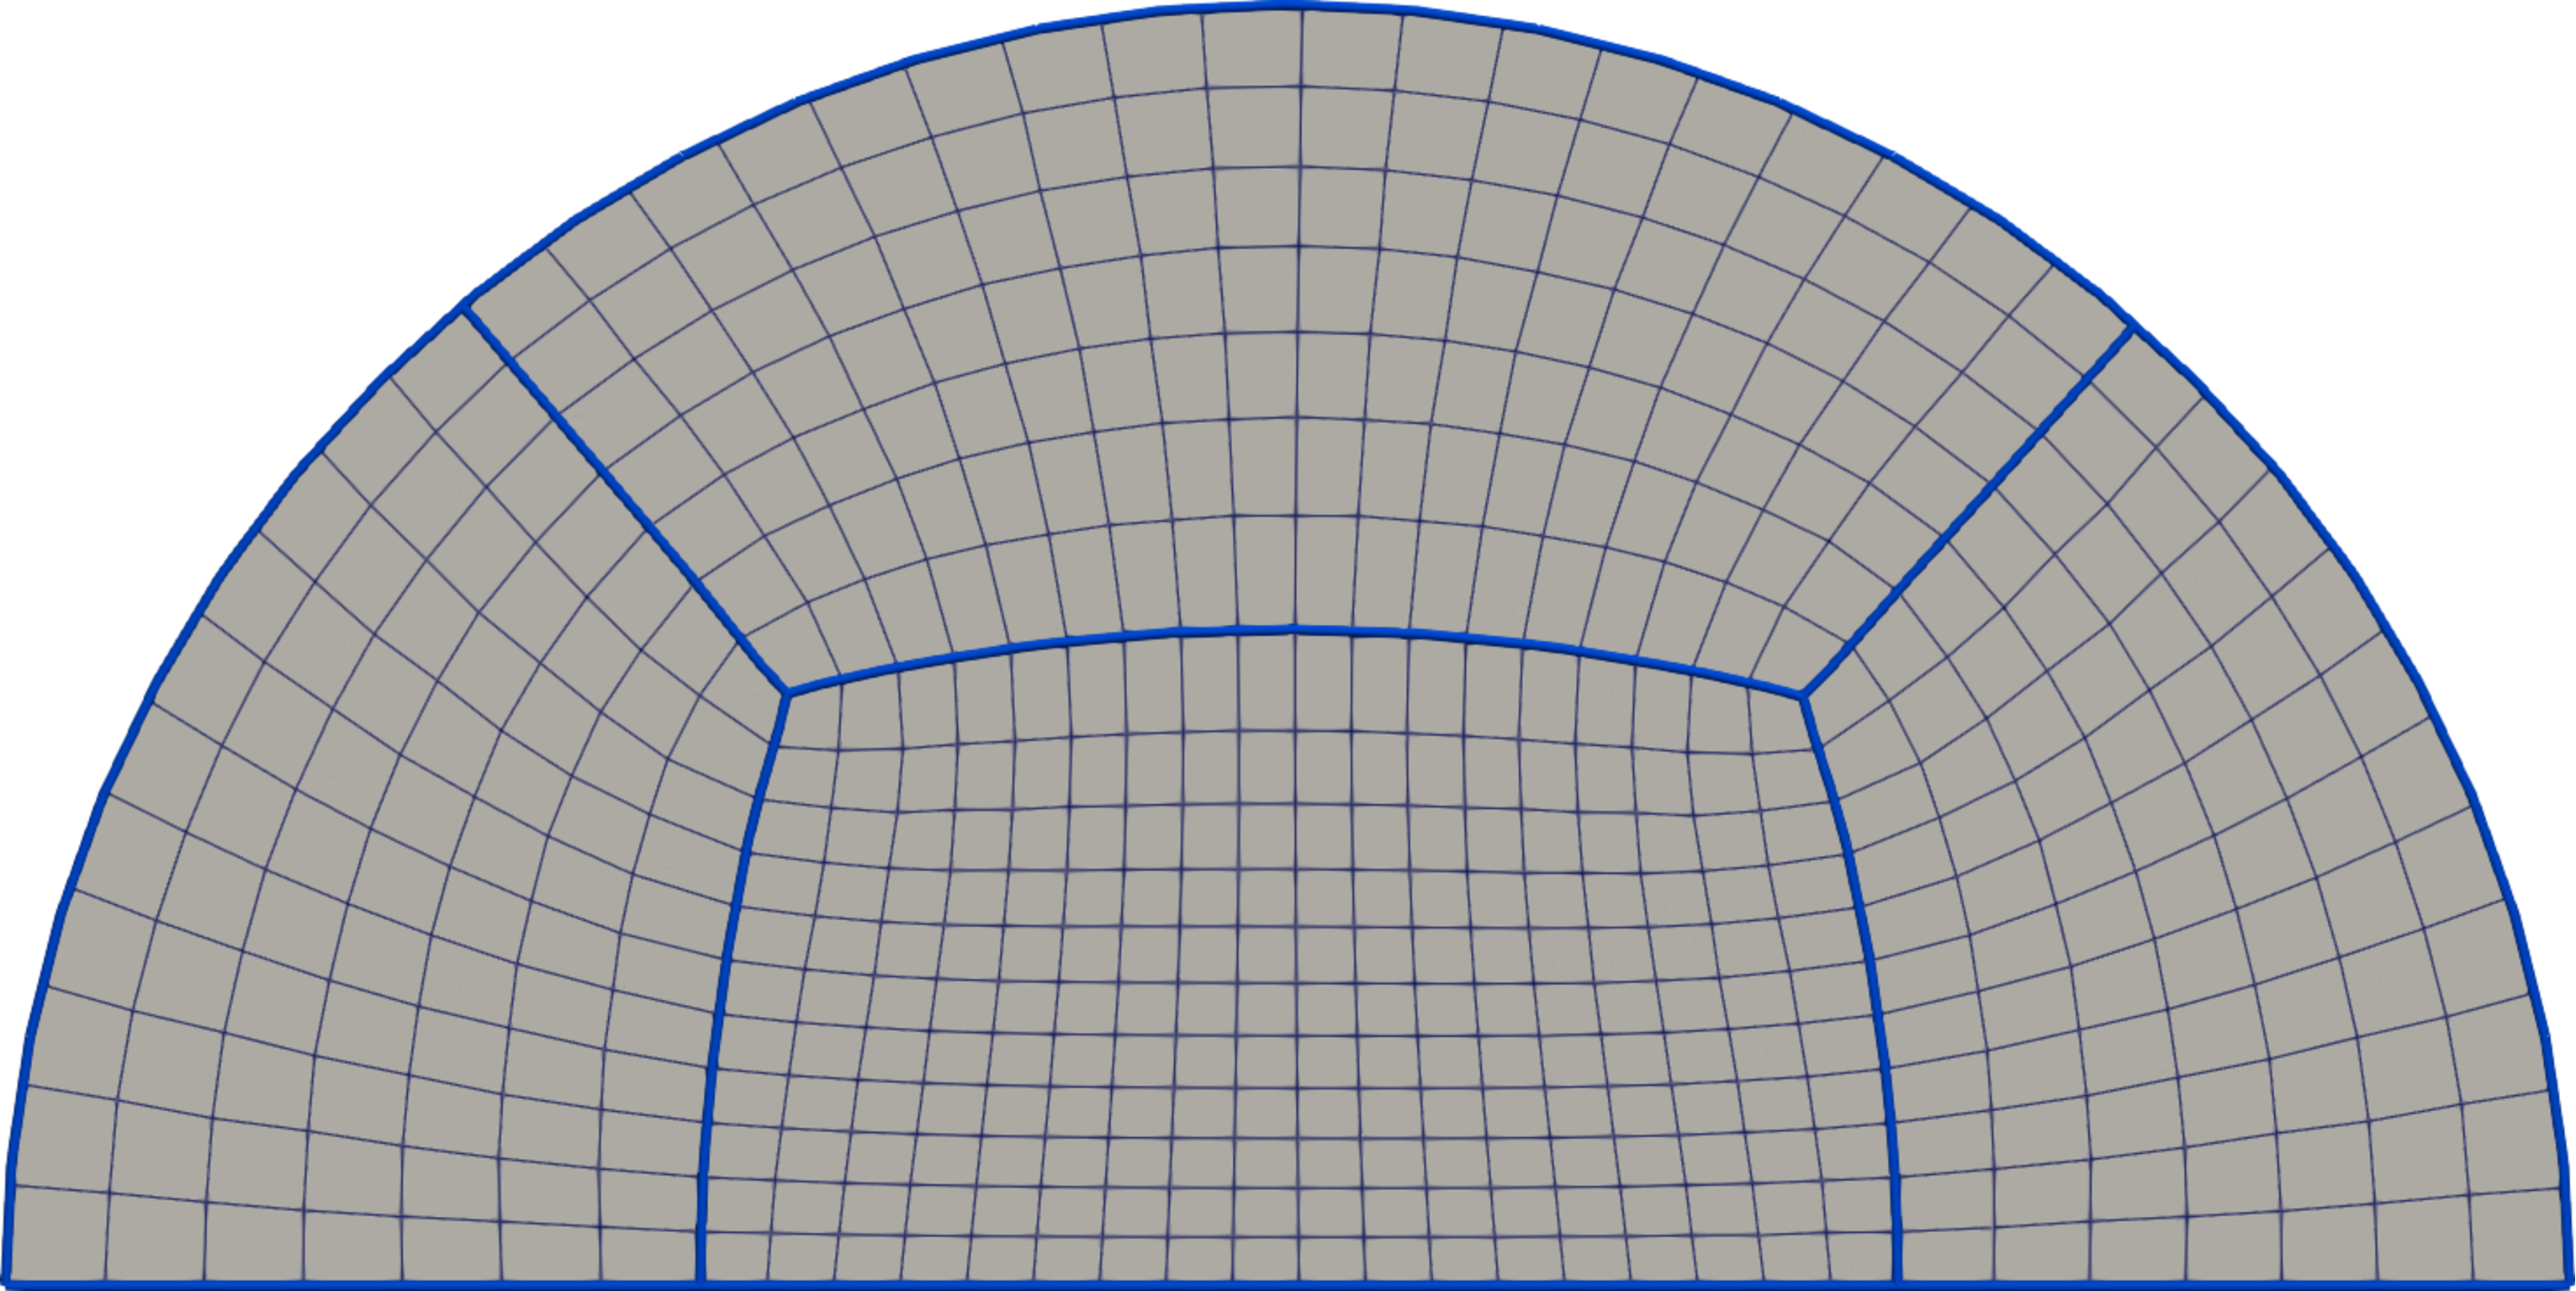
\includegraphics[width=\textwidth]{images/demi_disc_second_phi_second.pdf}
    \caption{Maillage quadrilatéral du domaine.}
    \label{fig:first_dir_second}
\end{subfigure}        
\caption{Direction de sortie différentes.}
\label{fig:first_dir}
\end{figure}


\paragraph{Traversé d'un triangle singulier:} lors de l'intégration d'une séparatrice, il peut arrivé que. lorsque le segment $[p_ip_{i+1}]$ traverse un triangle singulier, l'angle du champ varie beaucoup. On remplace alors le segment en question par une succecion d'autre segment calculé en raffinant localement le maillage dans le triangle singulier. L'idée est d'isoler le point singulier par rapport à la trajectoire de la séparatrice.

\begin{figure}[!h]
\centering
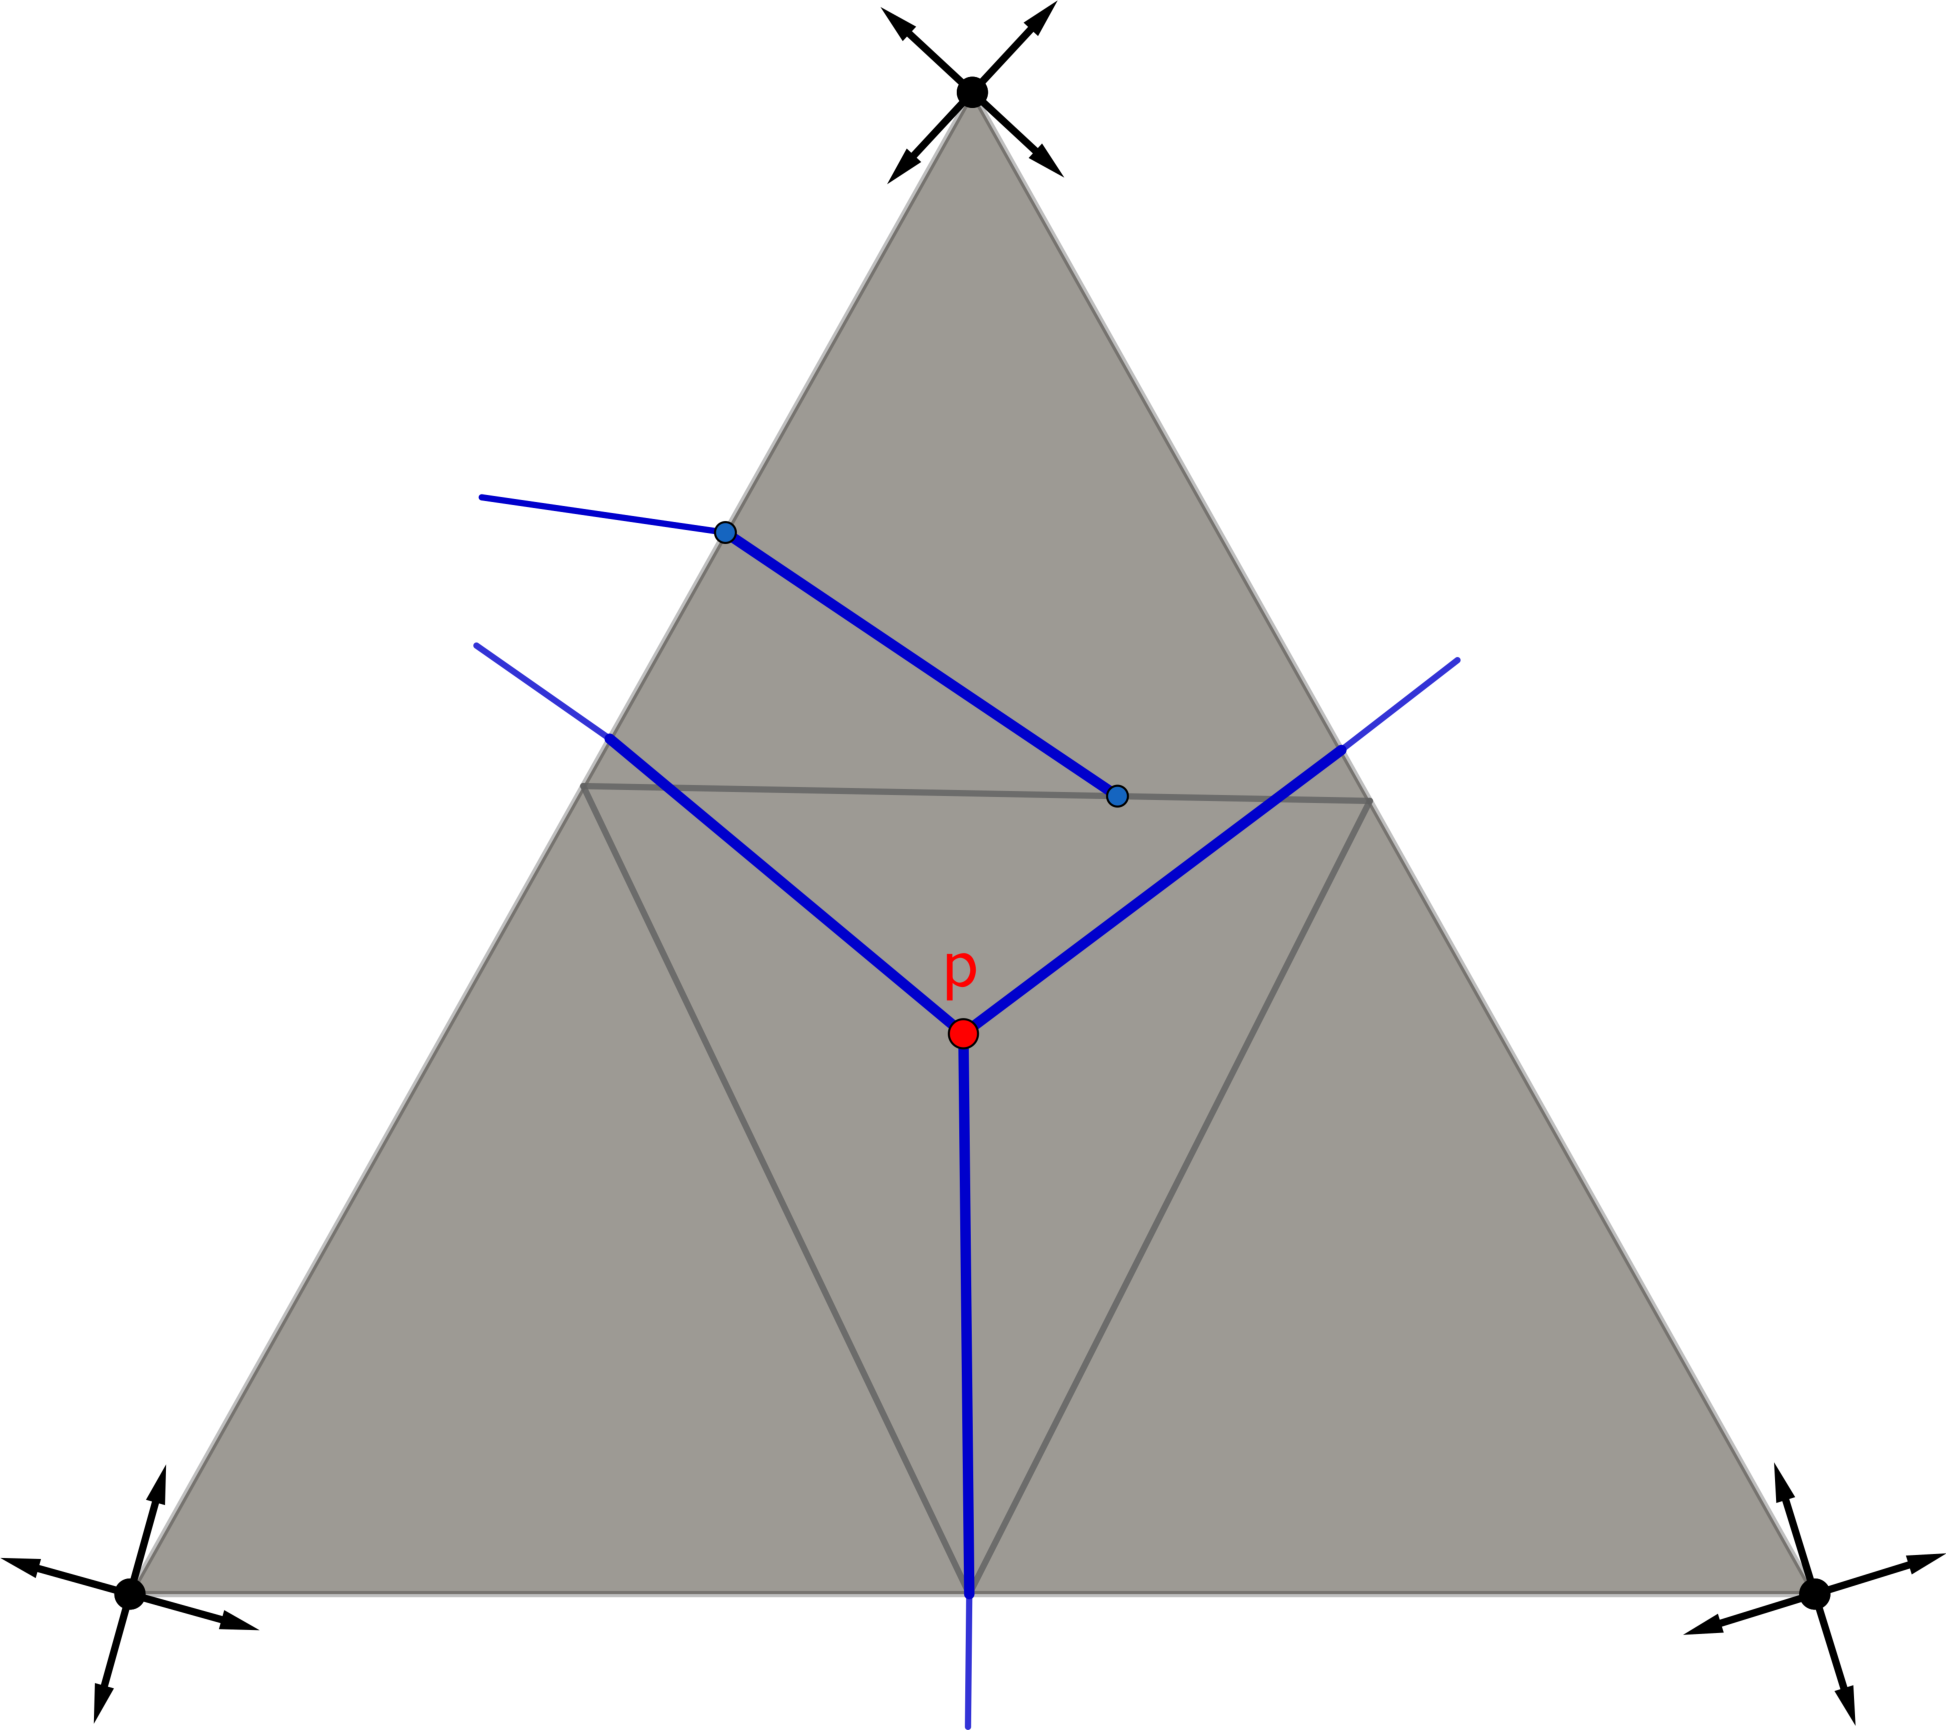
\includegraphics[scale=0.2]{images/draw_streams_sing_2.pdf}\hfill
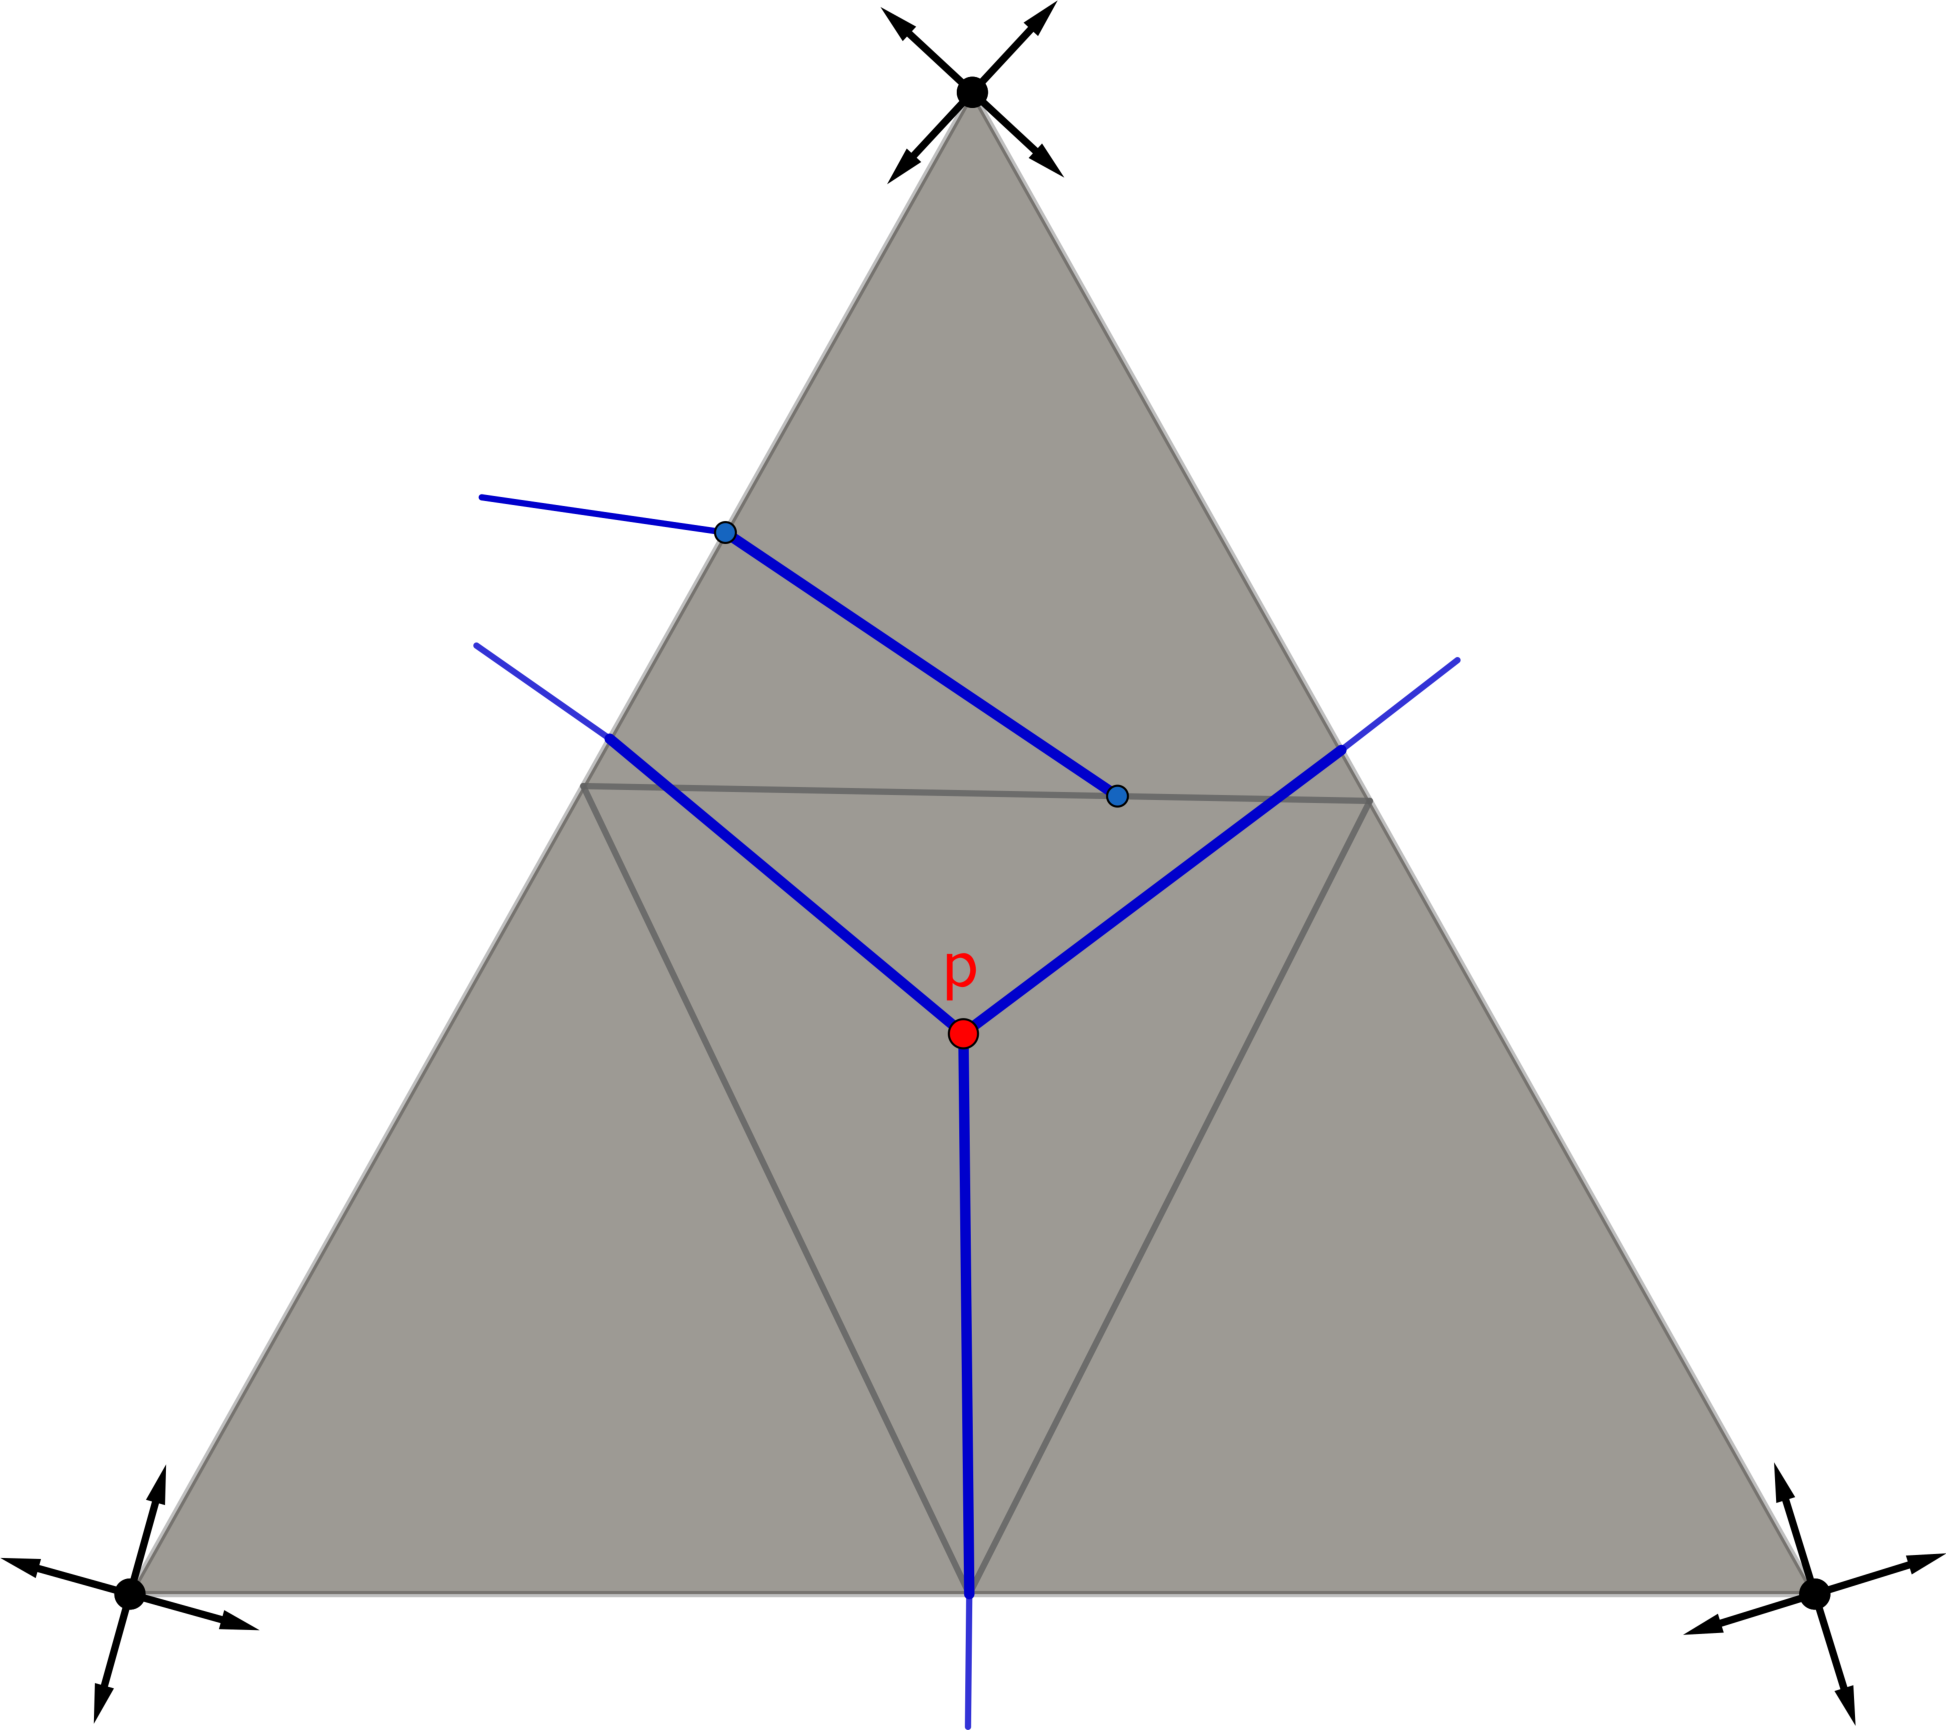
\includegraphics[scale=0.2]{images/draw_streams_sing_2.pdf}\vspace{1cm}
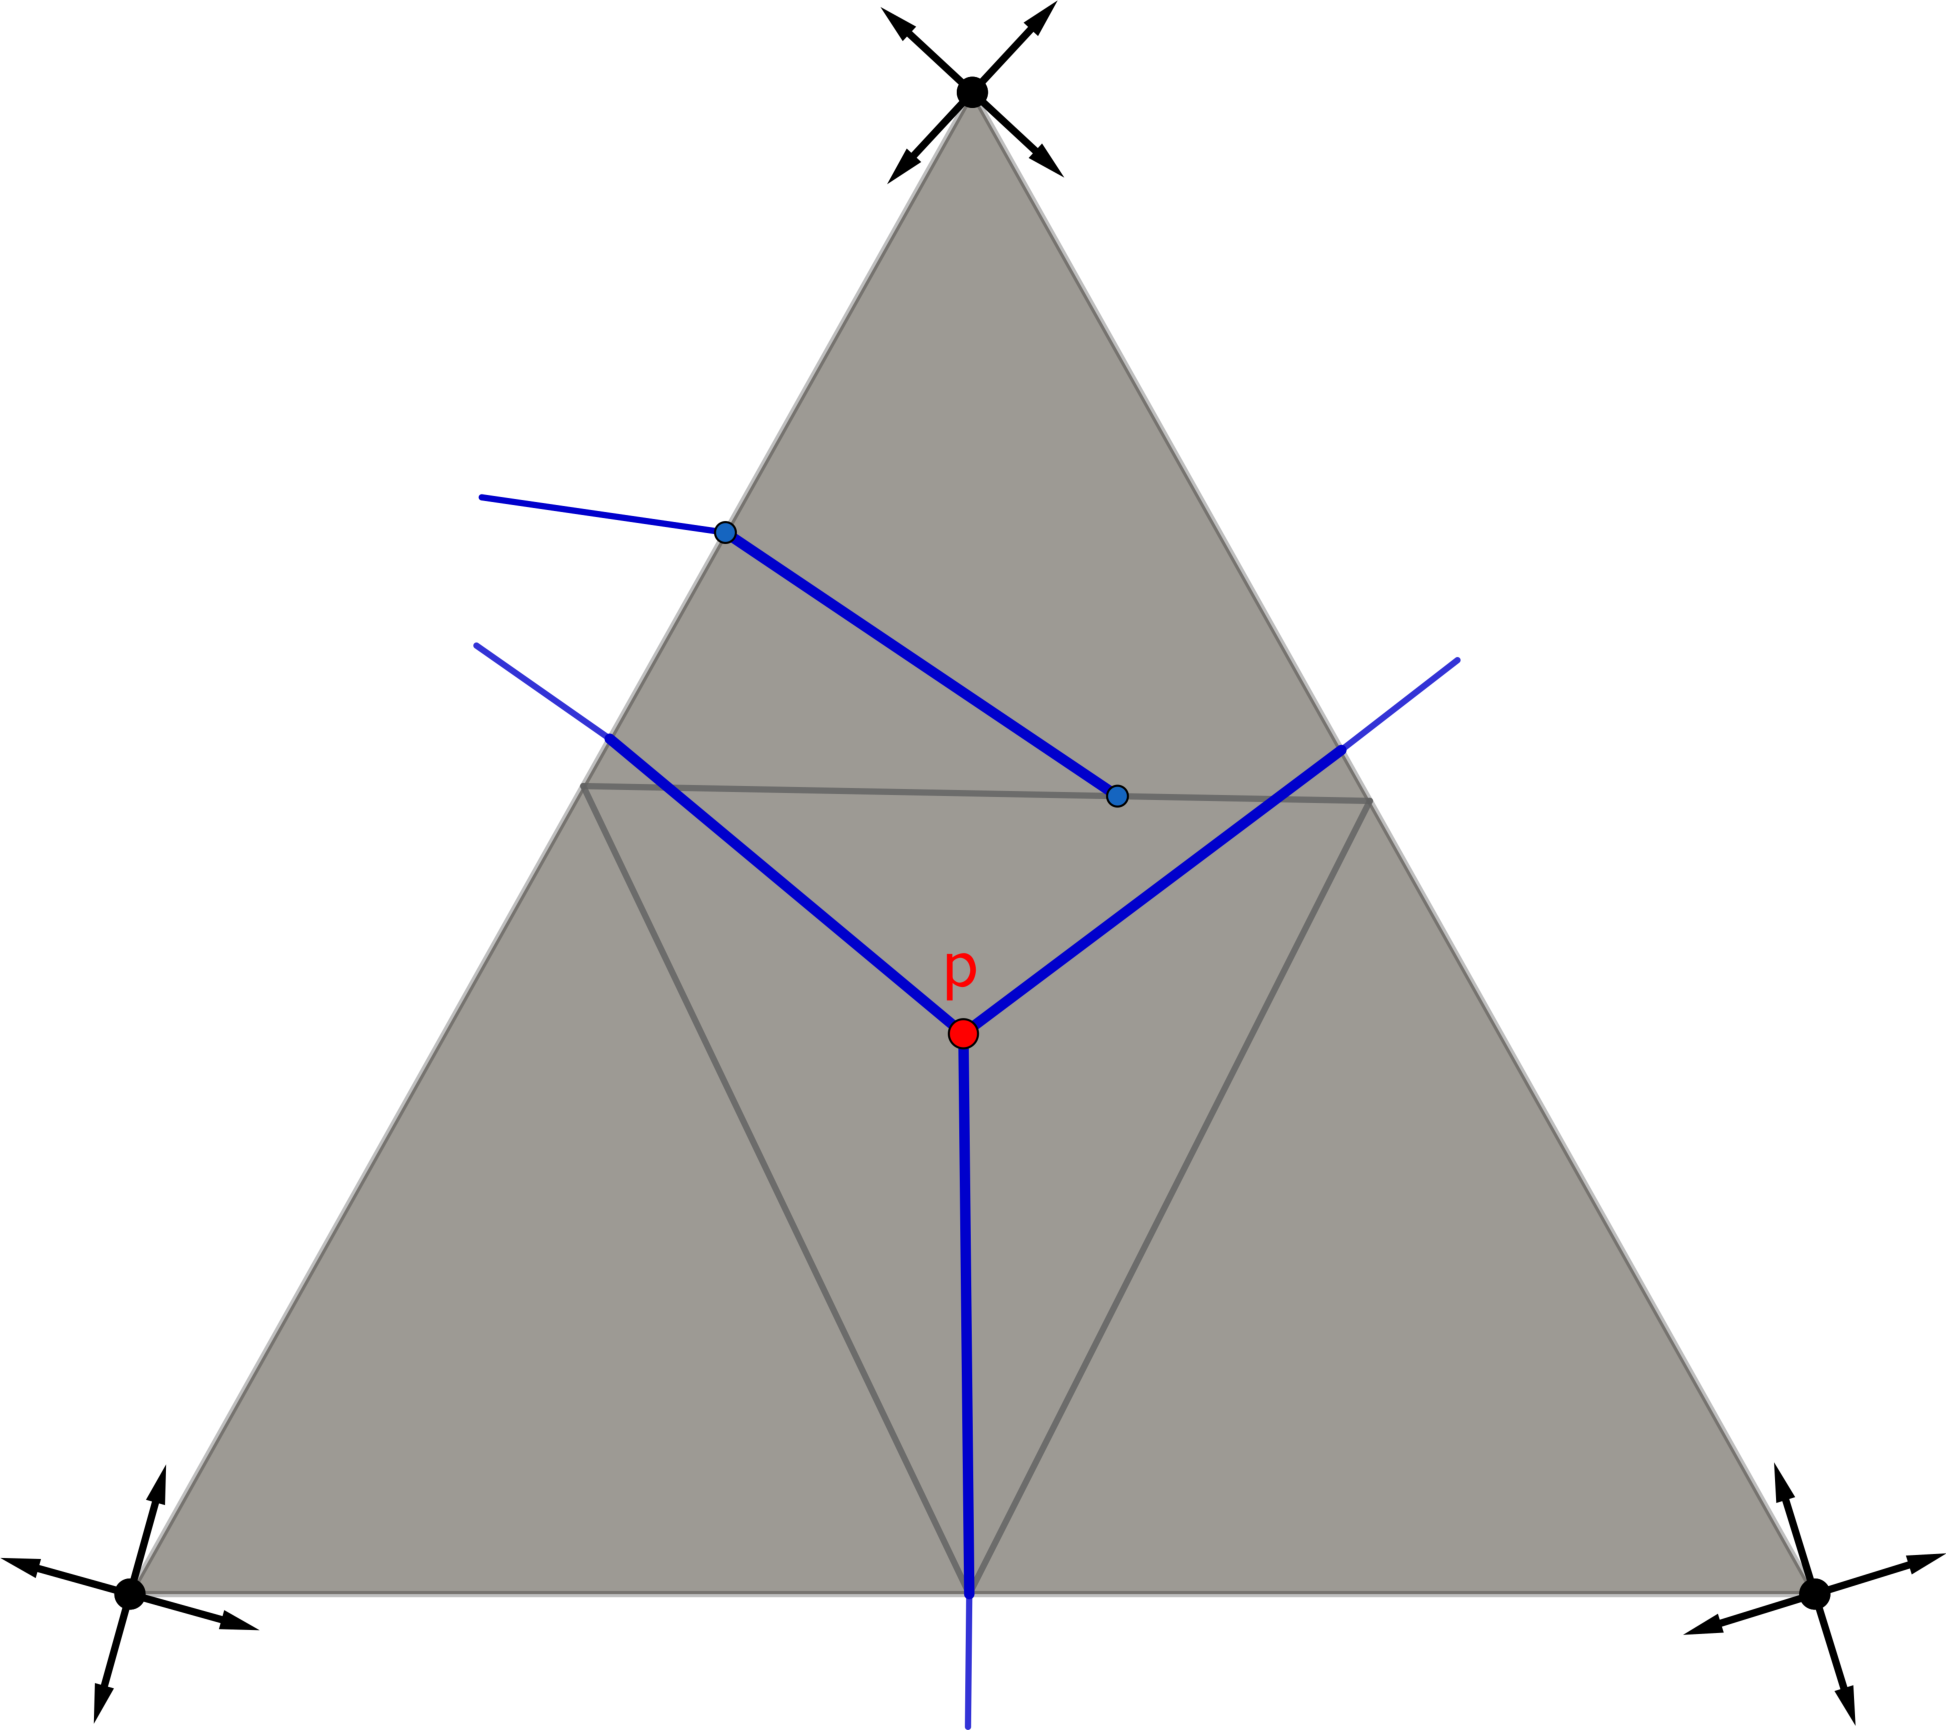
\includegraphics[scale=0.2]{images/draw_streams_sing_2.pdf}\hfill
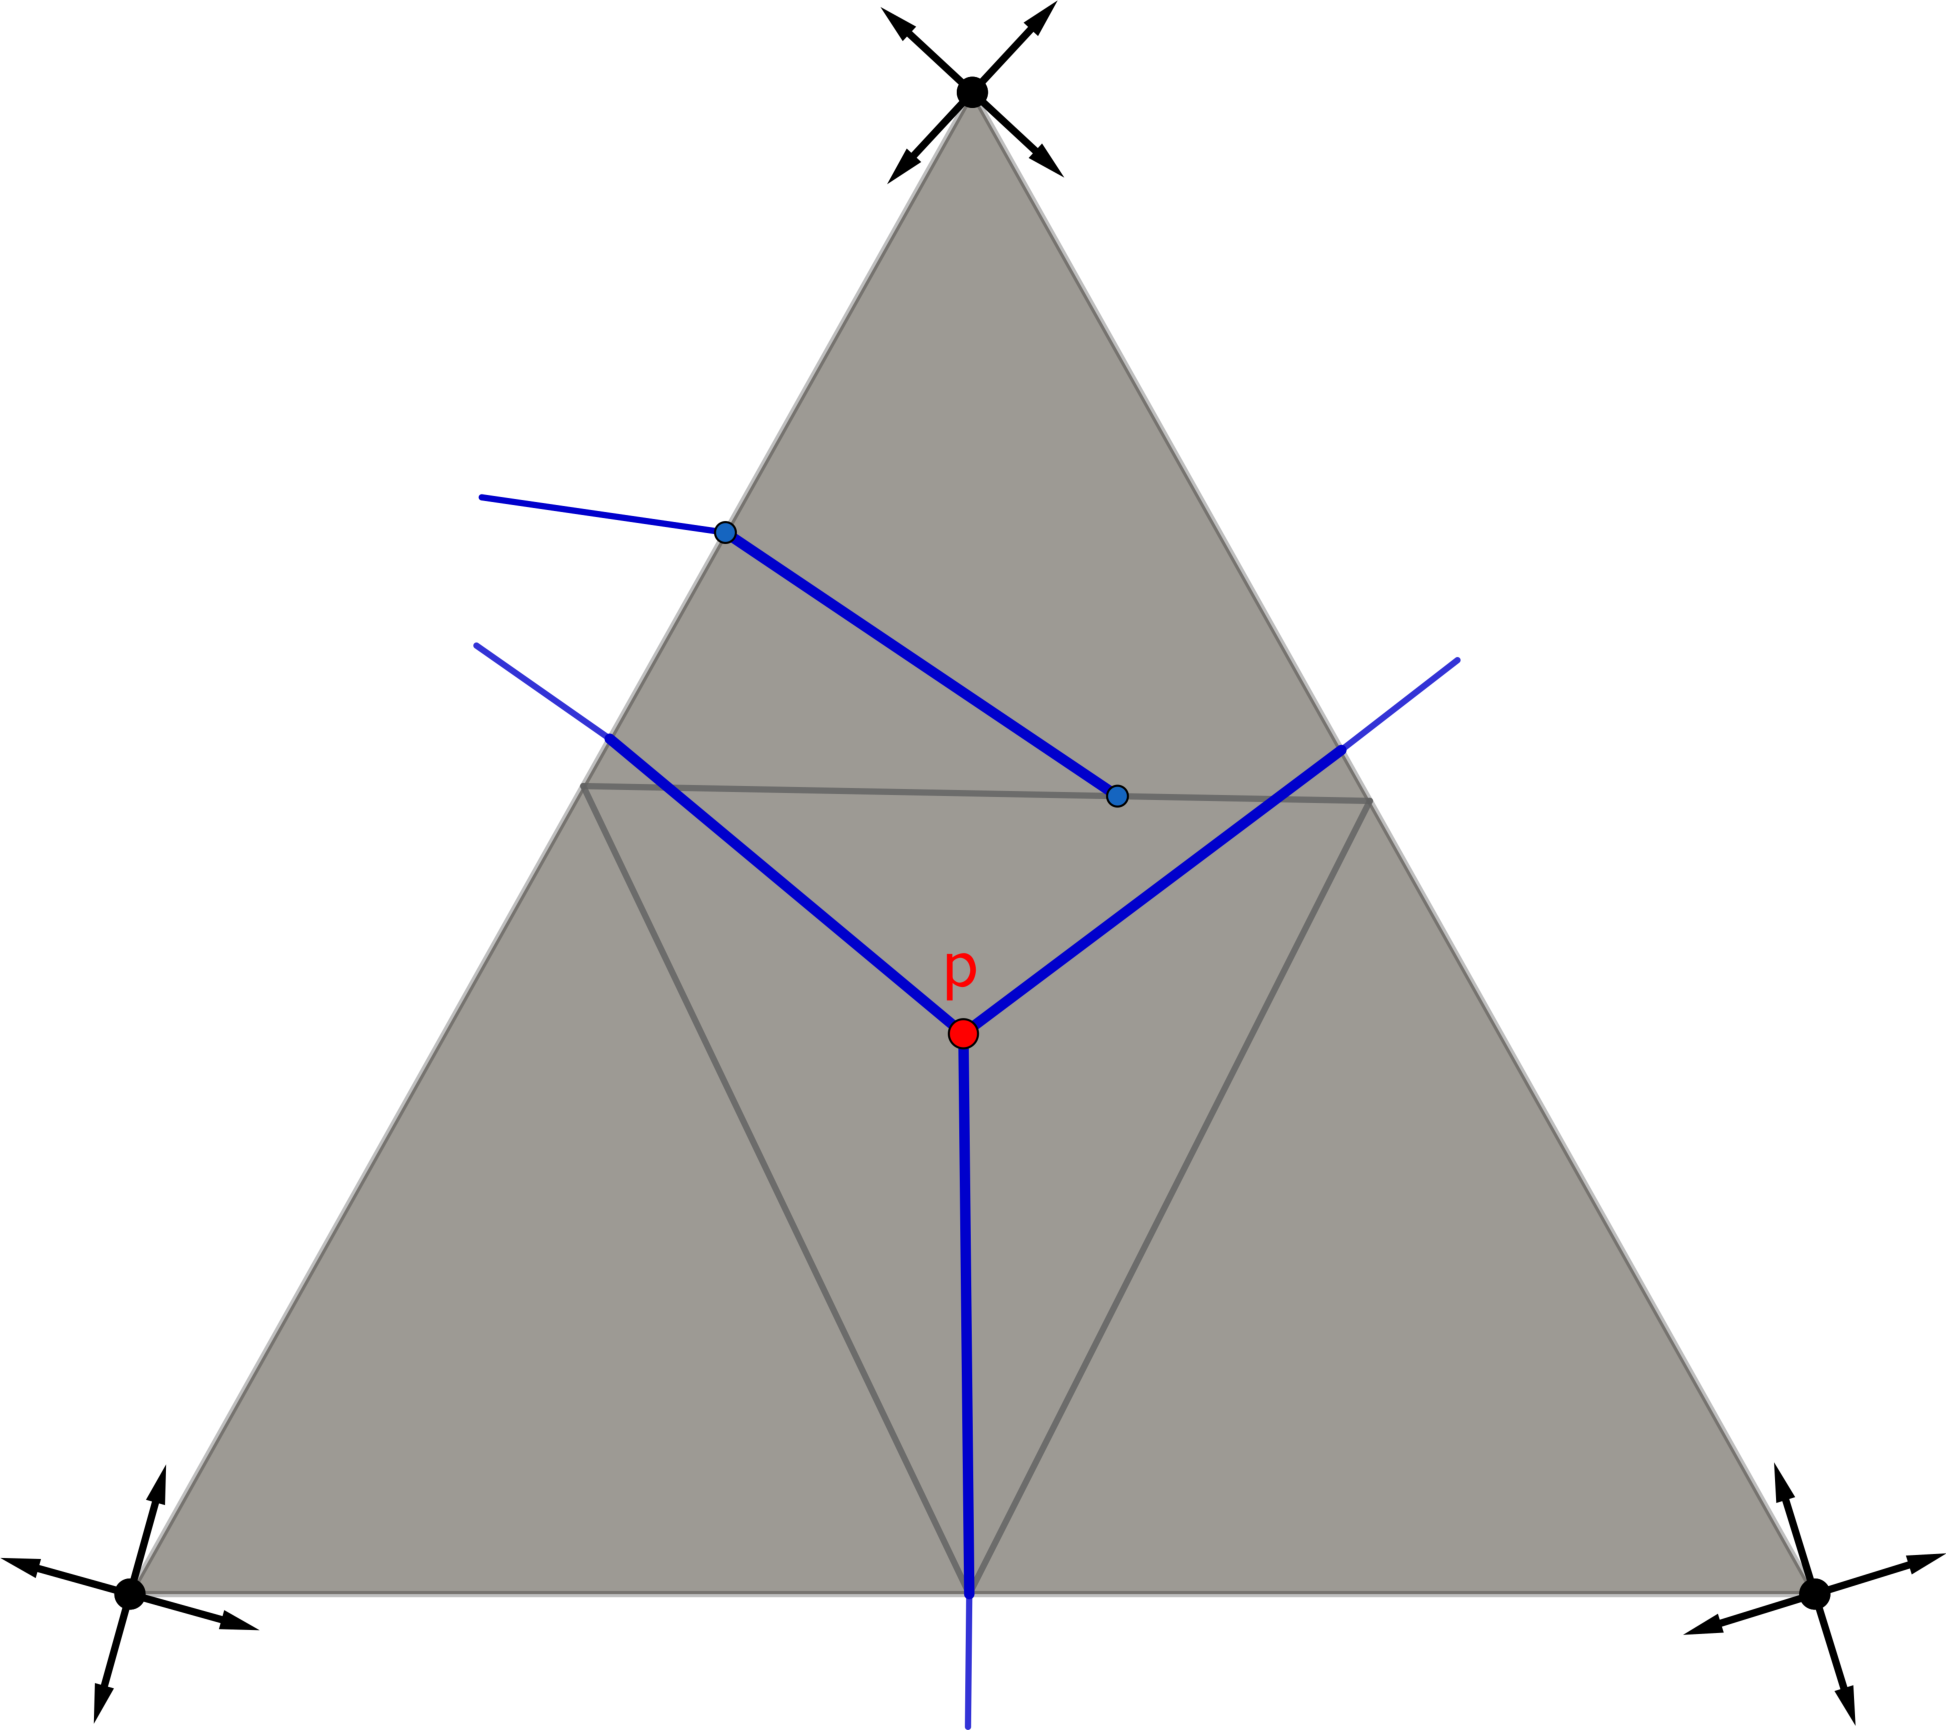
\includegraphics[scale=0.2]{images/draw_streams_sing_2.pdf}
\caption{Illustration du maillage quadrilatéral d'un anneau à partir d'un champ de croix radial.}
\label{fig:init_streams_bord}
\end{figure}

\paragraph{Fusion de séparatrices:} 
De manière similaire à ce qui est réalisé dans \cite{marcon2019high}, les séparatrices du champ de croix sont construites simultanément en incrémentant chacune d'elles progressivement, et la rencontre entre deux séparatrices est anticipée en comparant à chaque incrément, d'une part, la distance entre les derniers points calculés et, d'autre part, les directions des derniers segments construits. En d'autres termes, on cherche à déterminer si, à un moment donné, deux séparatrices données avancent dans des directions opposées et si elles sont suffisamment proches l'une de l'autre. On compare ces deux mesures à des seuils prédéfinis, et en fonction du résultat, on décide de fusionner ou non les deux séparatrices.

La fusion se réalise en créant une nouvelle séparatrice par une fusion linéaire des points des deux séparatrices impliquées. Pour se faire, chaque séparatrice est prolongée à travers $\Omega_h$ jusqu'à atteindre la position de départ de l'autre, tout en maintenant le même nombre de points pour chacune des séparatrices. L'intérêt de fusionner les séparatrices réside dans la réduction de leur nombre, ce qui se traduit directement par une diminution du nombre de régions générées lors du découpage du domaine. Nous illustrons la fusion de deux séparatrices sur la figure \ref{fig:merge_sepa}. On observe sur que la non fusion donne plus de region qui sont notemment tres etirer et non homogene par rapport aux autres ce qui induit des mesh quad non homogene.

\begin{figure}[!h]
\centering
\begin{subfigure}{0.65\textwidth}
    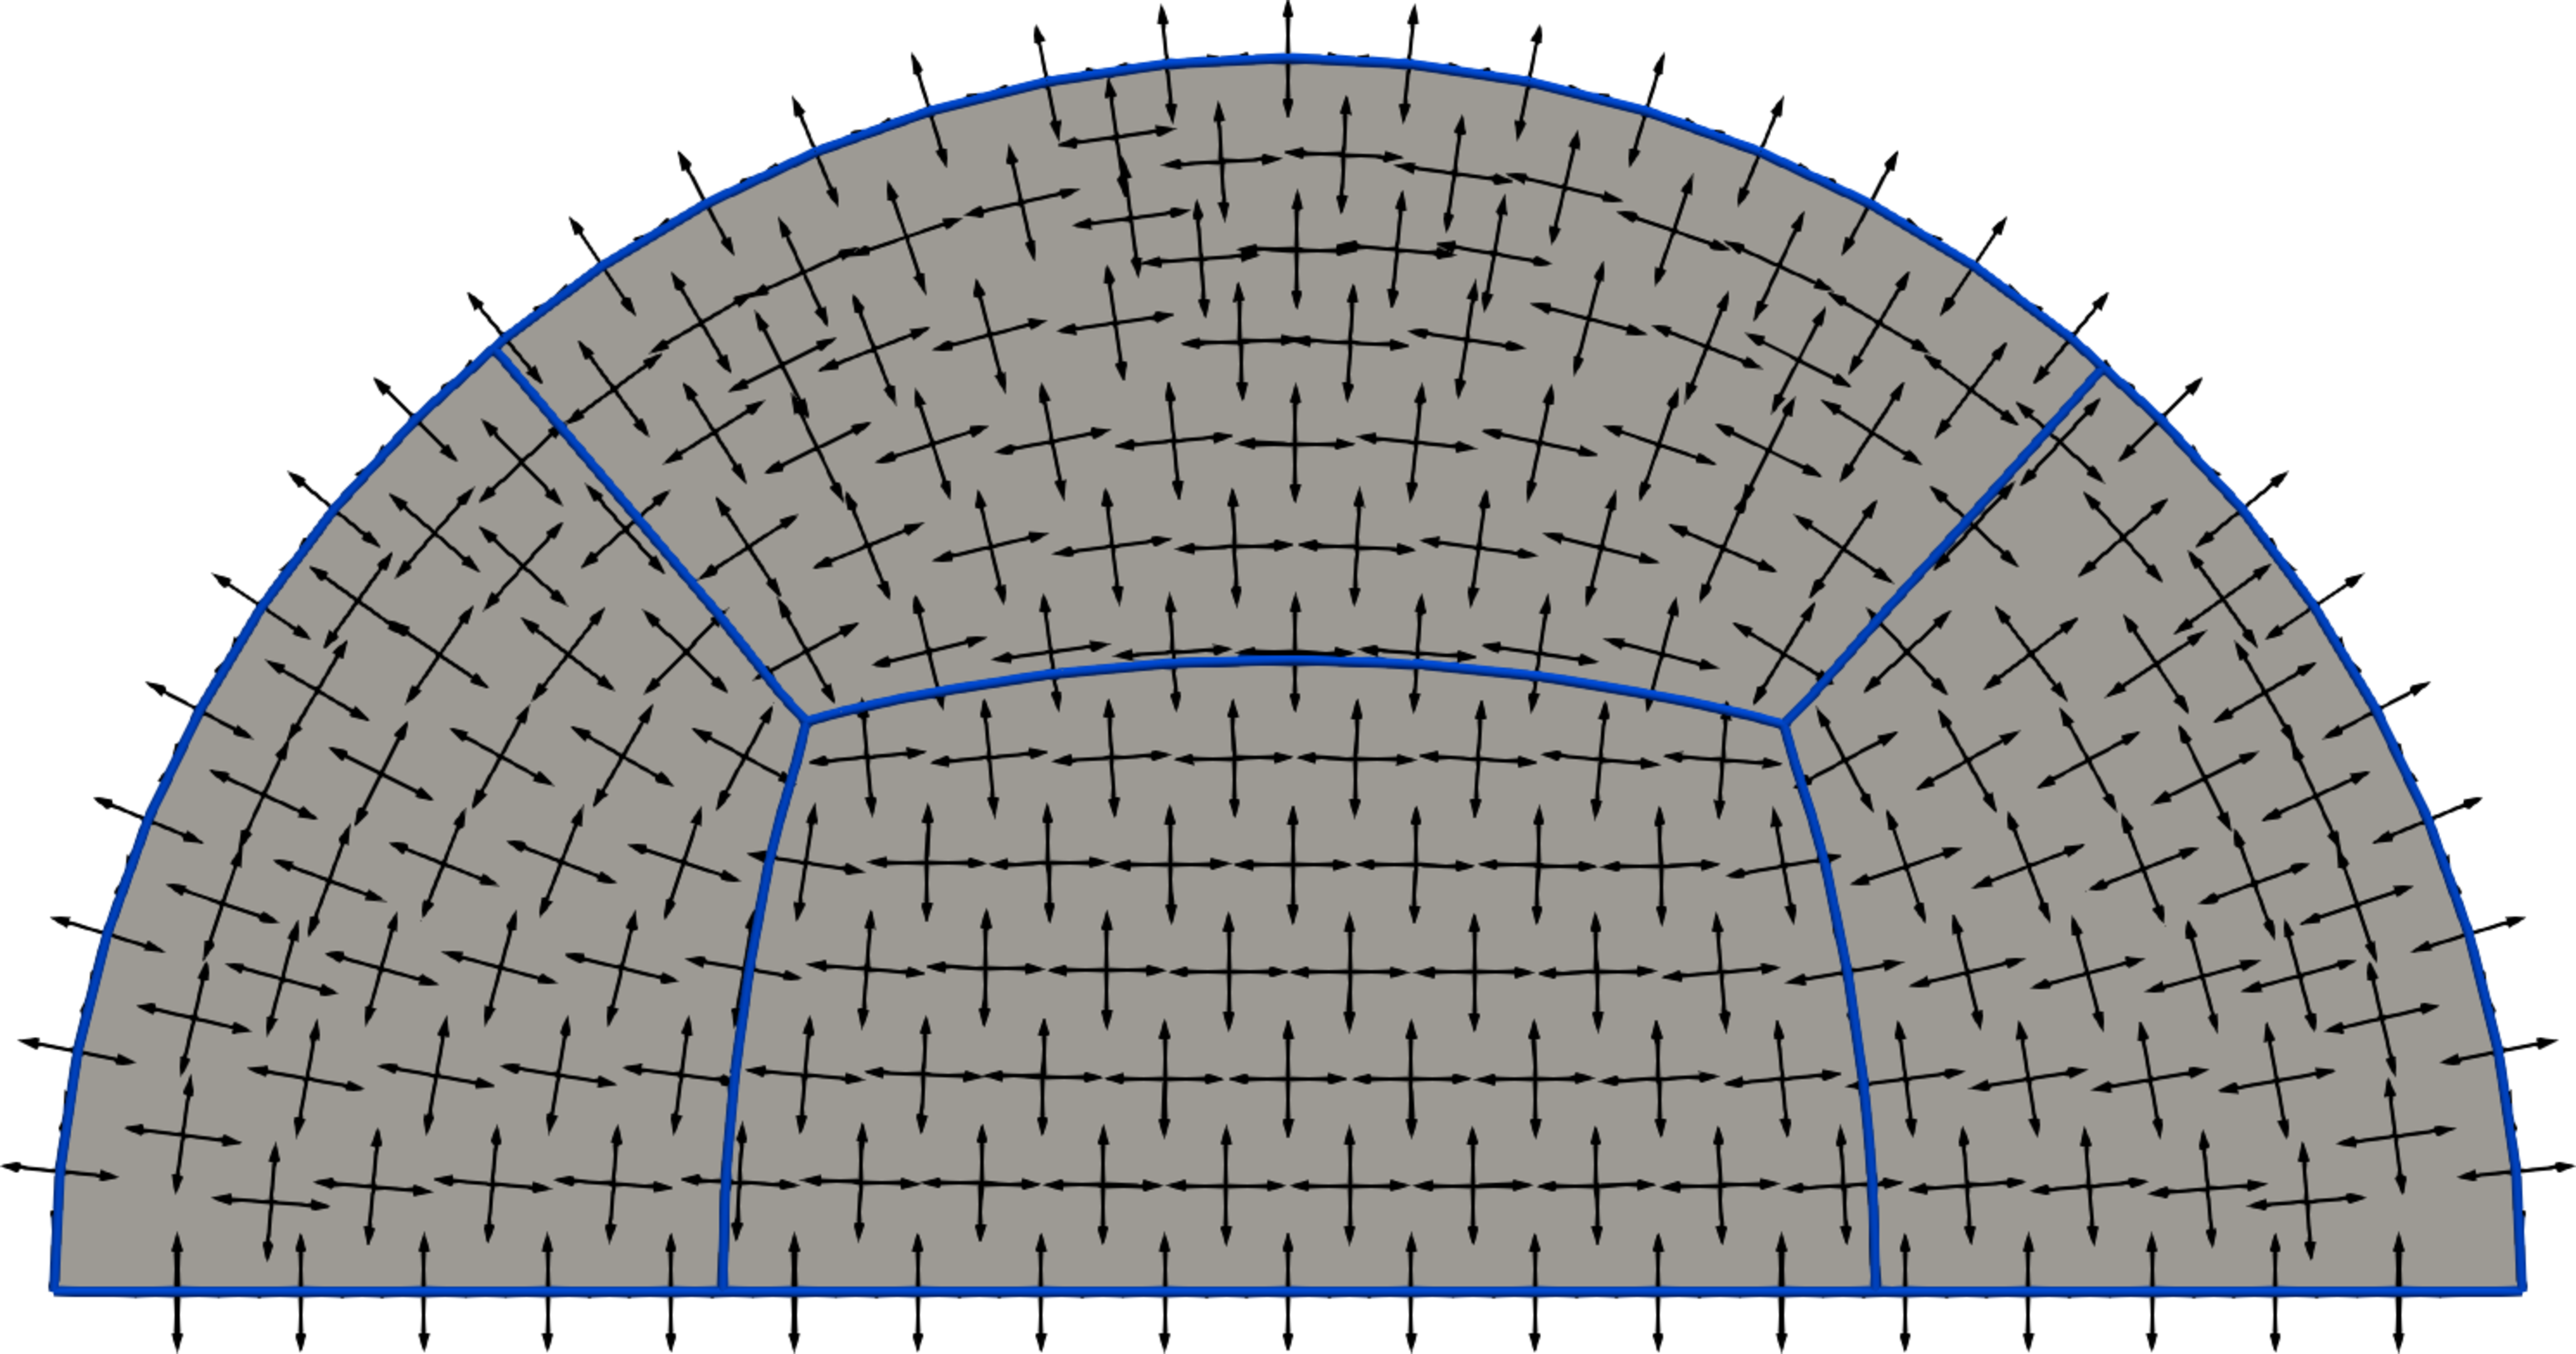
\includegraphics[width=\textwidth]{images/demi_disc_second_phi_first.pdf}
    \caption{Sans fusion}
    \label{fig:merge_sepa_first}
\end{subfigure}
\\[0.5cm]
\begin{subfigure}{0.65\textwidth}
    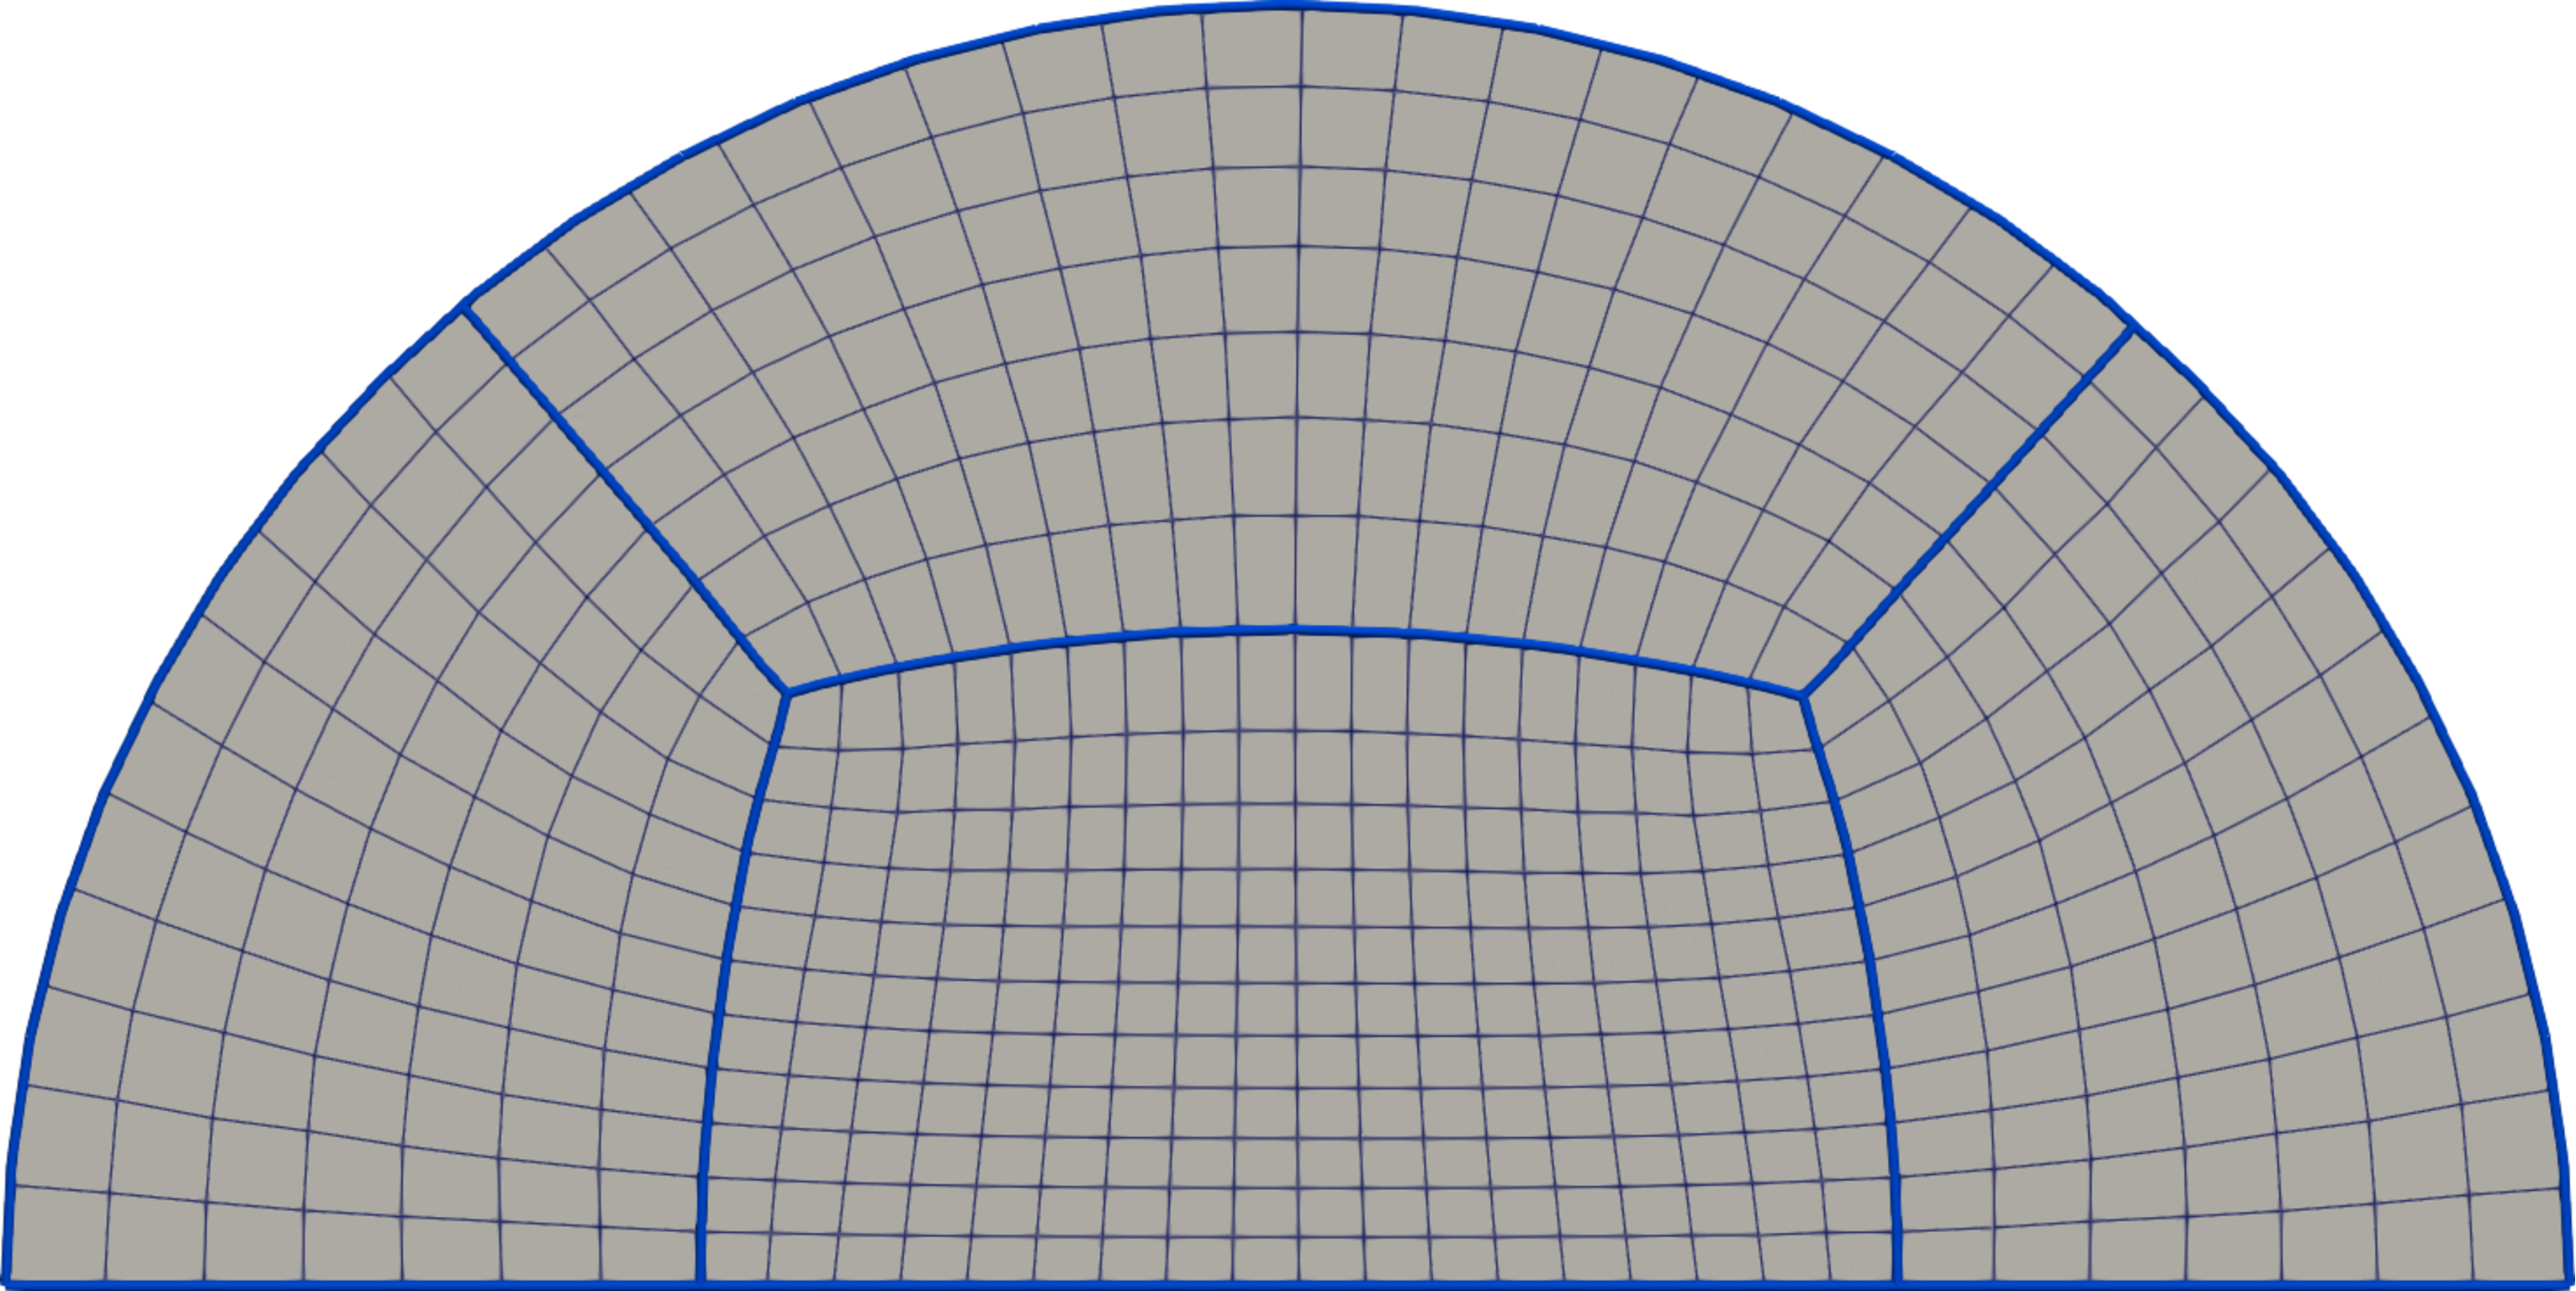
\includegraphics[width=\textwidth]{images/demi_disc_second_phi_second.pdf}
    \caption{detection fusion.}
    \label{fig:merge_sepa_second}
\end{subfigure}        
\\[0.5cm]
\begin{subfigure}{0.65\textwidth}
    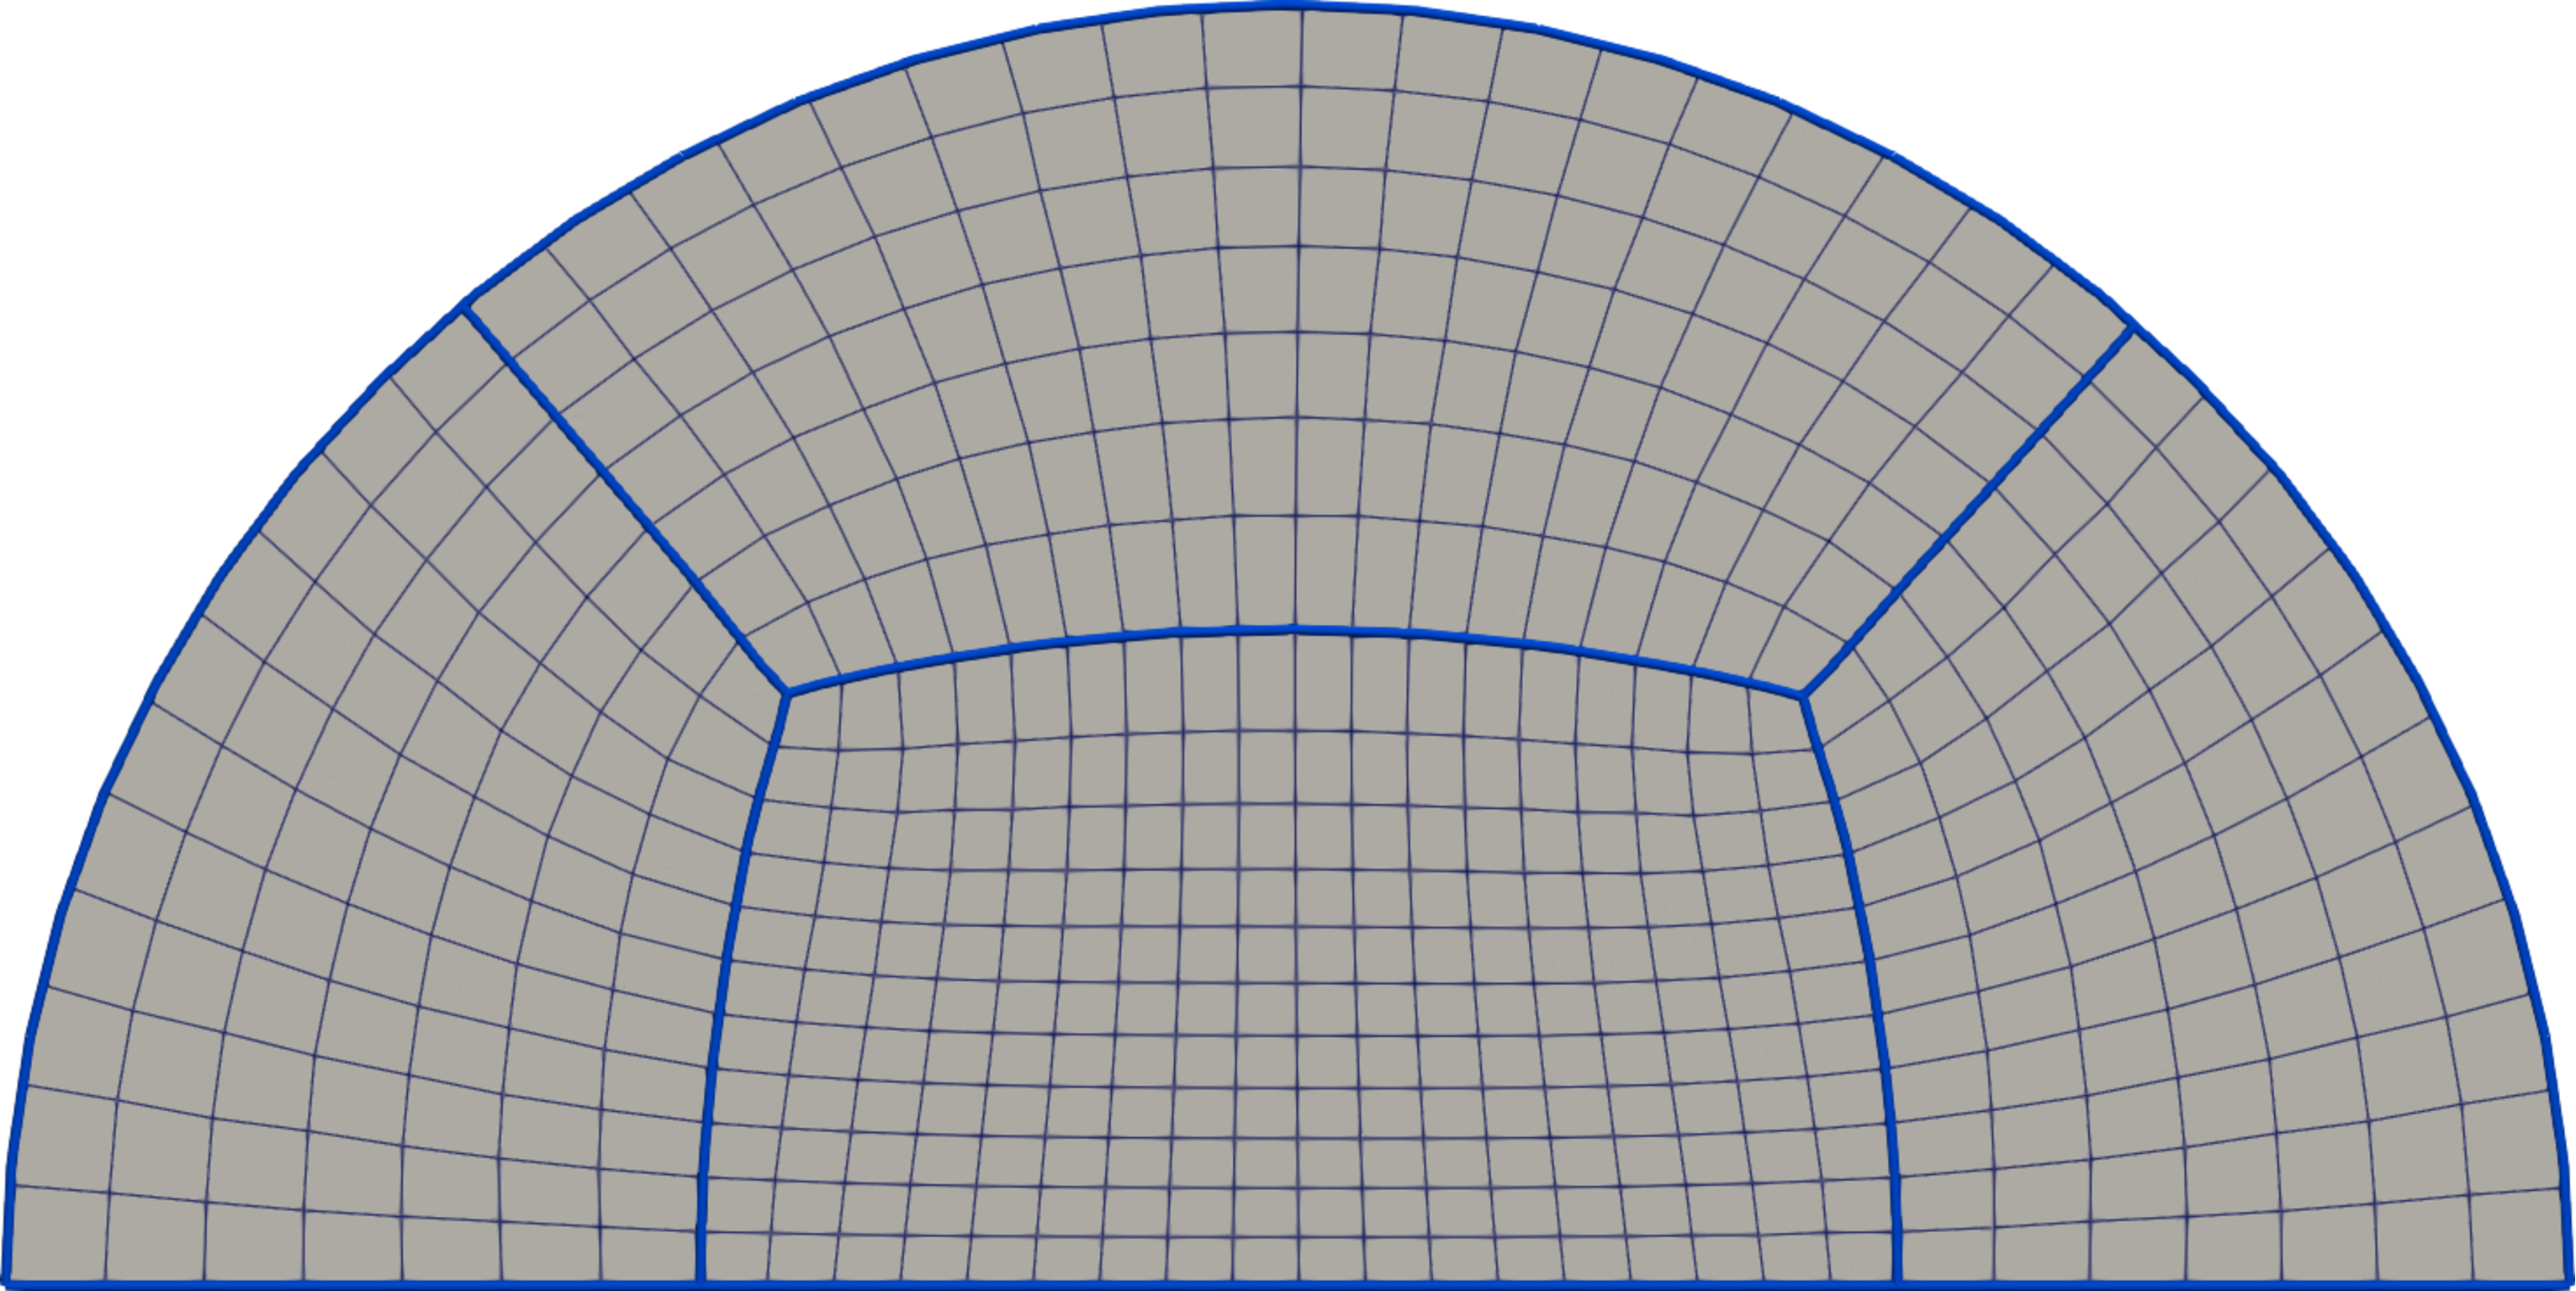
\includegraphics[width=\textwidth]{images/demi_disc_second_phi_second.pdf}
    \caption{fusion.}
    \label{fig:merge_sepa_third}
\end{subfigure}        
\caption{Illustration de l'opération d'alignement à partir du champ d'angle donné par l'équation \eqref{eqn:principe_def_phi}.}
\label{fig:merge_sepa}
\end{figure}


\subsection{Assemblage des partitions}

Une fois les séparatrices construites, le maillage triangulaire $\Omega_h$ sous-jacent à la méthode est divisé en plusieurs régions. Pour identifier ces régions, nous commençons par modifier $\Omega_h$ en un nouveau maillage. On récupère chaque région sous la forme d'un sous-maillage de $\Omega_h$ en faisant:
Localement dans chaque triangle,\\
on ajoute les points constituant les separatrices a $\Omega_h$ modifiant ainsi la topologie du maillage triangulaire initial,\\
Pour se faire, on exécute localement l'algorithme d'insertition de point localement dans chaque triangle.\\
donné par\\

\subsection{Génération du maillage quadrilatéral}

equation\\
Tracé directement dans le champ de croix\\
Interpolation transfini.

\section{Opération d'alignement}

cos laplacien rtheta...
\[\]
Nous abordons maintenant la discrétisation de l'opération d'alignement présenté dans le chapitre \ref{chap:theoritical}. Étant donné une représentation $\bar{N}_h$ du champ de croix $\bar{N}$ sur le bord $\partial\Omega_h$ de $\Omega_h$, nous cherchons à modifier $\bar{u}_h$ en construisant un nouveau champ de croix $\bar{v}_h$ qui soit aligné avec $\partial\Omega_h$. Autrement dit, on veut que pour tout $p\in\partial\Omega_h$, $\bar{v}_h(p)\in\{\bar{N}_h(p), 0\}$. Pour se faire, on commence par définir l'ensemble des points singuliers de bord du champ de croix $\bar{v}$ que l'on note $\mathcal{B}$. On associe un paramètre $I_p$ pour tout $p\in\mathcal{B}$ représentant l'indice que nous souhaitons qu'il possède dans le champ de croix $\bar{v}$ et vérifiant:
\begin{equation}
I_p=
\left\{
\begin{array}{ll}
\displaystyle\frac{k}{4}\mbox{ avec }k\in\mathbb{Z}\mbox{ et }k\leq 1&\mbox{ si }p\in\mathcal{B},\\[0.5cm]
0&\mbox{ sinon }.
\end{array}
\right.
\end{equation}
Le champ de croix $\bar{u}_h$ choisit comme champ initial doit alors vérifié $0<\#\mathcal{S}_{\bar{u}_h}<\infty$ et pour tout point $p\in\mathcal{S}_{\bar{u}_h}$, $id_{\bar{u}_h}(p)=k/4$, avec $k\in\mathbb{Z}$ et $k\leq 1$. On suppose de plus que:
\begin{equation} 
    \label{eqn:etude_hyp_u_simple}
    \theta_{\bar{u}_h}-\theta_{\bar{u}_h}=\chi(\Omega)-\sum_{p\in\mathcal{B}}I(p).
\end{equation}
Le champ de croix $\bar{v}_h$ est alors donné par:
\begin{equation}
\bar{v}_h(p)=
\left\{
\begin{array}{ll}
\mathbf{R}(\phi_h(p))\bar{u}_h(p) & \mbox{ si } p\in\Omega_h\backslash(\mathcal{B}\cup\mathcal{S}_{\bar{u}_h}),\\[0.5cm]
\bar{N}_h(p) & \mbox{ si } p\in(\mathcal{S}_{\bar{u}_h}\cap\partial\Omega_h)\backslash\mathcal{B},\\[0.5cm]
0 & \mbox{ si } p\in\mathcal{B}.
\end{array}
\right.
\label{eqn:etude_def_v_second}
\end{equation}
où $\phi_h$ est une approximation de la fonction $\phi$ définie par l'équation de Laplace suivant:\begin{equation}
\left\{
\begin{array}{lcll}
\Delta\phi &=& 0 &\mbox{ dans }\Omega_h,\\[0.5cm]
\phi_h(\gamma(t))&=&\theta^\gamma_{\bar{N}_h}(t)+\mathcal{I}(t)-\theta_{\bar{u}_h}(\gamma(t)) & \mbox{ sur } \gamma^{-1}(\partial\Omega_h\backslash(\mathcal{B}\cup\mathcal{S}_{\bar{u}_h})),
\end{array}
\right.
\end{equation}
où $\gamma$ est une paramétrisation sur $[0, 1]$ de $\partial\Omega_h$ et la fonction $\mathcal{I}$ est donnée par:
$$
\mathcal{I}(t)=\displaystyle\sum_{s\in\gamma^{-1}(\mathcal{B})}\left[\left(\pi-\widehat{\gamma(s)}-2\pi I_{\gamma(s)}\right)-\left(\displaystyle\lim\limits_{r\rightarrow s^+}\theta^{\gamma}_{\bar{N}_h}(r) - \lim\limits_{r\rightarrow s^-}\theta^{\gamma}_{\bar{N}_h}(r)\right)\right]\mathbb{1}_{[0, t]}(s),
$$
avec $\widehat{\gamma(s)}$ la mesure de l'ouverture angulaire de la frontière en $\gamma(s)$.

ne pas oublié thetah pour le non-simplement connexe


\section{Analyse de convergence}


champ de croix u isolé donc uh isolé\\

vers quoi tend Qh ?\\

On se rend compte que les normales ne match pas.\\

Je me suis aligné avec les normales d'une autre géométrie. Laquelle?\\

On a eu Qh. \\

Lorsque h tend vers 0\\

Le partitionnement Qh obtenu suite au partitionnement est 'il une decomposisition en région de quatres côtés de $\Omega_h$ ?\\

En quel sens le partitionnement Qh obtenu est;\\
On peu ainsi reconstruit le bord en ordre supérieur


\section{Génération de champs de croix}
edp\\
z-ai\\
somme flux triangle

\section*{Construction d'un maillage quadrilatéral}
De manière similaire à ce qui a été exposé dans le chapitre précédent, nous entamons d'abord la mise en place du processus de partitionnement de $\Omega_h$, puis nous revenons sur la discrétisation des différentes méthodes permettant d'aligner un champ de croix donné sur le bord du domaine sur lequel il est défini. Pour finir, nous abordons le maillage en quadrangles des régions à quatre côtés résultant du partitionnement de $\Omega_h$.


\subsection*{Traitement des bords}

\subsection*{Obtention du maillage quadrilatéral}
Description de l'interpolation transfini.

\section*{Interprétation du partitionnement}
En vrai vh pas aligné avec omegah donc pas de raison que ca marche

vh tend vers v
Sh tend vers S
Rh tend R
chap 2 marche par v S et R donc partitionnement a 4 cotés
Donc Qh est un maillage de omega



Notons que le maillage $\Omega_h$ est construit de sorte que $\mathbf{B}$ soit inclut dans l'ensemble des sommets de $\partial\Omega_h$.\\

Jusqu'à présent, nous n'avons pas supposé que nous travaillions avec une discrétisation particulière. Dans ce chapitre, nous discrétisons la méthode sur des maillages triangulaires.

Dans le chapitre précédent, les composantes de premier plan mise en jeu sont: le domaine bornée $\Omega$, l'ensemble $\mathbf{B}$ des points de $\partial\Omega$ caractérisant la géométrie de $\Omega$ et le champ de croix initial $\bar{u}$ vérifiant l'hypothèse $\mathbf{H}_1$. Avec ces données, nous construisons un champ de croix $\bar{v}$ aligné avec le bord de $\Omega$ issue des différentes opérations abordés dans le chapitre précédent. $\bar{v}$ est ensuite utilisé pour partitionner le domaine $\Omega$ en régions de quatre côtés.

Commençons par exécuter le processus d'alignement sur le champ de croix $\bar{u}_h$ puisque le champ de croix $u$ dont il est l'approximation n'a aucune raison d'être aligné par rapport à $\Omega$. Pour se faire, nous cherchons un champ d'angle noté $\phi_h$ et vérifiant l'équation suivante:

\begin{equation}
\left\{
\begin{array}{lcl}
\Delta\phi_h &=& 0 \mbox{ dans }\Omega_h,\\[0.25cm]
\phi_h &=& \theta_{\Bar{N}_h}-\theta_{\bar{u}_h} \mbox{ sur } \partial\Omega_h.
\end{array}
\right.
\label{eq:phi_computation_omega_h}
\end{equation}

où $\bar{N}_h$ correspond au champ de croix de la normale extérieur de $\partial\Omega_h$. Remarquons que $\bar{N}_h$ est défini sur les arêtes de $\partial\Omega_h$ mais n'est pas défini sur les sommets de $\partial\Omega_h$. Autrement dit, le champ de croix $\bar{N}_h$ n'est pas compatible avec l'ensemble $\mathbf{B}$ puisque les points singuliers de $\bar{N}_h$ ne coïncident pas avec les points de l'ensemble $\mathbf{B}$. 

%Cela implique que suite au processus d'alignement, le champ de croix résultant $v_h=R(\phi_h)u_h$ aura comme point singulier de bord tous les sommets de $\partial\Omega_h$ autrement dit, les points singuliers de $\bar{v}_h$ ne coincideront pas avec les points de l'ensemble $\mathbf{B}$. Ainsi, un découpage  Le champ de croix $\bar{v}_h$ ainsi construit ne peut donc être une approximation du champ de croix $v$ dont les points singuliers correspondent à l'ensemble $\mathbf{B}$ (voir chapitre \ref{chap:theoritical}).

Pour palier à ce problème, nous modifions la définition du champ de croix normal. Supposons que l'on puisse définir un champ de croix $\widetilde{N}_h$ sur $\partial\Omega_h$ tel que les points singuliers de $\widetilde{N}_h$ correspondent exactement aux points de l'ensemble $\mathbf{B}$. L'équation \eqref{eq:phi_computation_omega_h} devient alors:

\begin{equation}
\left\{
\begin{array}{lcl}
\Delta\phi_h &=& 0 \mbox{ dans }\Omega_h,\\[0.25cm]
\phi_h &=& \theta_{\widetilde{N}_h}-\theta_{\bar{u}_h} \mbox{ sur } \partial\Omega_h.
\end{array}
\right.
\label{eq:phi_computation_omega_tilde}
\end{equation}

La résolution de l'équation \eqref{eq:phi_computation_omega_tilde} permet de construire le champ de croix $\bar{v}_h$ sur $\Omega_h$ définit par:
$$\bar{v}_h:p\in\Omega_h\longrightarrow \bar{v}_h(p)=\mathbf{R}(\phi_h(p))\bar{u}_h(p).$$

\newpage

On ne peut interpoler directement le champ de croix, on passe par un champ de vecteur intermédiare appelé champ de représentation \ref{},\\
\[\]
Cependant, il est clair que $\bar{v}_h$ n'est pas aligné avec $\partial\Omega_h$ puisque $\bar{v}_h=\widetilde{N}_h$ sur $\partial\Omega_h$. Autrement dit, le champ de croix $\bar{v}_h$ est aligné avec un domaine que nous notons $\widetilde{\Omega}_h$ et dont la normale extérieure est associé au champ de croix $\widetilde{N}_h$. $\bar{v}_h$ n'étant pas défini sur $\widetilde{\Omega}_h$ nous définissons une opération appelé \emph{lift} et noté $\mathbf{L}$ permettant de transporté une fonction définit sur un domaine vers un autre domaine. Nous désignons alors par $\widetilde{v}_h=\mathbf{L}_{\Omega_h}^{\widetilde{\Omega}_h}\bar{v}_h$ le lift de $\bar{v}_h$ de $\Omega_h$ vers $\widetilde{\Omega}_h$. Le champ de croix $\widetilde{v}_h$ ainsi défini est aligné avec $\partial\widetilde{\Omega}_h$ (bord de $\widetilde{\Omega}_h$) ce qui nous permet d'appliquer l'algorithme de partitionnement définit dans le chapitre \ref{chap:theoritical} à $\widetilde{v}_h$ sur $\widetilde{\Omega}_h$.

\subsection*{Définition de $\widetilde{N}_h$ et $\widetilde{\Omega}_h$}

\subsection*{Définition du Lift}

\subsection*{Discussion sur $Q_h$}

utiliser dans l'équation \eqref{eq:phi_computation_omega_h} en définissant le champ de croix $\widetilde{N}$ de la manière suivante:

$$
\forall p\in\partial\Omega_h,~~\widetilde{N}(p)=
\left\{
\begin{array}{lcl}
,\\[0.25cm]
.
\end{array}
\right.
$$

L'équation \eqref{eq:phi_computation_omega_h} devient alors:


Suite à la résolution de l'équation \eqref{eq:phi_computation_omega_tilde} sur $\Omega_h$, on peut construire le champ de croix $\bar{v}_h=\mathbf{R}(\phi_h)\bar{u}_h$ sur $\Omega_h$. On remarque alors que le champ de croix $\bar{v}_h$ ainsi construit n'est pas aligné avec $\Omega_h$.

\[\]
Définition de $\widetilde{\Omega}$

\begin{figure}[!h]
\centering
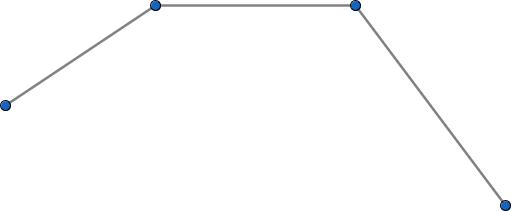
\includegraphics[scale=0.65]{images/Omega_h_tilde.png}
\caption{}
\label{fig:omega_h_tilde}
\end{figure}

\[\]
Définition du lift $\mathbf{L}$

\[\]
Définition de $\widetilde{v}=\mathbf{L}_{\Omega_h}^{\widetilde{\Omega}}v_h$

\[\]
Comparaison de $v$ et $\widetilde{v}$

\begin{eqnarray*}
\|v-\mathbf{L}_{\widetilde{\Omega}}^\Omega\widetilde{v}\|&\leq&\|\mathbf{R}(\phi)u-\mathbf{R}(\phi)\mathbf{L}_{\Omega_h}^\Omega u_h\|+\|\mathbf{R}(\phi)\mathbf{L}_{\Omega_h}^\Omega u_h - \mathbf{L}_{\widetilde{\Omega}}^\Omega\widetilde{v}\|\\
&\leq&\|\mathbf{R}(\phi)u-\mathbf{R}(\phi)\mathbf{L}_{\Omega_h}^\Omega u_h\|+\|\mathbf{R}(\phi)\mathbf{L}_{\Omega_h}^\Omega u_h - \mathbf{R}(\mathbf{L}_{\Omega_h}^\Omega\phi_h)\mathbf{L}_{\Omega_h}^\Omega u_h\|+\\
&&\| \mathbf{R}(\mathbf{L}_{\Omega_h}^\Omega\phi_h)\mathbf{L}_{\Omega_h}^\Omega u_h - \mathbf{L}_{\widetilde{\Omega}}^\Omega\mathbf{L}_{\Omega_h}^{\widetilde{\Omega}}v_h\|\\
&\leq&\|\mathbf{R}(\phi)u-\mathbf{R}(\phi)\mathbf{L}_{\Omega_h}^\Omega u_h\|+\|\mathbf{R}(\phi)\mathbf{L}_{\Omega_h}^\Omega u_h - \mathbf{R}(\mathbf{L}_{\Omega_h}^\Omega\phi_h)\mathbf{L}_{\Omega_h}^\Omega u_h\|+\\
&&\| \mathbf{R}(\mathbf{L}_{\Omega_h}^\Omega\phi_h)\mathbf{L}_{\Omega_h}^\Omega u_h - \mathbf{L}_{\widetilde{\Omega}}^\Omega\mathbf{L}_{\Omega_h}^{\widetilde{\Omega}}\mathbf{R}(\phi_h)u_h\|
\end{eqnarray*}



%\begin{figure}[!h]
%    \centering
%    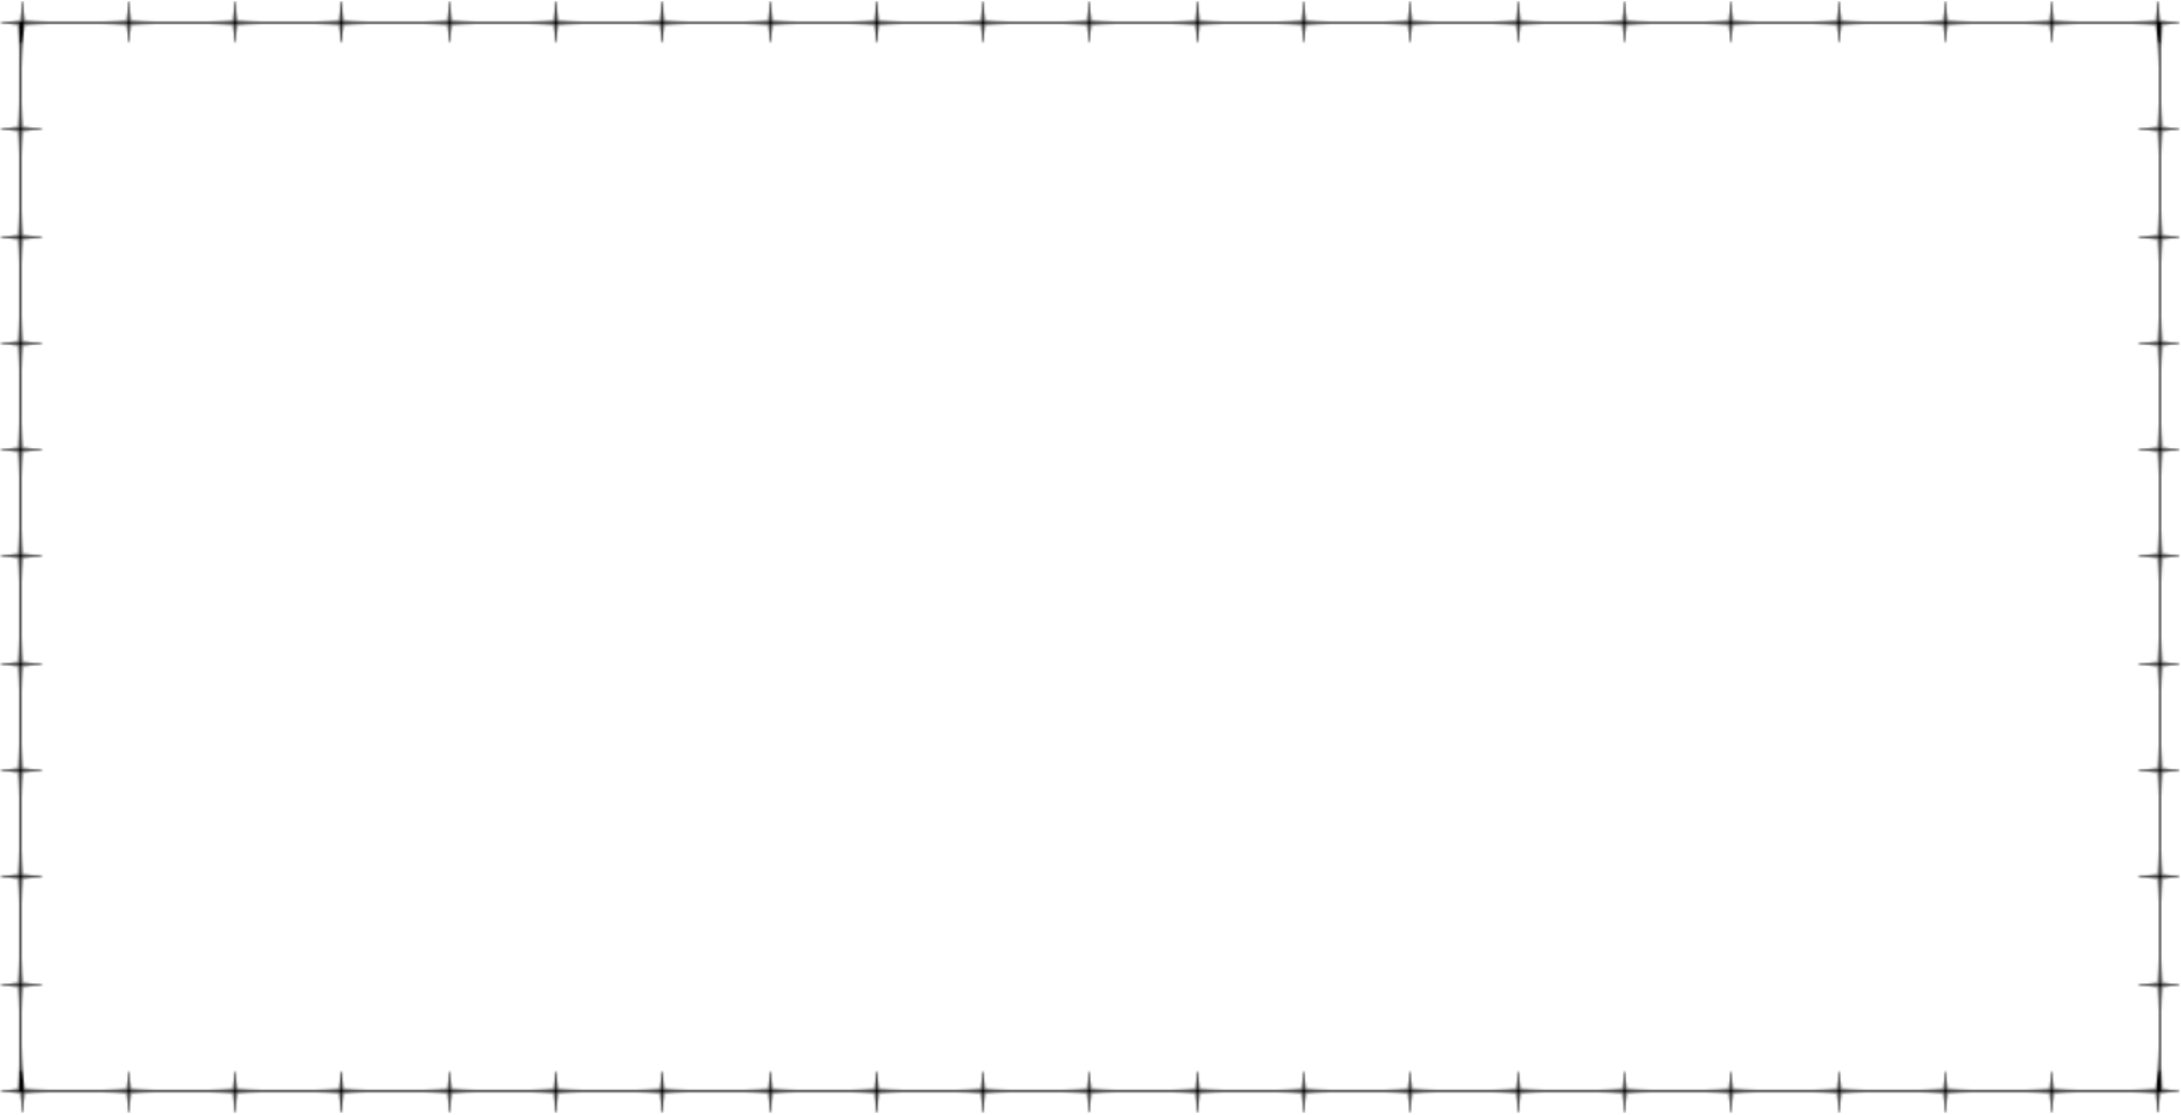
\includegraphics[scale=0.3]{images/im_default.pdf}
%    \caption{Maillage triangulaire d'un domaine quelconque}
%    \label{fig:mesh_tri_dom_quelc}
%\end{figure}
%Nous utilisons des tuples d'indices de sommets pour spécifier les simplices - par exemple, ijk est un triangle avec les sommets i, j, k ∈ V. Les indices apparaissant des deux côtés d'une équation sont fixés dans les sommes, par exemple ai j = Pi jk ∈ F bi jk signifie une somme uniquement sur les triangles ijk ∈ F contenant l'arête ij.

\section*{Algorithmes}
\color{blue}
remarque sur le tracé des "sreamlines" dans un triangle singulier en comparaison avec ce que fait viertel sachant que le champ n'est pas linéaire dans un tel triangle
\color{black}


\section*{Exemples}

\begin{figure}[!h]
\centering
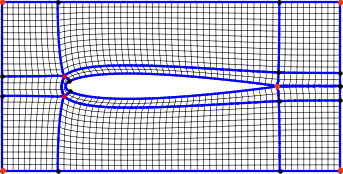
\includegraphics[scale=0.65]{images/nacas_normal.png}\hspace{0.5cm}
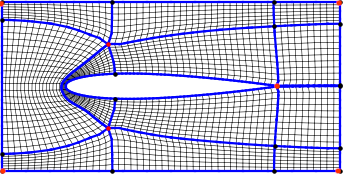
\includegraphics[scale=0.65]{images/naca_obus.png}
\caption{Mesh of Naca0012 with two different configurations of singular points. The initial cross-fields were obtained using formula (\ref{eq:z-ai}) .}
\label{connexe2}
\end{figure}

Structure de donnée\\
représentation des multimatériau\\


structure de donnée mesh
\[\]
generation champ de croix\\
discretisation par vertex\\
alignement champ de croix
\[\]
index\\
seul type 1 0 -1
\begin{figure}
    \centering
    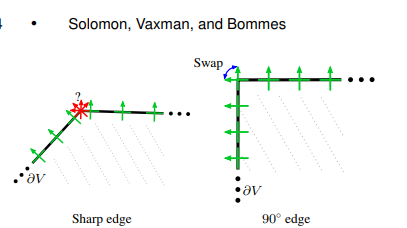
\includegraphics{images/inspi_1.png}
    \caption{Caption}
    \label{fig:enter-label}
\end{figure}

N'importe quel champ $\longrightarrow$  mesh quad\\*
preserver les points singuliers\\
Montrer simplement phi=N-U et sa trace\\
deplacer ensuite les singularité vers où ion veut

;\begin{comment}
Complementary Operations
Irregular Vertex Cancellation: We can move a v3 vertex to col-
lide with a v5 vertex, or vice versa, by applying multiple pair-wise
movement operations. When one v3 and one v5 vertex collide they
cancel each other and both become regular. At least one other ir-
regular vertex needs to be involved in this cancellation. In this fash-
ion we develop a 3 − 5 pair cancellation operation. It is possible
that the last step of a 3 − 5 pair cancellation is equivalent to one
3 − 3 − 5 − 5 removal operation and two pairs of irregular vertices
are canceled at once. Examples can be found in Figures 16 and 17.
Irregular Vertex Merging: A 3 − 3 pair can be merged to a v2
vertex and a 5 − 5 pair can be merged to a v6 vertex when their
graph distance is even. Theorems 7.2 and 7.3 provide the theoretical
analysis that is related to such a merge.
Irregular Vertex Alignment: Under the assumptions of Theo-
rems 7.2 and 7.3, arbitrary 3 − 3 and 5 − 5 pairs can be aligned
by applying multiple movement operations until d1 = 0 or d2 = 0.
Smoothing: We use iterative Laplacian mesh smoothing to im-
prove the geometry if the connectivity edits degrade the shape of
the mesh above a user-defined tolerance. The user can select uni-
form weights or cord-length weights, and elect to preserve sharp
features by constraining the positions of vertices on sharp edges.
The smoothing scheme can improve the aspect ratios of modified
faces. After each iteration all vertices are projected back onto the
original mesh. We have also experimented with a scheme in which
newly generated vertices are pulled towards vertices in the origi-
nal mesh if the distance between the new and original vertices is
above a threshold. The projection and pulling scheme can narrow
the difference to the original mesh. 
9 Connectivity Editing for Quadrilateral Meshes
Chi-Han Peng∗
Arizona State University
Eugene Zhang†
Oregon State University
Yoshihiro Kobayashi‡
Arizona State University
Peter Wonka§
Arizona State University /
KAUST
\end{comment}
